%% LaTeX2e class for student theses
%% sections/evaluation.tex
%% 
%% Karlsruhe Institute of Technology
%% Institute for Program Structures and Data Organization
%% Chair for Software Design and Quality (SDQ)
%%
%% Dr.-Ing. Erik Burger
%% burger@kit.edu
%%
%% Version 1.3.6, 2022-09-28

\chapter{Evaluation}
\label{ch:Evaluation}

In this section we will present the results of our experiments. Our experiments are split into two parts. The first part is the evaluation of our novel
Continual Active Learning Approach and the second part is evaluating the performance our the Continual Active Learning approach when applied to Model Stealing.
In each of these respective subsections we will first describe the experiments schedule for each part and then present the results of the experiments.



\section{Continual Active Learning}
\label{sec:CAL}
In this section we will evaluate the results of our experiments using continual active learning in its classic setting. First, we experiment with regularization-based
continual learning strategies. Next, we evaluate the performance of our custom replay strategy from section \ref{sec:Methodology:ReplayStrategy}. Finally, we
test the combination of exemplar rehearsal continual learning and representation-based active learning.

\subsection{Regularization-based Continual Learning}
\label{sec:Evaluation:Results:CAL:ALRegCL}
We start our experiments by running each combination of the Active Learning strategies \gls{bald},\gls{badge},CoreSet,\gls{lc} and Random with the Continual Learning
strategies Naive, \gls{ewc}, \gls{mas}, \gls{alasso} and \gls{imm}. We use the dataset CIFAR-10, the Neural Network Architecture ResNet18 and a batch size of 4000 for these experiments. For each experiment,
we present the validation accuracy with increasing size of the labeled pool as well as the overall execution time of each experiment. The results by validation accuracy and by execution time are shown in 
Figure \cite{fig:Evaluation:CAL:4000bAcc} and Table \ref{fig:Evaluation:CAL:4000bTime}, respectively.\par

First, we evaluate the results for random sampling. In terms of execution time, there is a large gap between the baseline and the continual learning strategies. \gls{imm} is
the fastest method, followed by \gls{mas}, \gls{ewc} and Naive who perform on the same level. \gls{alasso} is the slowest continual learning strategy, but is still about six times as fast as the baseline. 
In terms of validation accuracy, the baseline outperforms all continual learning strategies by at least ten percentage points. Naive, \gls{ewc} and \gls{imm} demonstrate a similar accuracy
progression, with \gls{ewc} and Naive marginally outperforming \gls{imm}. \gls{mas} has a higher validation accuracy than the three aforementioned strategies in the beginning, but fails to keep up with their
continuous increase in validation accuracy. \gls{alasso} starts of with a higher validation accuracy than the other continual learning strategies, but falls behind at around 8,000 samples due to exploding
gradients. \par
 

Next, we re-run the previous experiment using \gls{lc}. In terms of execution time, the results are similar to the experiment with random sampling. \gls{alasso} is again the slowest strategy,
followed by \gls{mas}, \gls{ewc}, \gls{imm} and Naive. All continual learning strategies are significantly faster than the baseline, with \gls{alasso} being about six times as fast and Naive
about ten times as fast. The gap in validation accuracy between the baseline and the continual learning strategies remains significant and increases during the last 25,000 samples. 
\gls{imm}, \gls{ewc} and Naive perform almost identically across the experiment with \gls{mas} following closely and outperforming the remaining strategies within the last 5000 samples. The four aforementioned methods
experience a decrease in validation accuracy caused by the inferior representativeness of the final batches. \gls{alasso} starts competitively, but suffers from a heavy decrease in validation accuracy at around 8000 samples,
which is again caused by exploding gradients. \par


The third experiment is run with the active learning strategy \gls{bald}. The ranking of execution time of the continual
learning strategies and the baseline is similar to the previous experiments with Random and \gls{lc}. In terms of accuracy, the baseline outperforms the continual learning strategies significantly. The gap between
in validation accuracy is most prominent at roughly 15,000 samples and in the final batch. Naive, \gls{imm} and \gls{ewc} perform similar, showing an
s-shaped validation accuracy curve. The performance of \gls{mas} follows a similar curve, however \gls{mas} performs better in the first half of the experiment, and worse in the second half compared to the
three former strategies. Since we use ResNet18, which does not contain dropout layers, we are unable to run Monte Carlo dropout to accurately estimate $\mathbb{E}_{\theta \sim p(\theta \mid L)} [H[y \mid x, \theta]]$.
This leads to the inferior performance of \gls{bald} compared to the other active learning strategies. \gls{alasso} starts off as
the best continual learning strategy, but its validation accuracy decreases steadily over the course of the experiment, which is again caused by exploding gradients. \par 



We now run the experiment with the identical setup using CoreSet. The gap in execution time between the baseline and the continual learning 
strategies remains significant. \gls{imm} is the fastest continual learning strategy, being about 6 times as fast as the baseline. On the other hand, \gls{alasso} is the slowest Continual Learning strategy,
boasting around one fourth of the execution time of the baseline. In terms of validation accuracy, the accuracy progression strongly resembles the experiment with \gls{lc}. Naive is the best performing method
lacking 10 percentage points to the baseline during the first 25,000 samples. \gls{imm}, \gls{ewc} and \gls{mas} follow in that order. \gls{alasso} starts with a similar validation accuracy
as the other Continual Learning strategies, but falls behind after 8000 samples. All continual learning approaches have a declining validation accuracy in the final 10,000 samples because they are less representative
than the previous samples. \par



Our final experiment in this setting is run with \gls{badge}. Out of all experiments in this series, this one shows the
smallest gap in execution time between the baseline and the continual learning strategies. However, the baseline is still about 800 Minutes or 13 hours slower than all Continual Learning strategies. 
The ranking between the continual learning methods remains similar to previous experiments, with \gls{alasso} being the slowest and \gls{imm} being the fastest. Compared to the experiment with batch size 2000,
the validation accuracy curve of all Continual Learning strategies has become smoother and the gap between the baseline and the Continual Learning strategies has decreased. The only exception to this is \gls{alasso},
which has a negative slope in its validation accuracy curve in the first half of the experiment, followed by a slight increase in validation accuracy and a huge drop in the end. \gls{imm}, \gls{ewc} and Naive perform
similar for the first 45000 samples, where \gls{imm} falls behind the other two strategies. The validation accuracy of \gls{mas} is almost consistent throughout the experiment, with a slight
increase in the first half and a slight decrease in the second half. \par


\begin{figure}[h]
    \centering
    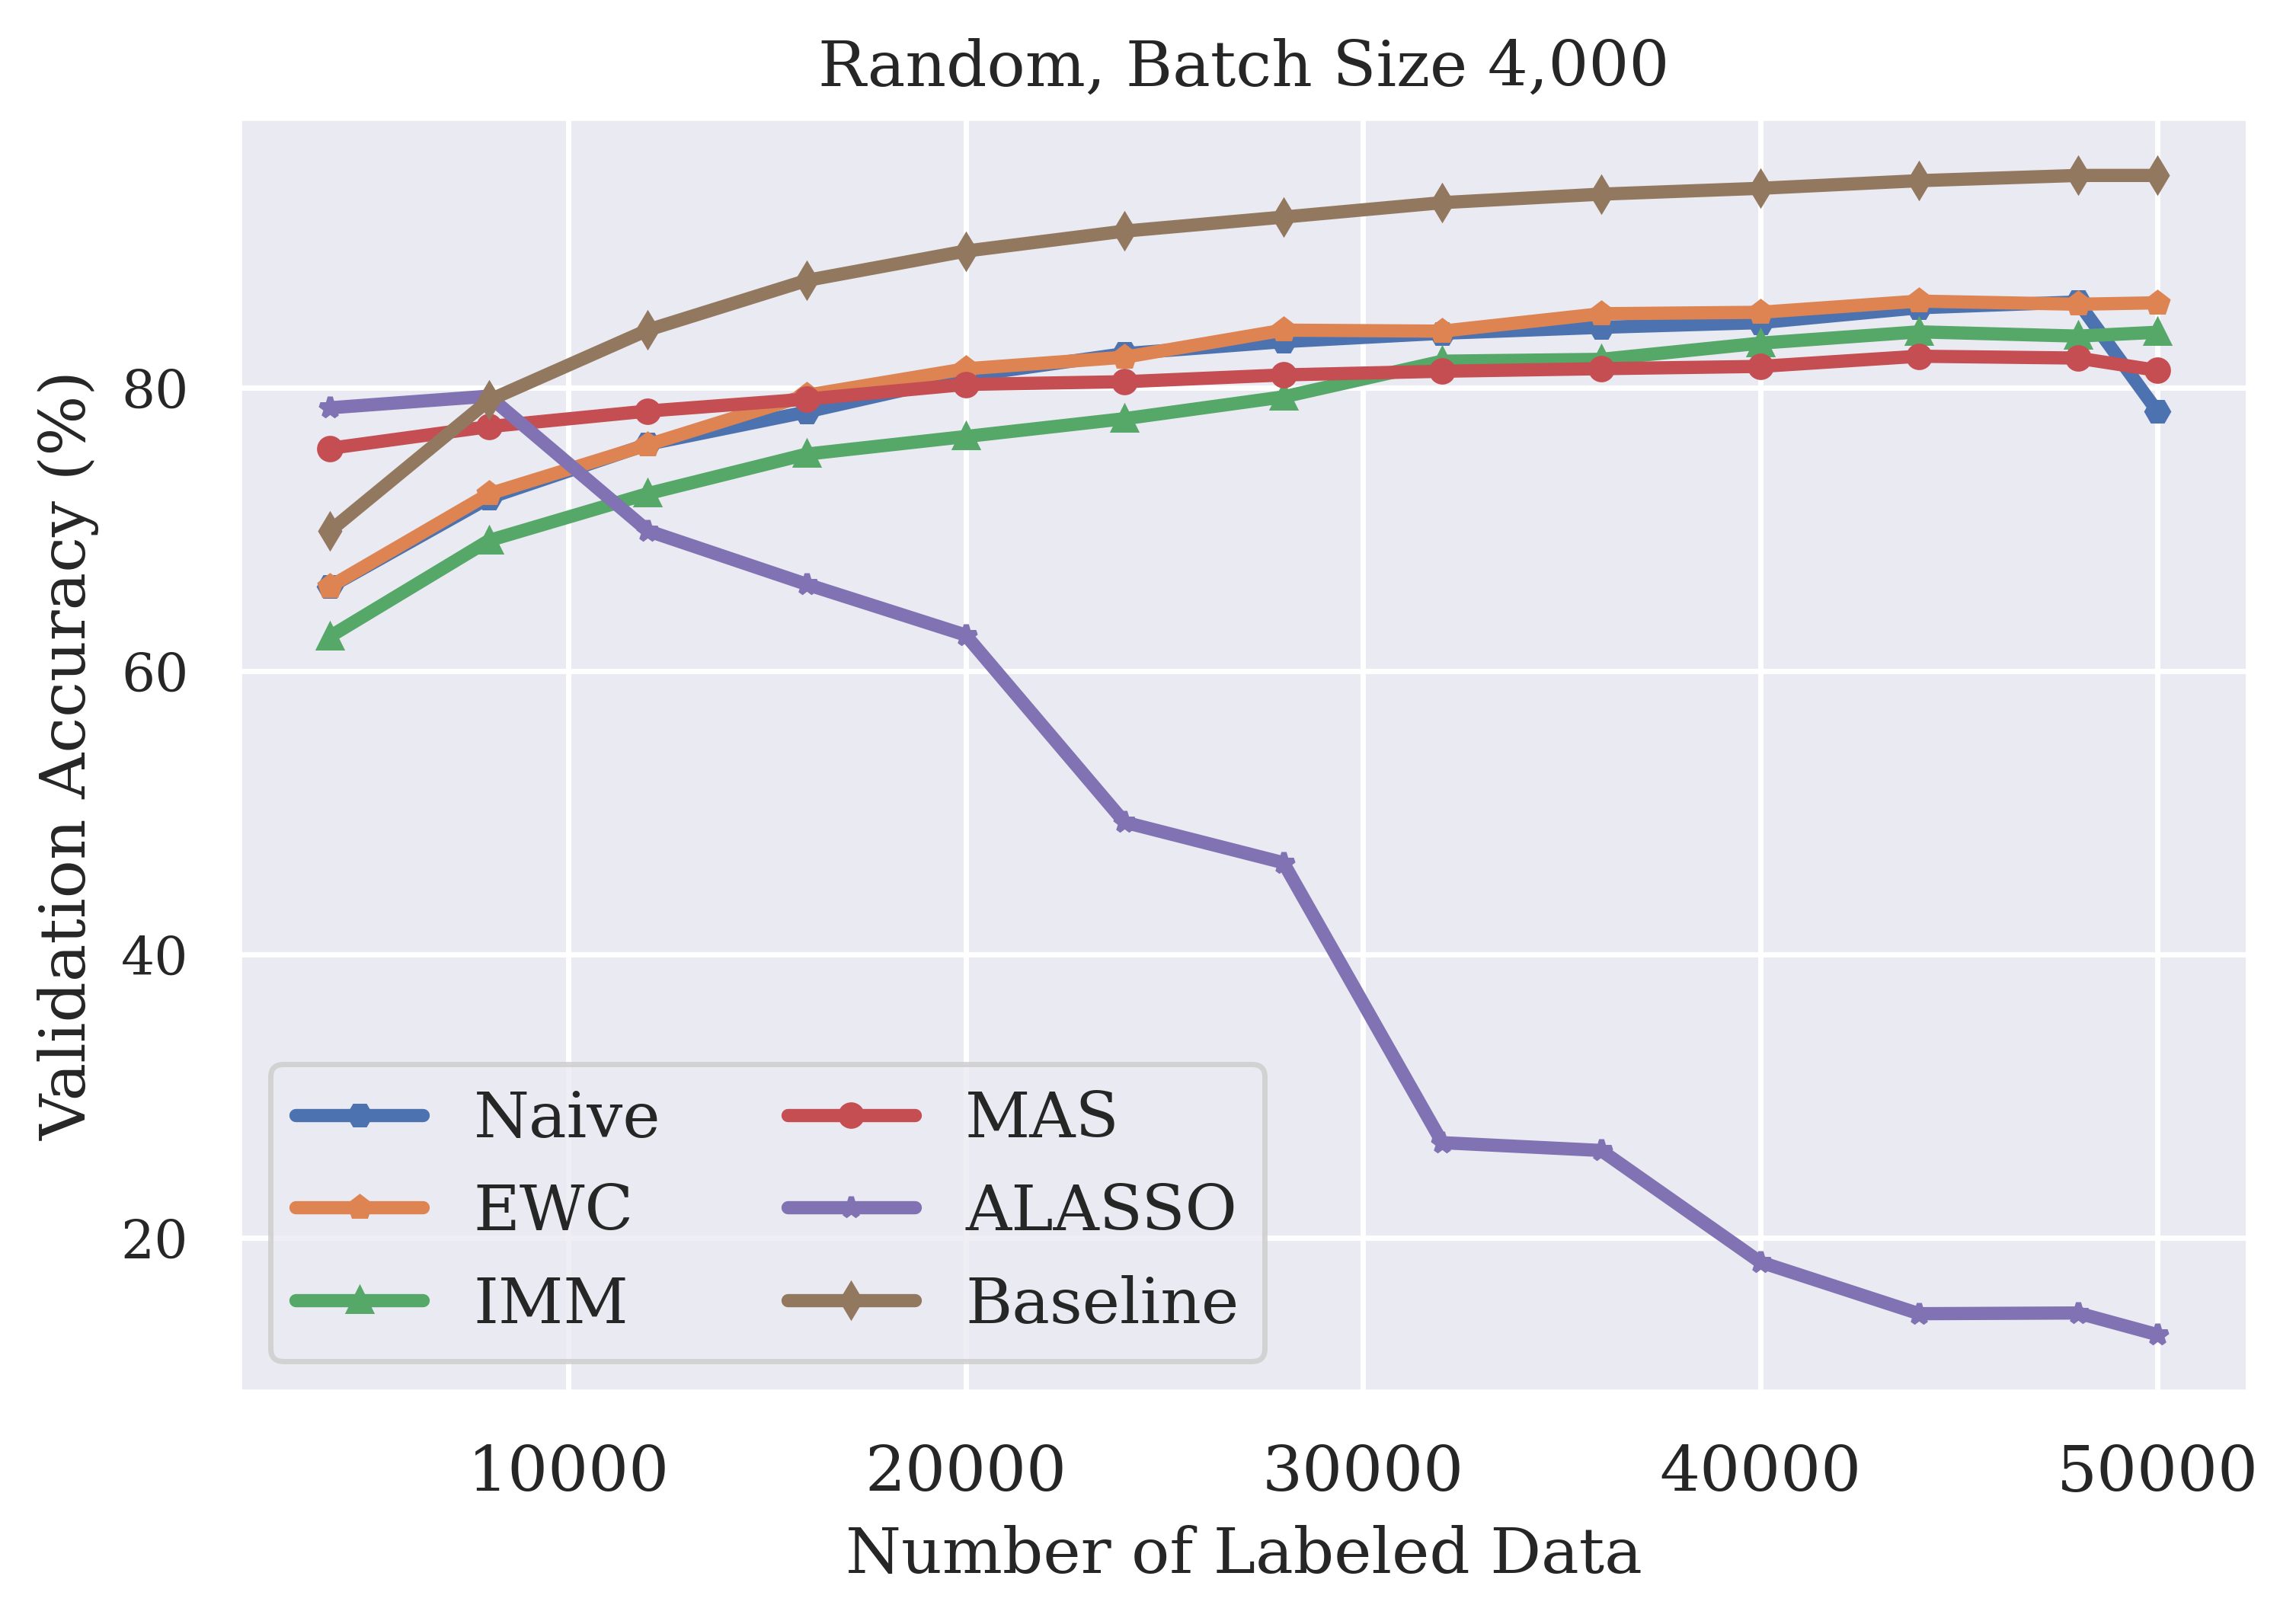
\includegraphics[width=0.32\linewidth]{images/results_CAL/random_4000b_acc.png} \hfill
    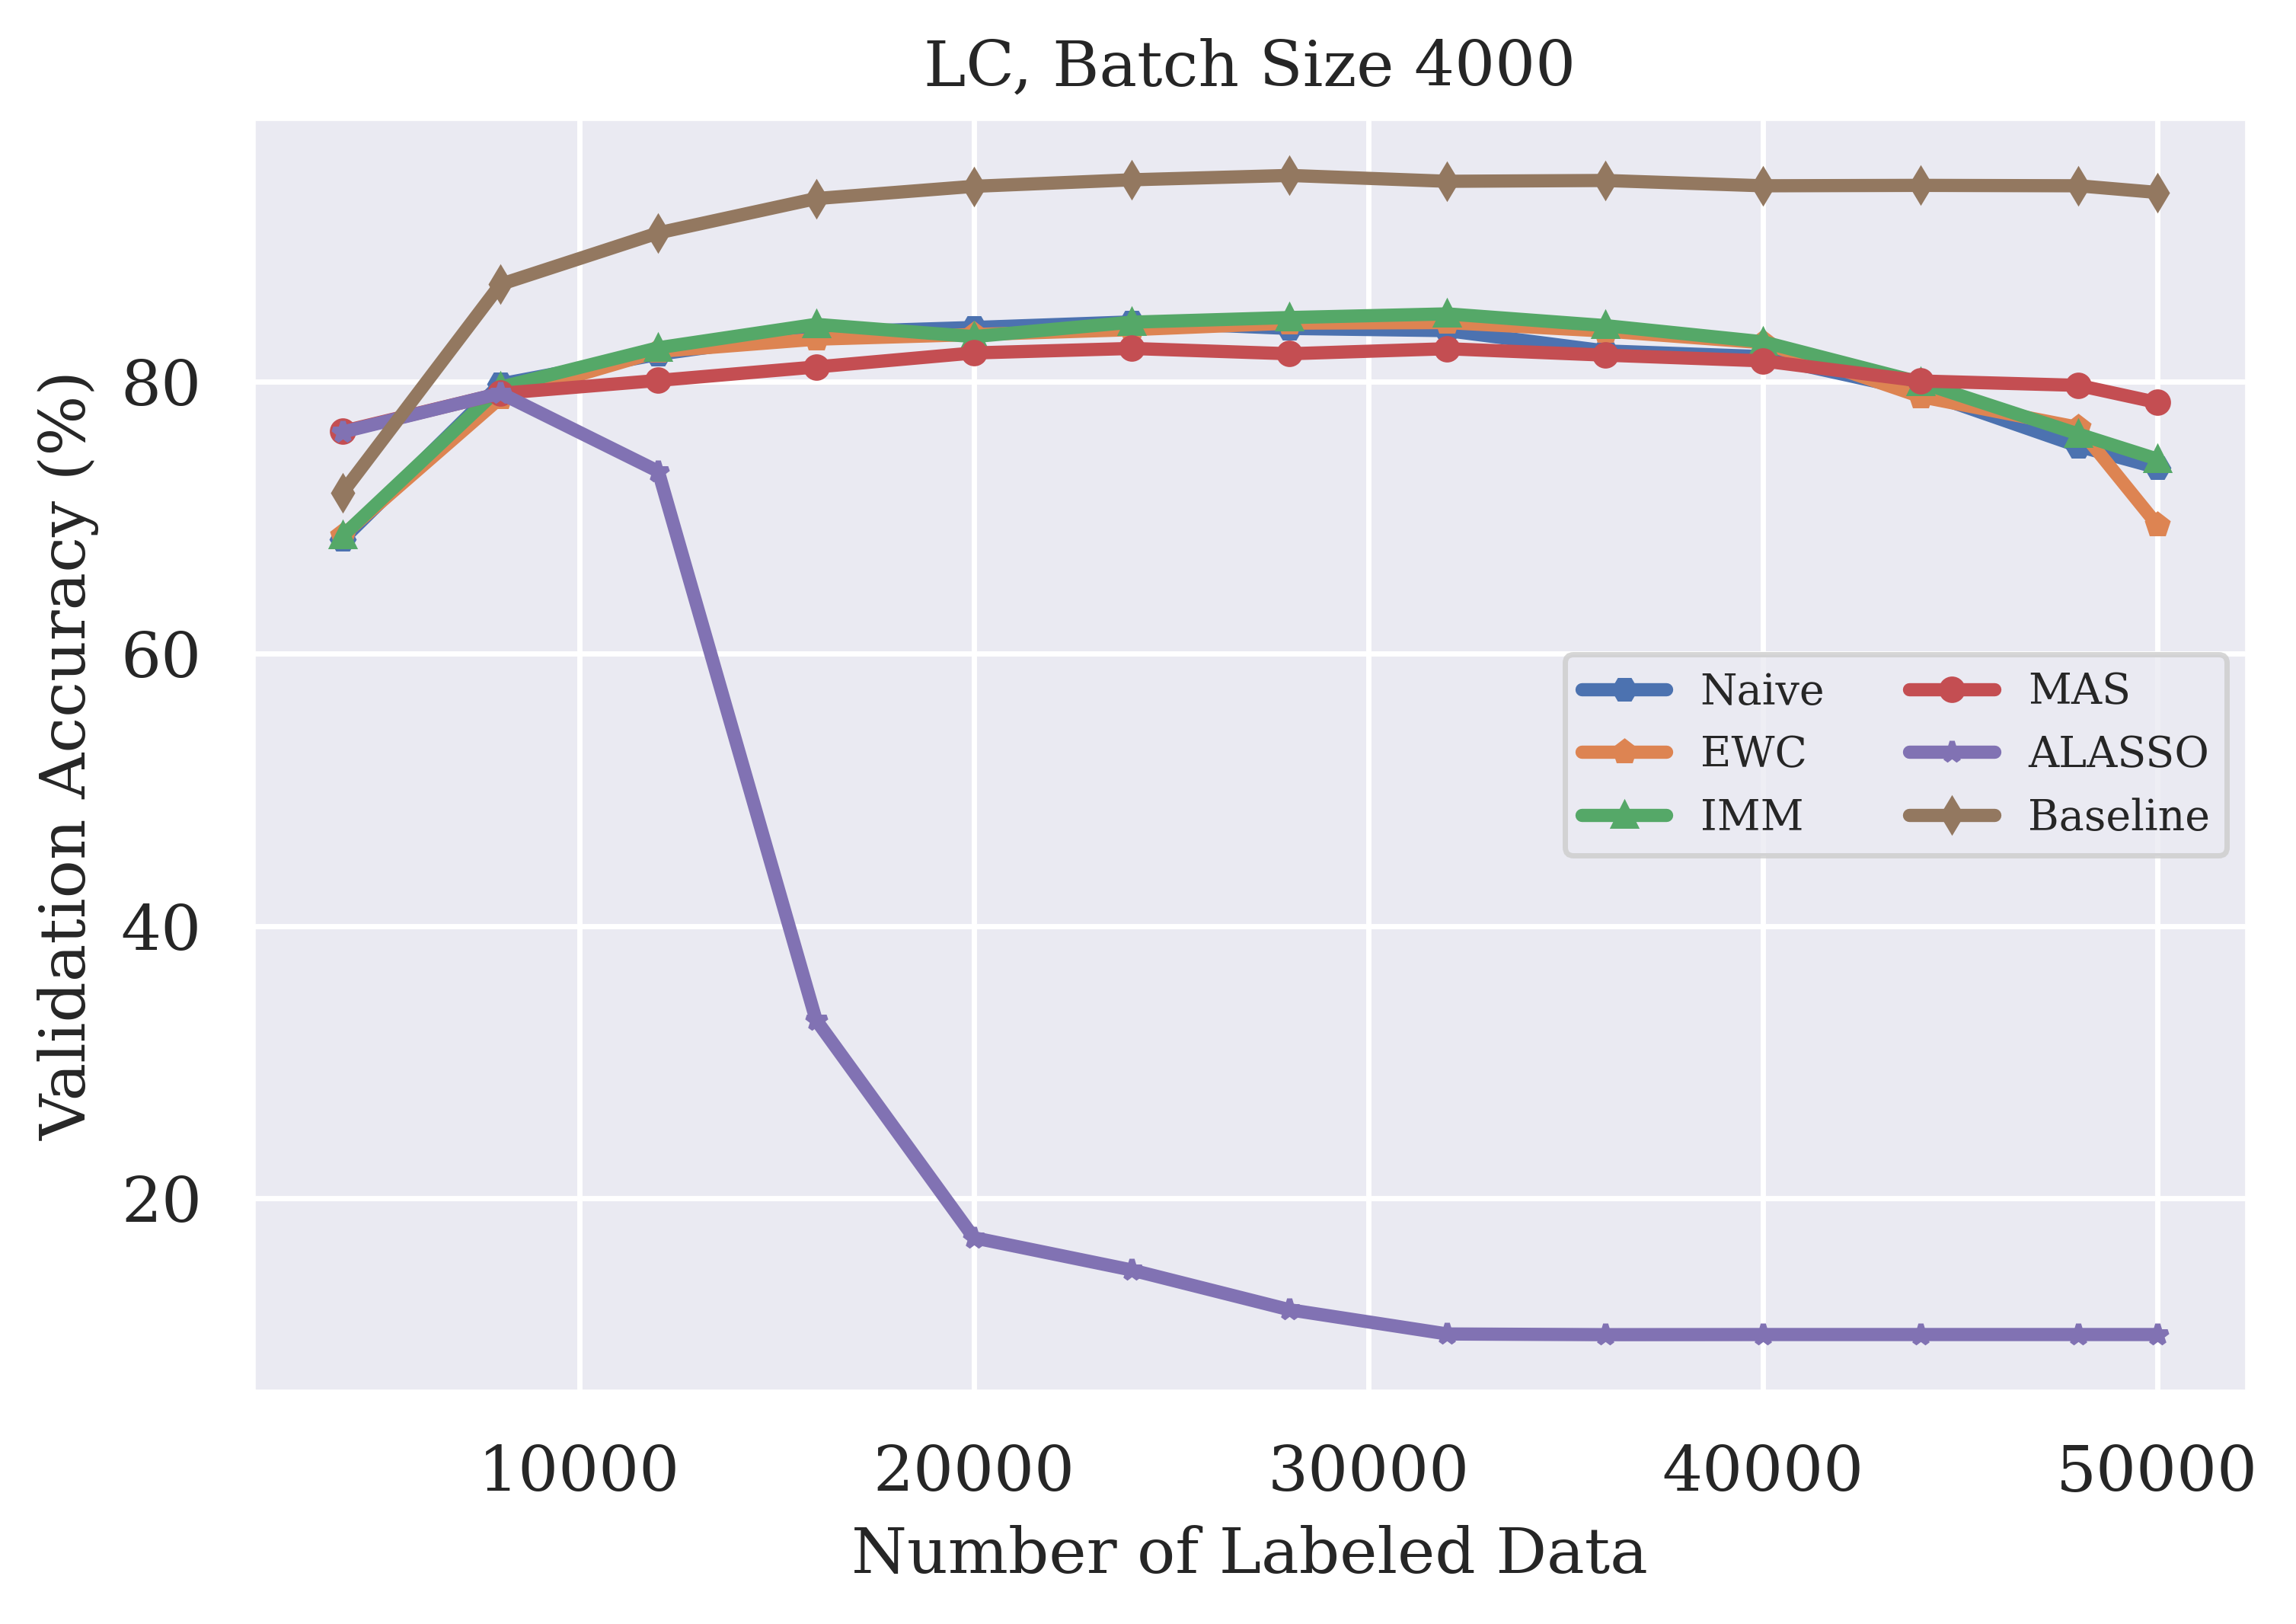
\includegraphics[width=0.32\linewidth]{images/results_CAL/lc_4000b_acc.png} \hfill
    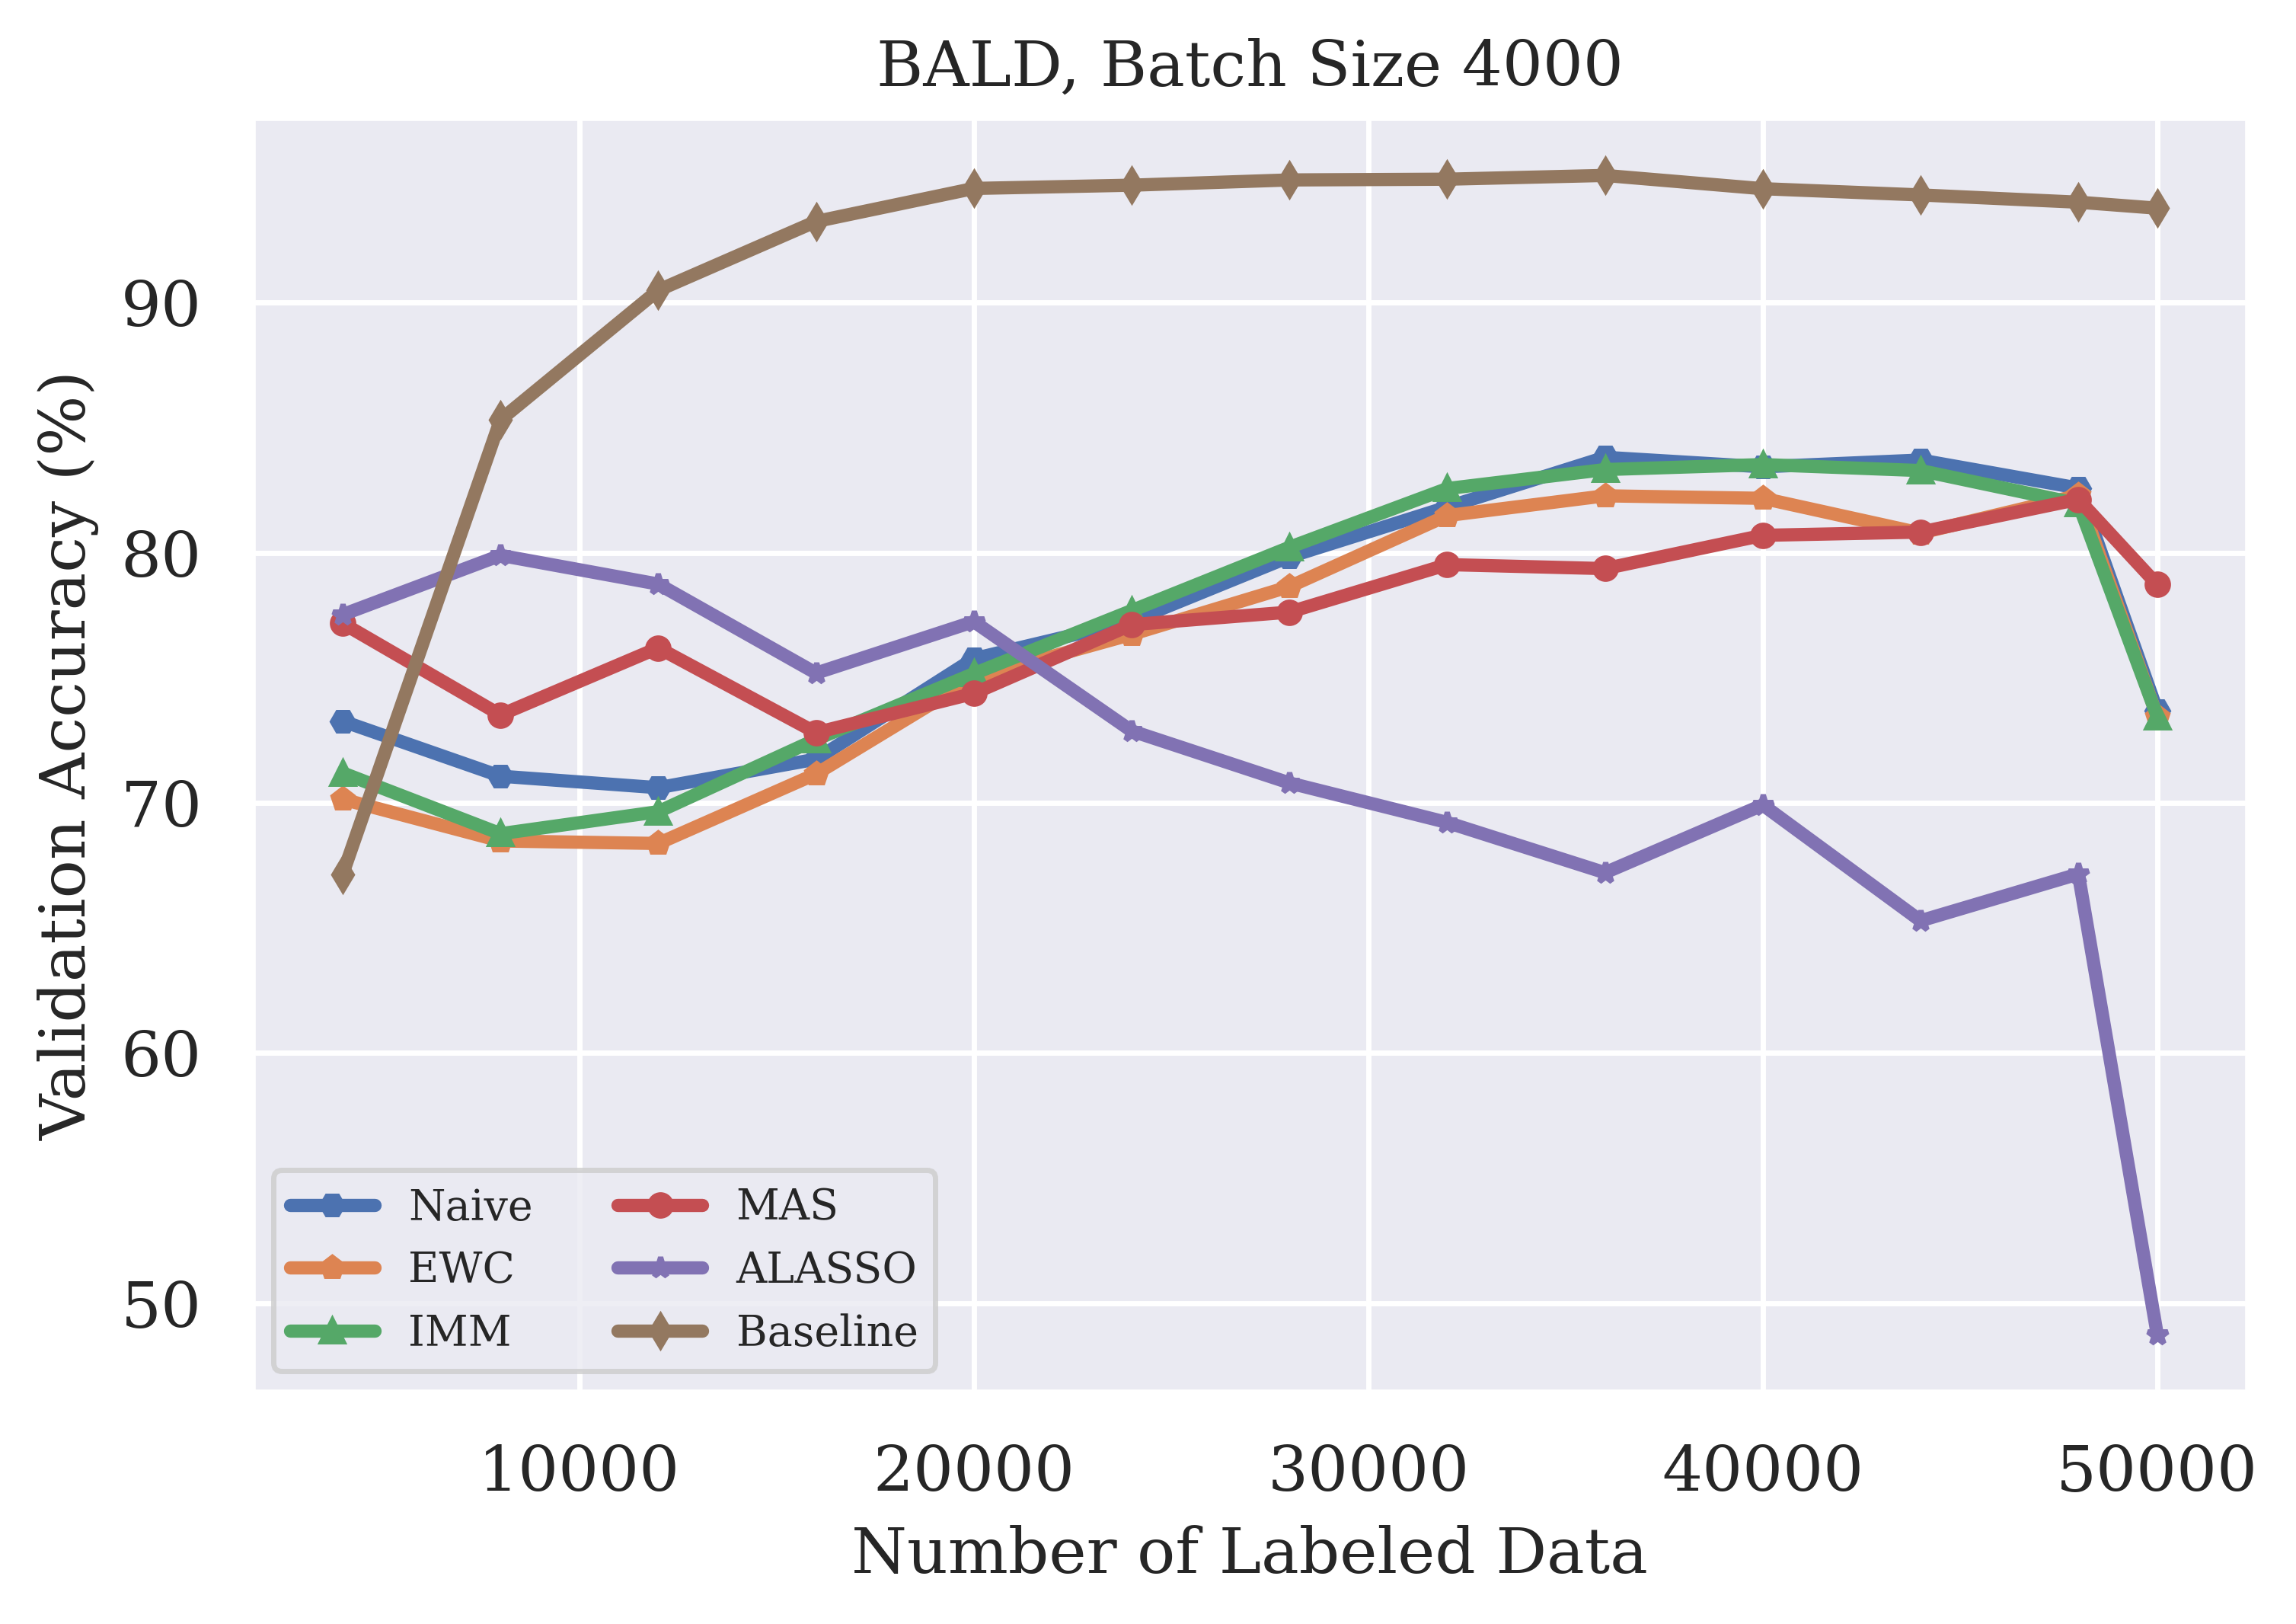
\includegraphics[width=0.32\linewidth]{images/results_CAL/bald_4000b_acc.png}
    \\[\smallskipamount]
    \hfill 
    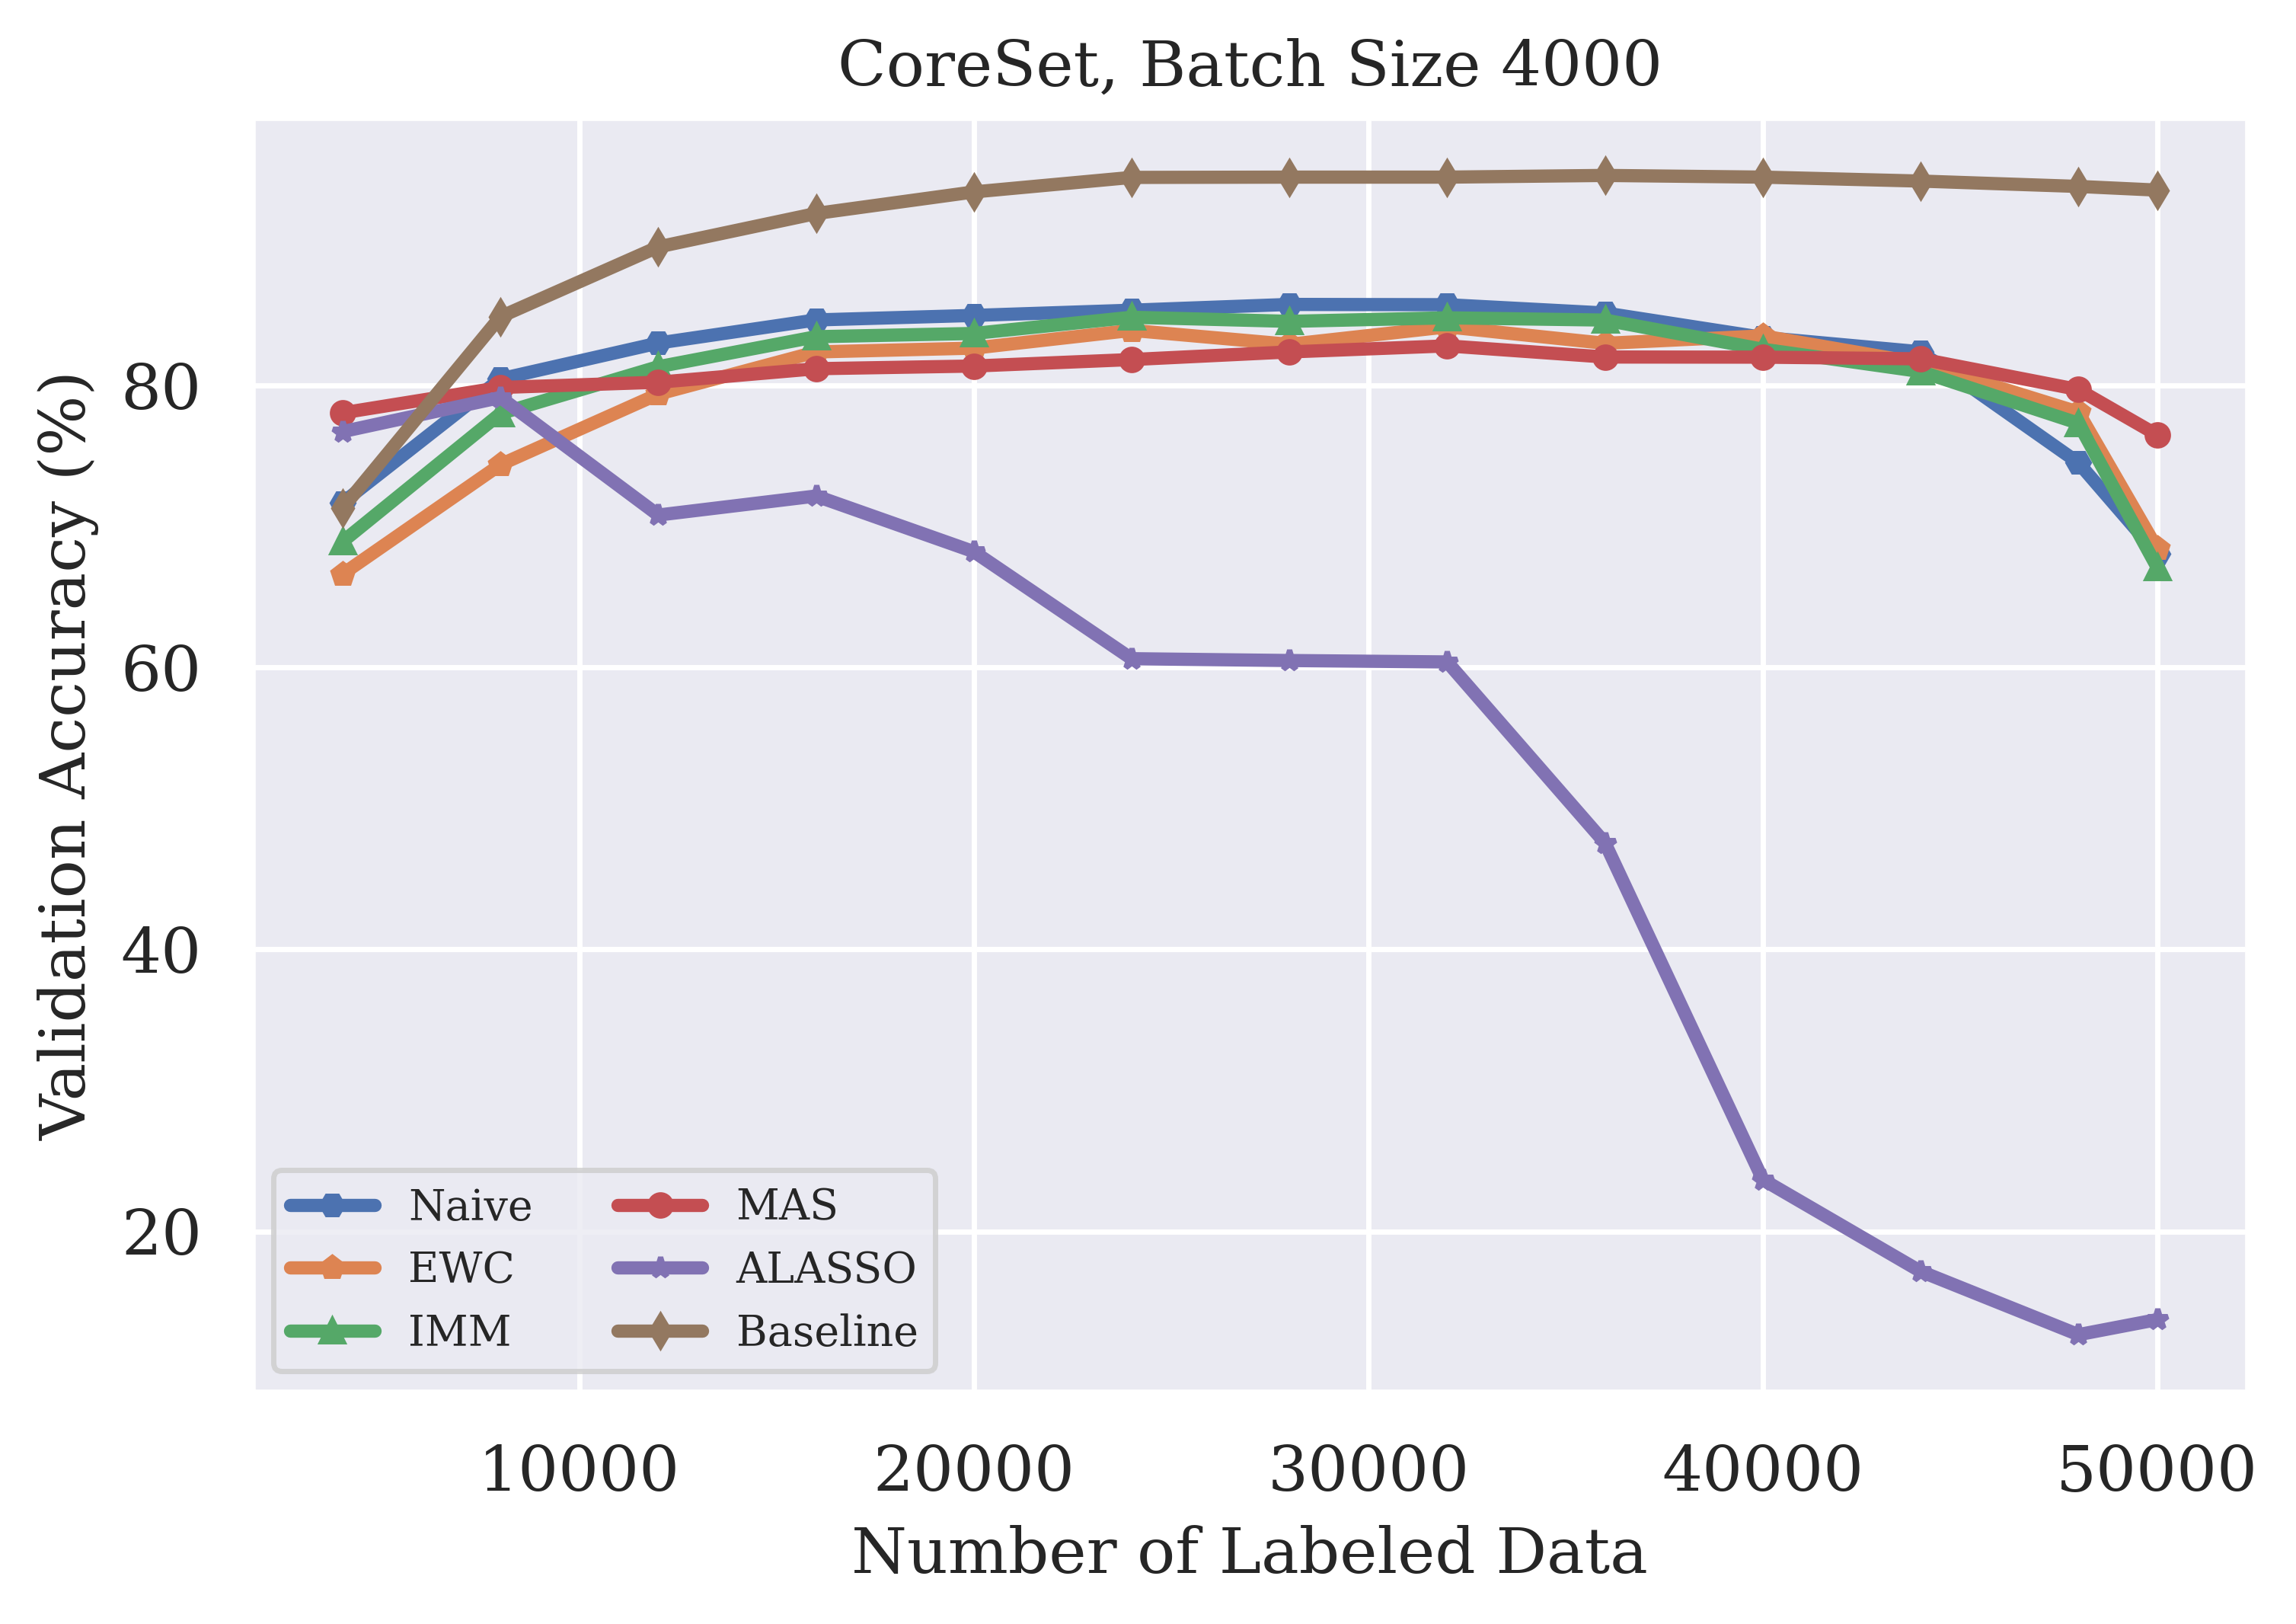
\includegraphics[width=0.32\linewidth]{images/results_CAL/coreset_4000b_acc.png} \hfill
    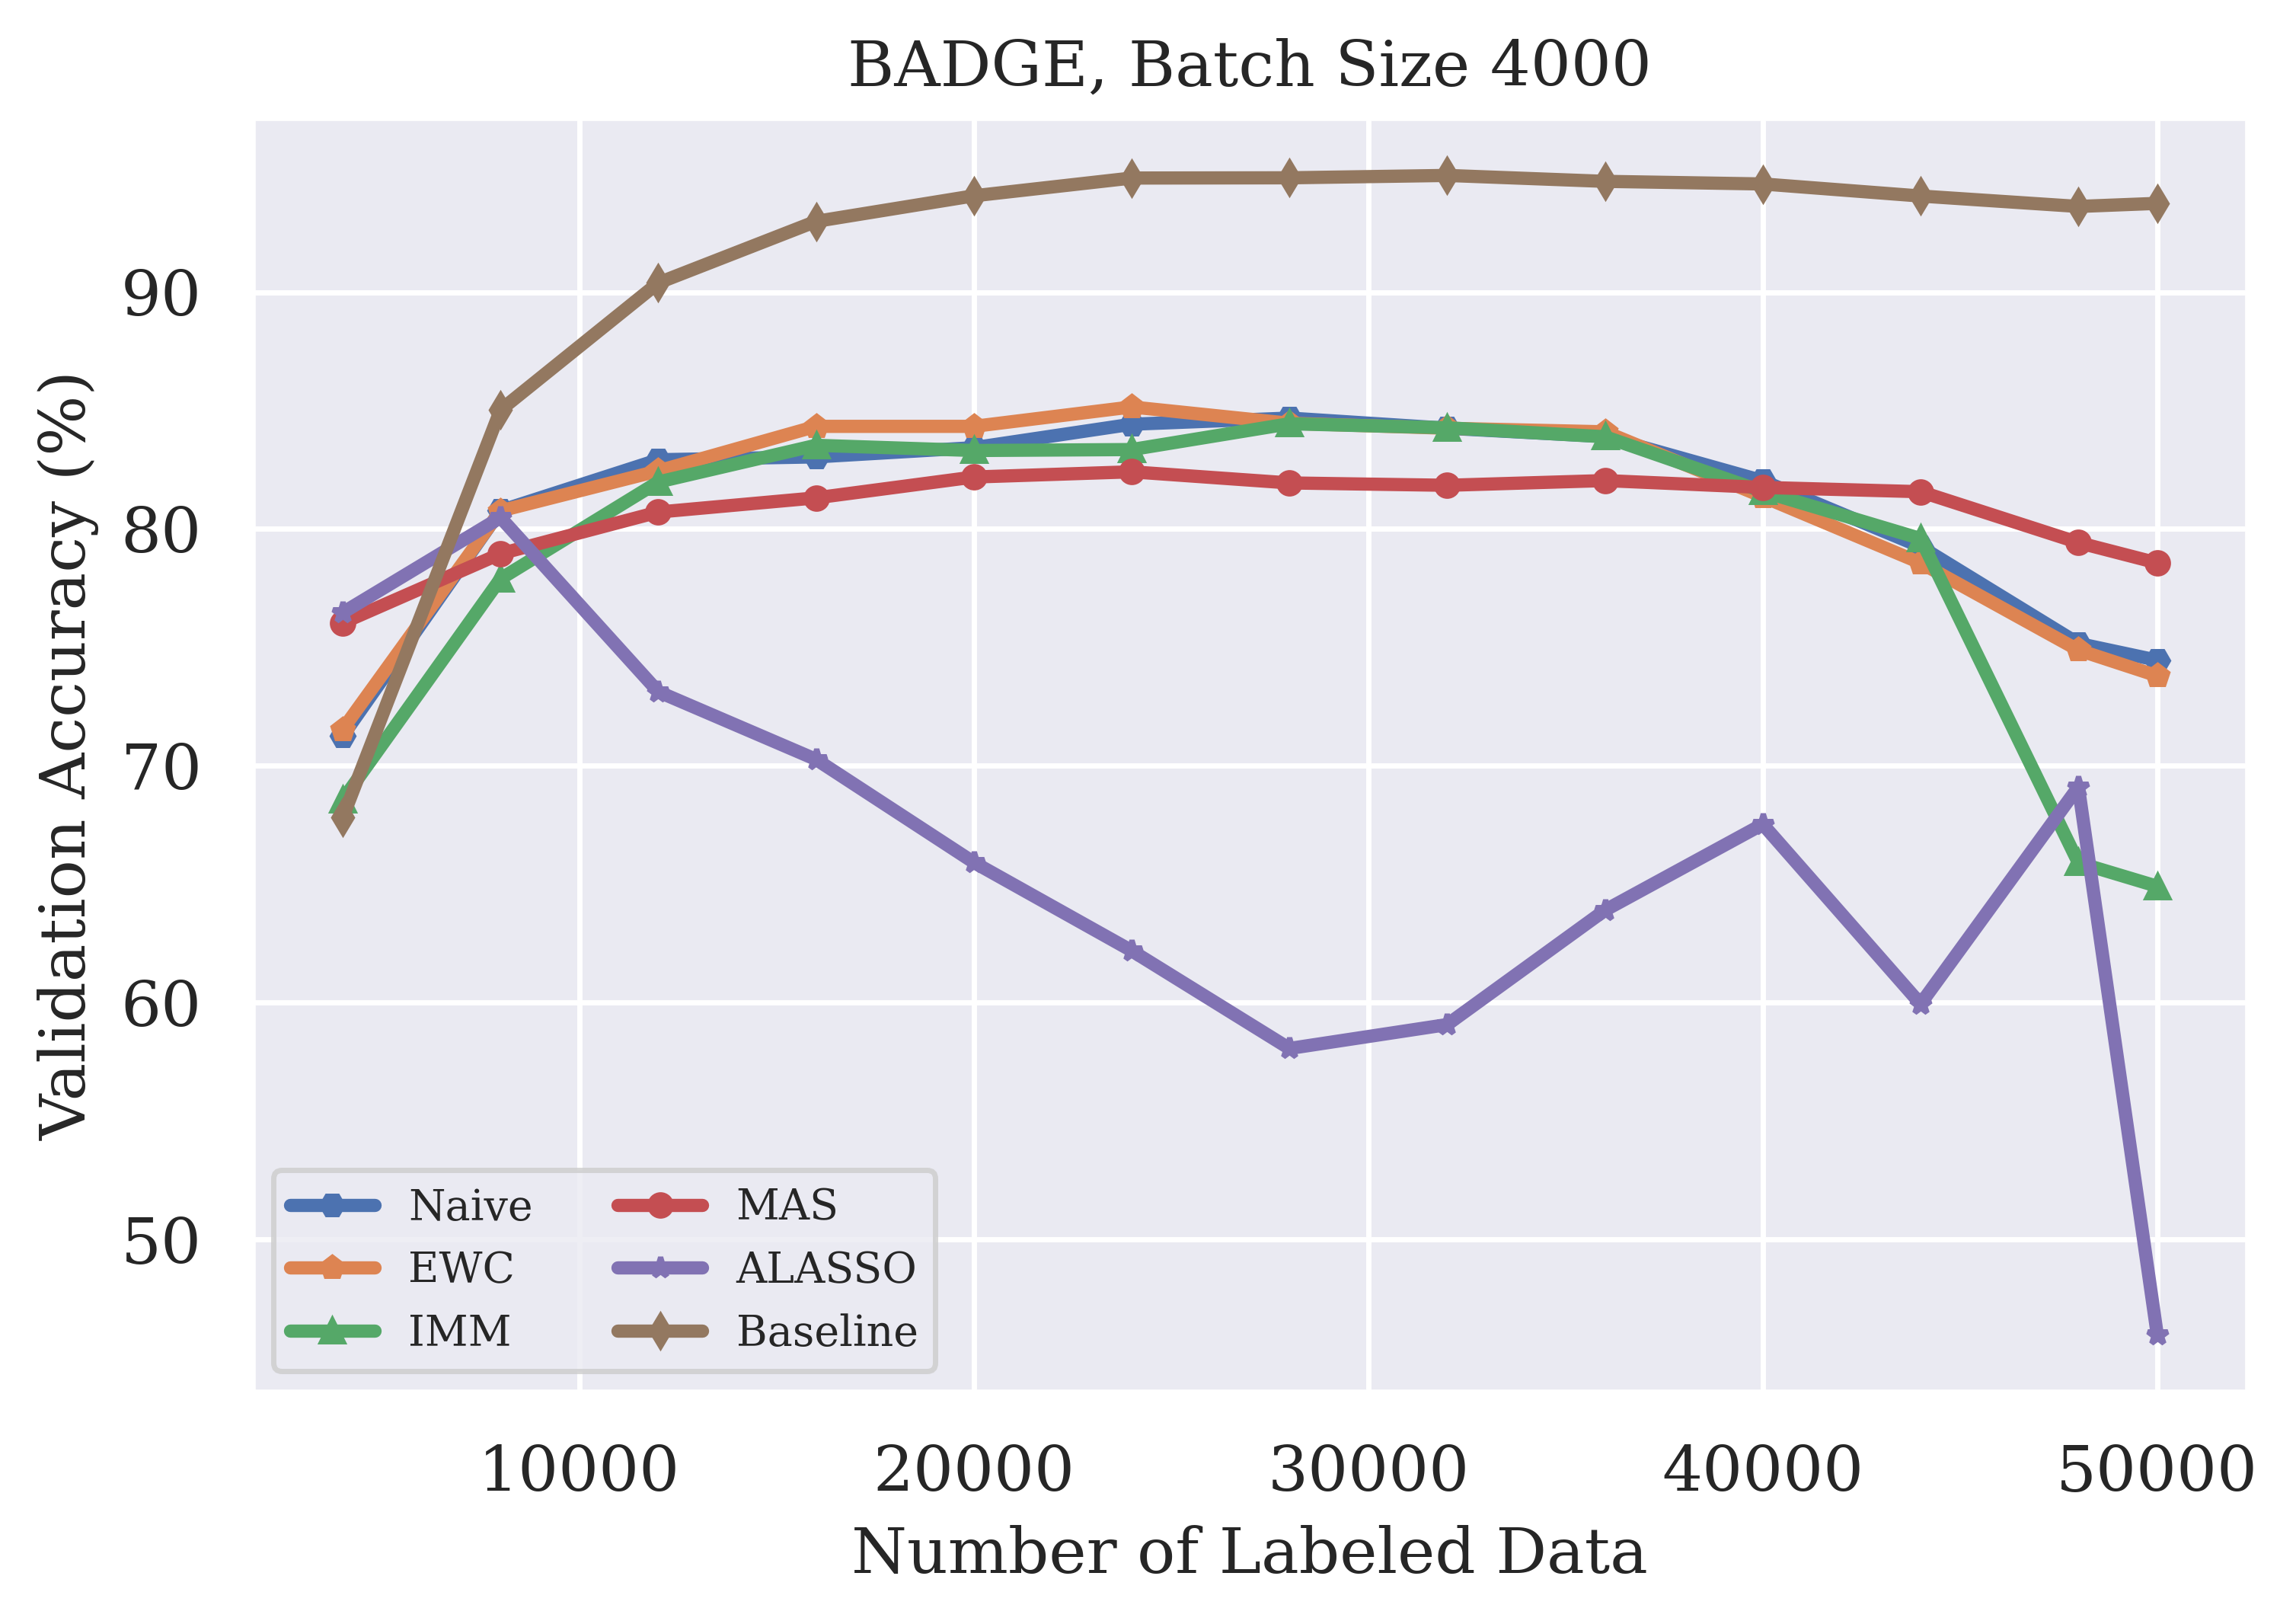
\includegraphics[width=0.32\linewidth]{images/results_CAL/badge_4000b_acc.png} \hfill
    \caption[Continual Active Learning with \gls{badge} with varying batch size]{Comparison of validation accuracy of regularization-based continual learning strategies
    with batch size 4000.}
    \label{fig:Evaluation:CAL:4000bAcc}
\end{figure}




% \begin{figure}[h]
%     \centering
%     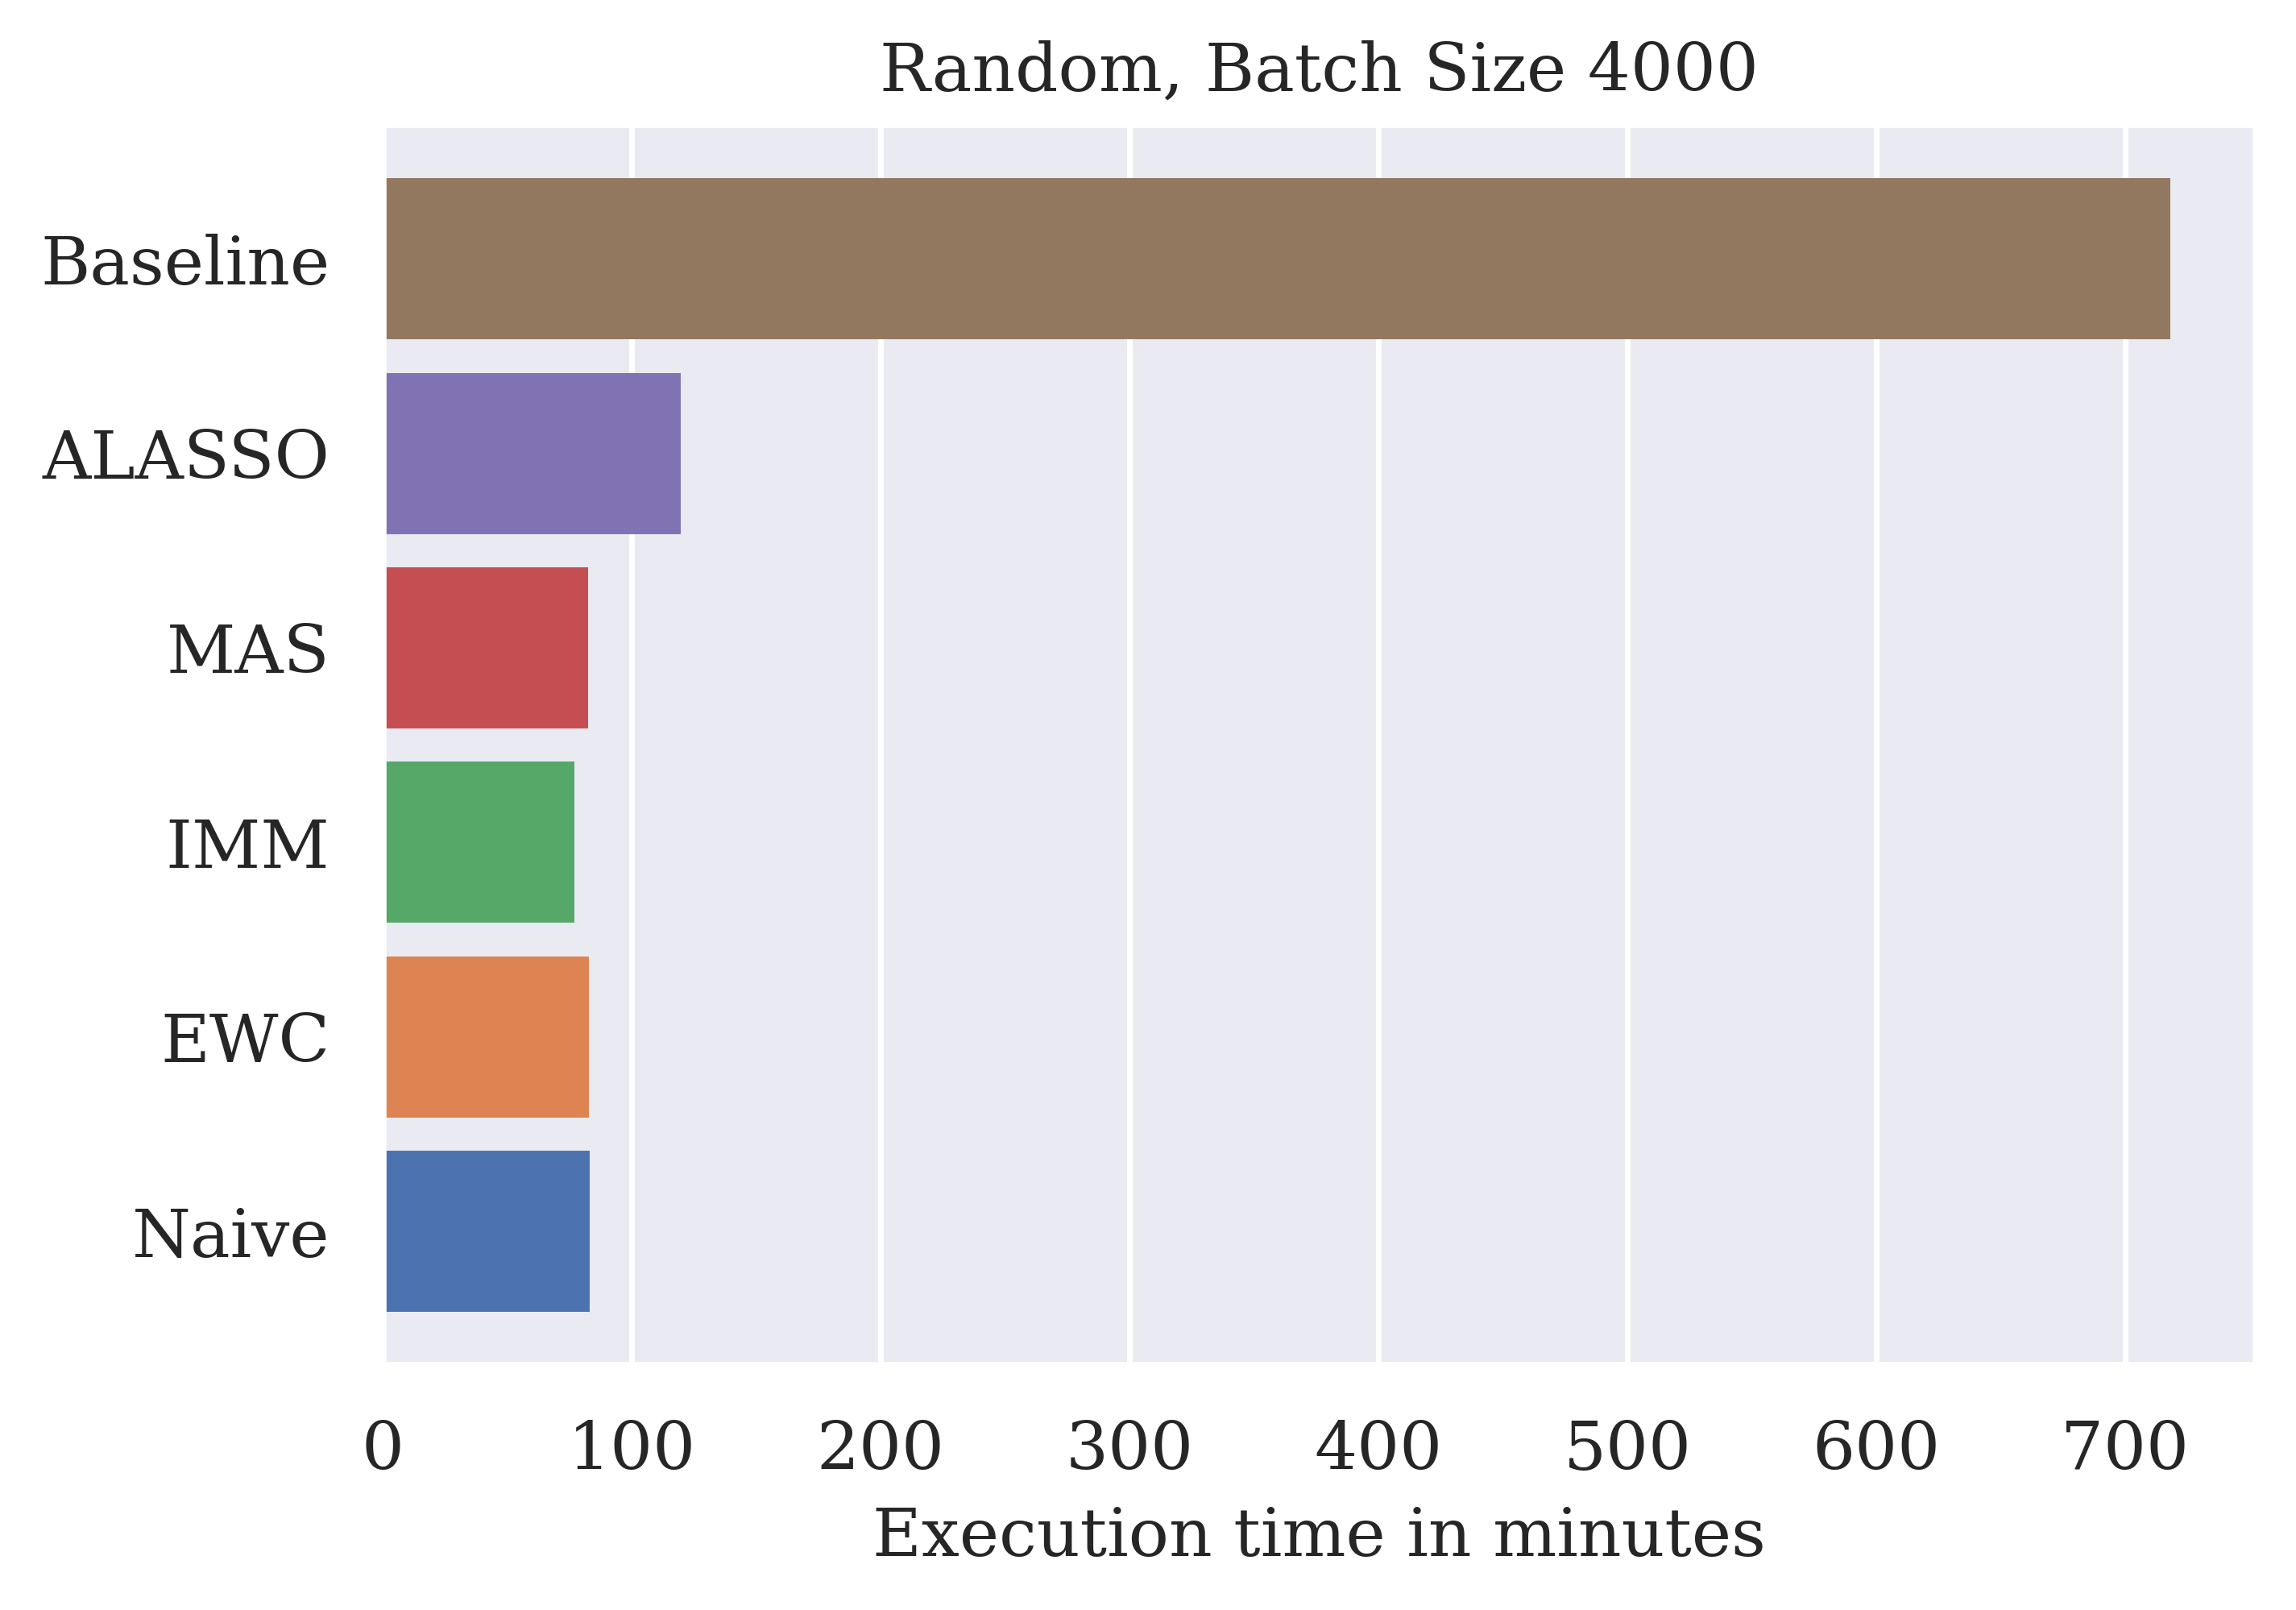
\includegraphics[width=0.32\linewidth]{images/results_CAL/random_4000b_time.png} \hfill
%     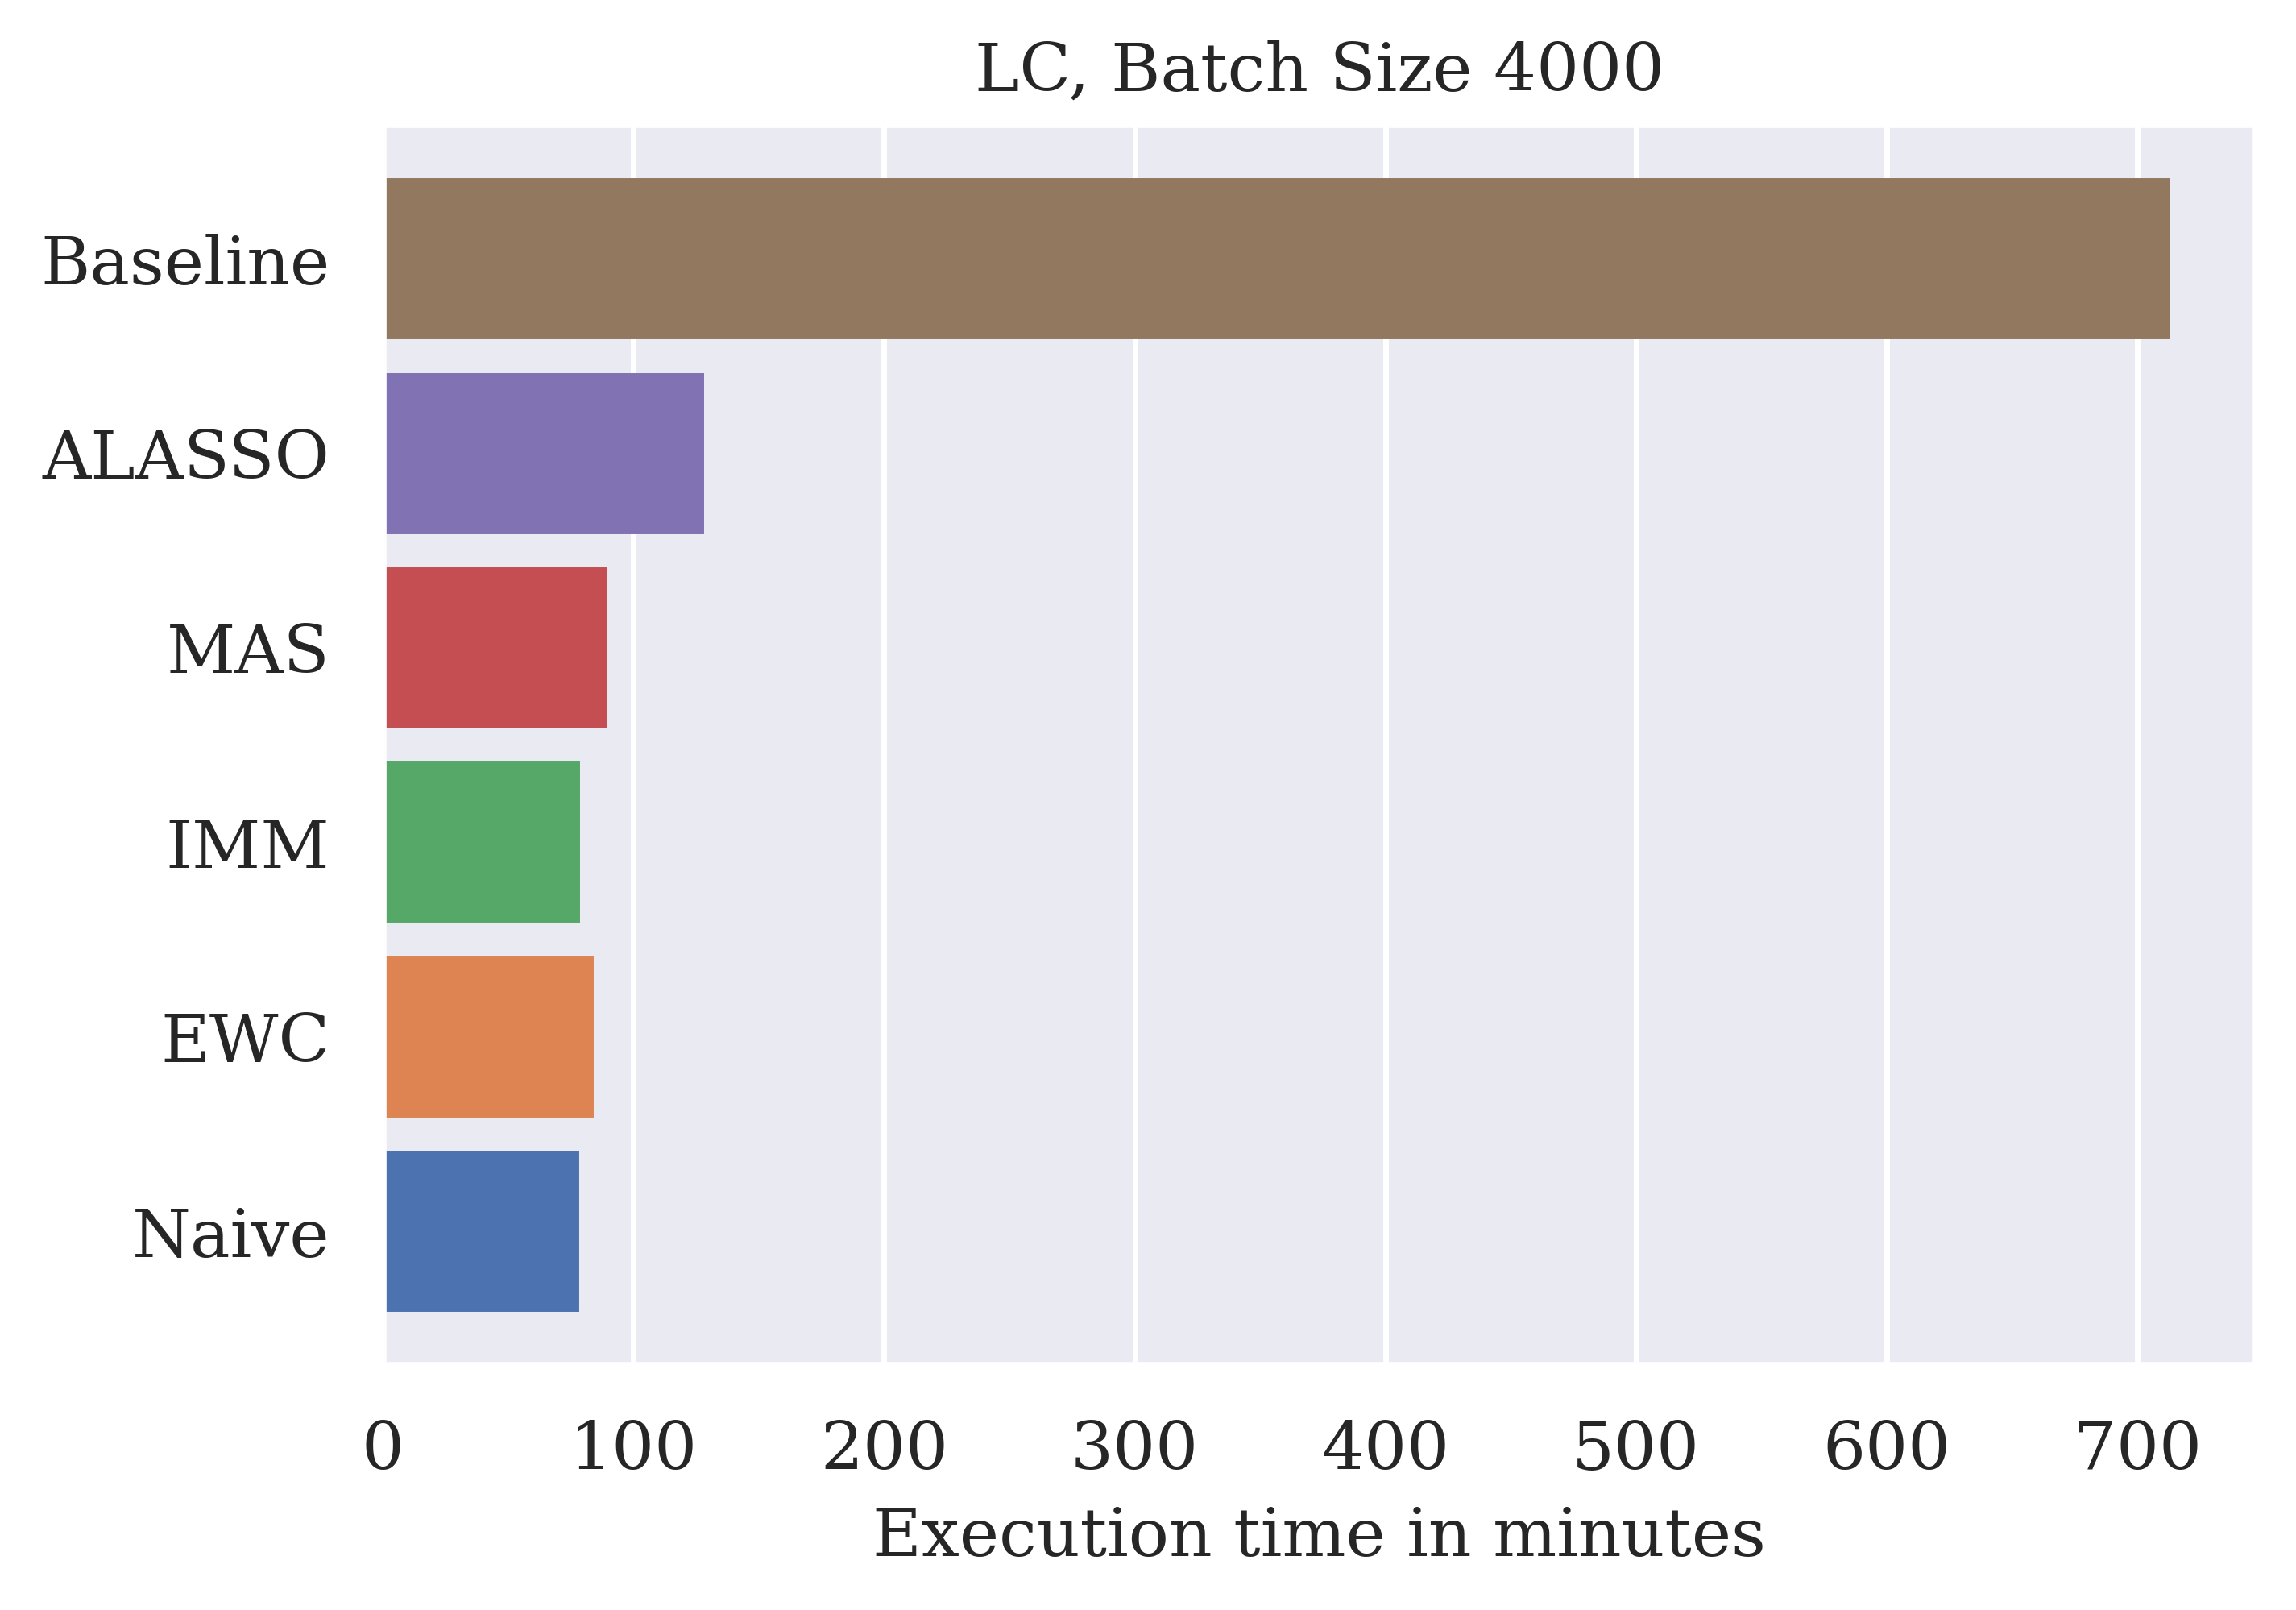
\includegraphics[width=0.32\linewidth]{images/results_CAL/lc_4000b_time.png} \hfill
%     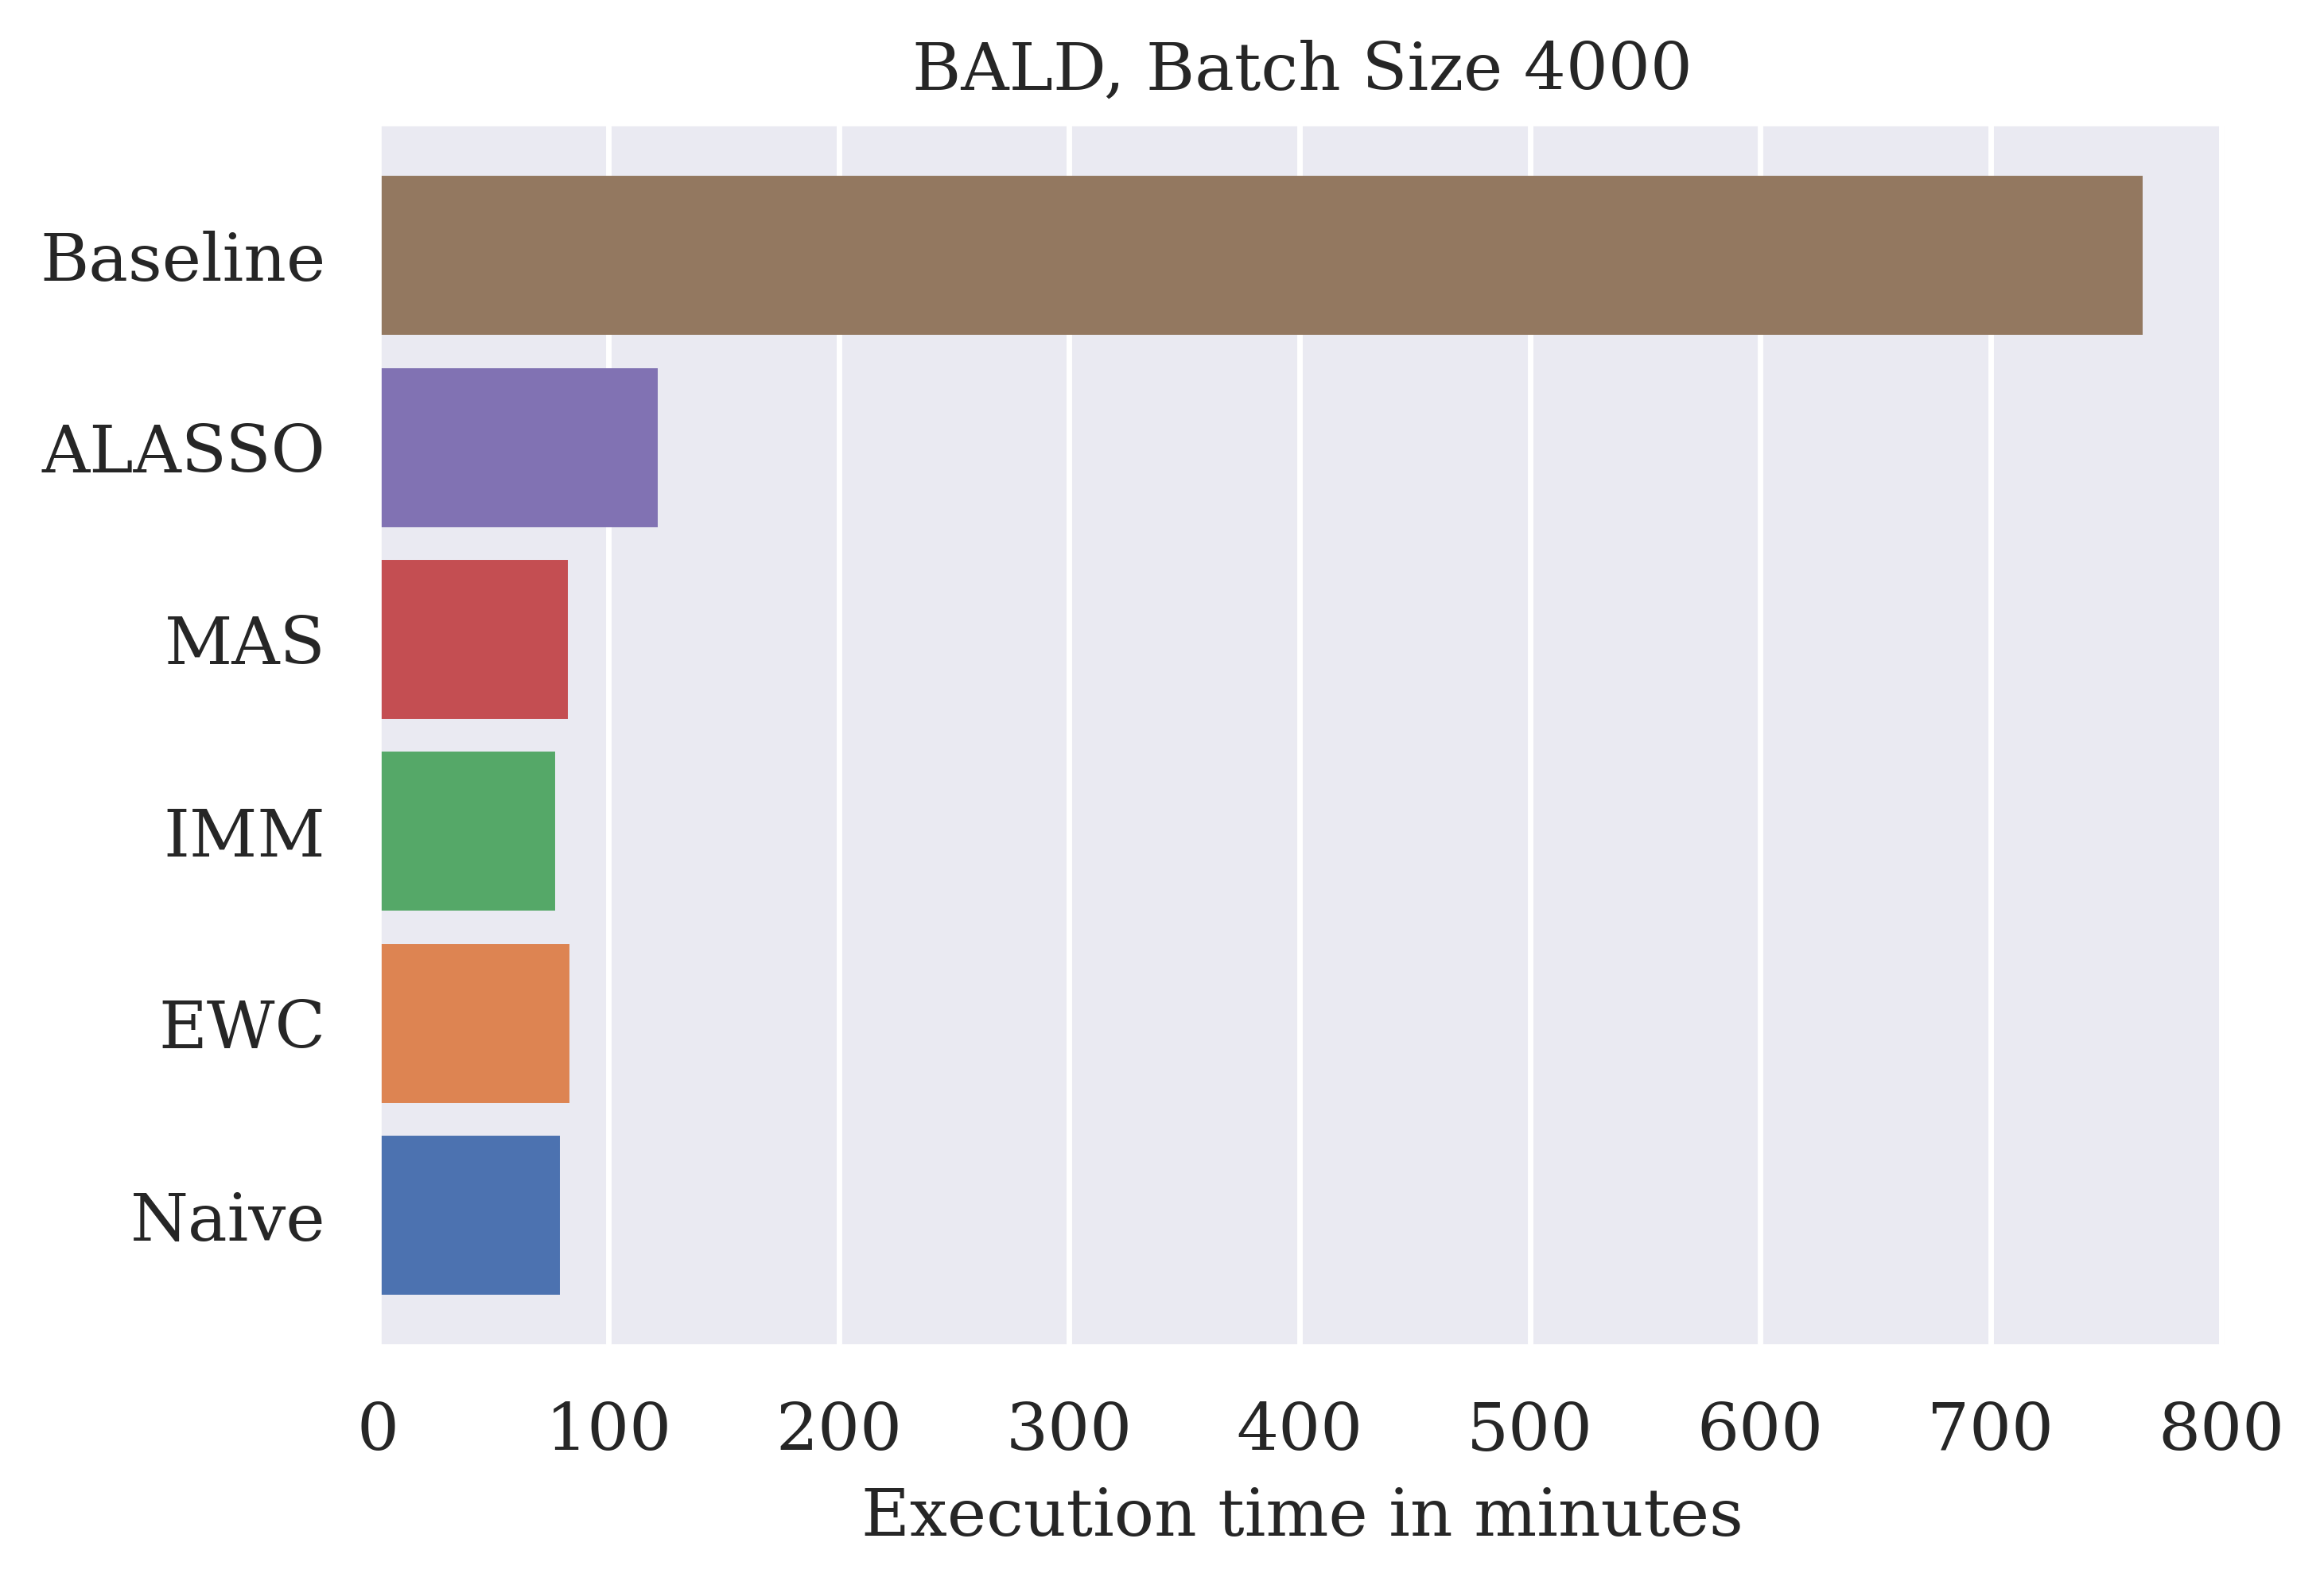
\includegraphics[width=0.32\linewidth]{images/results_CAL/bald_4000b_time.png}
%     \\[\smallskipamount]
%     \hfill 
%     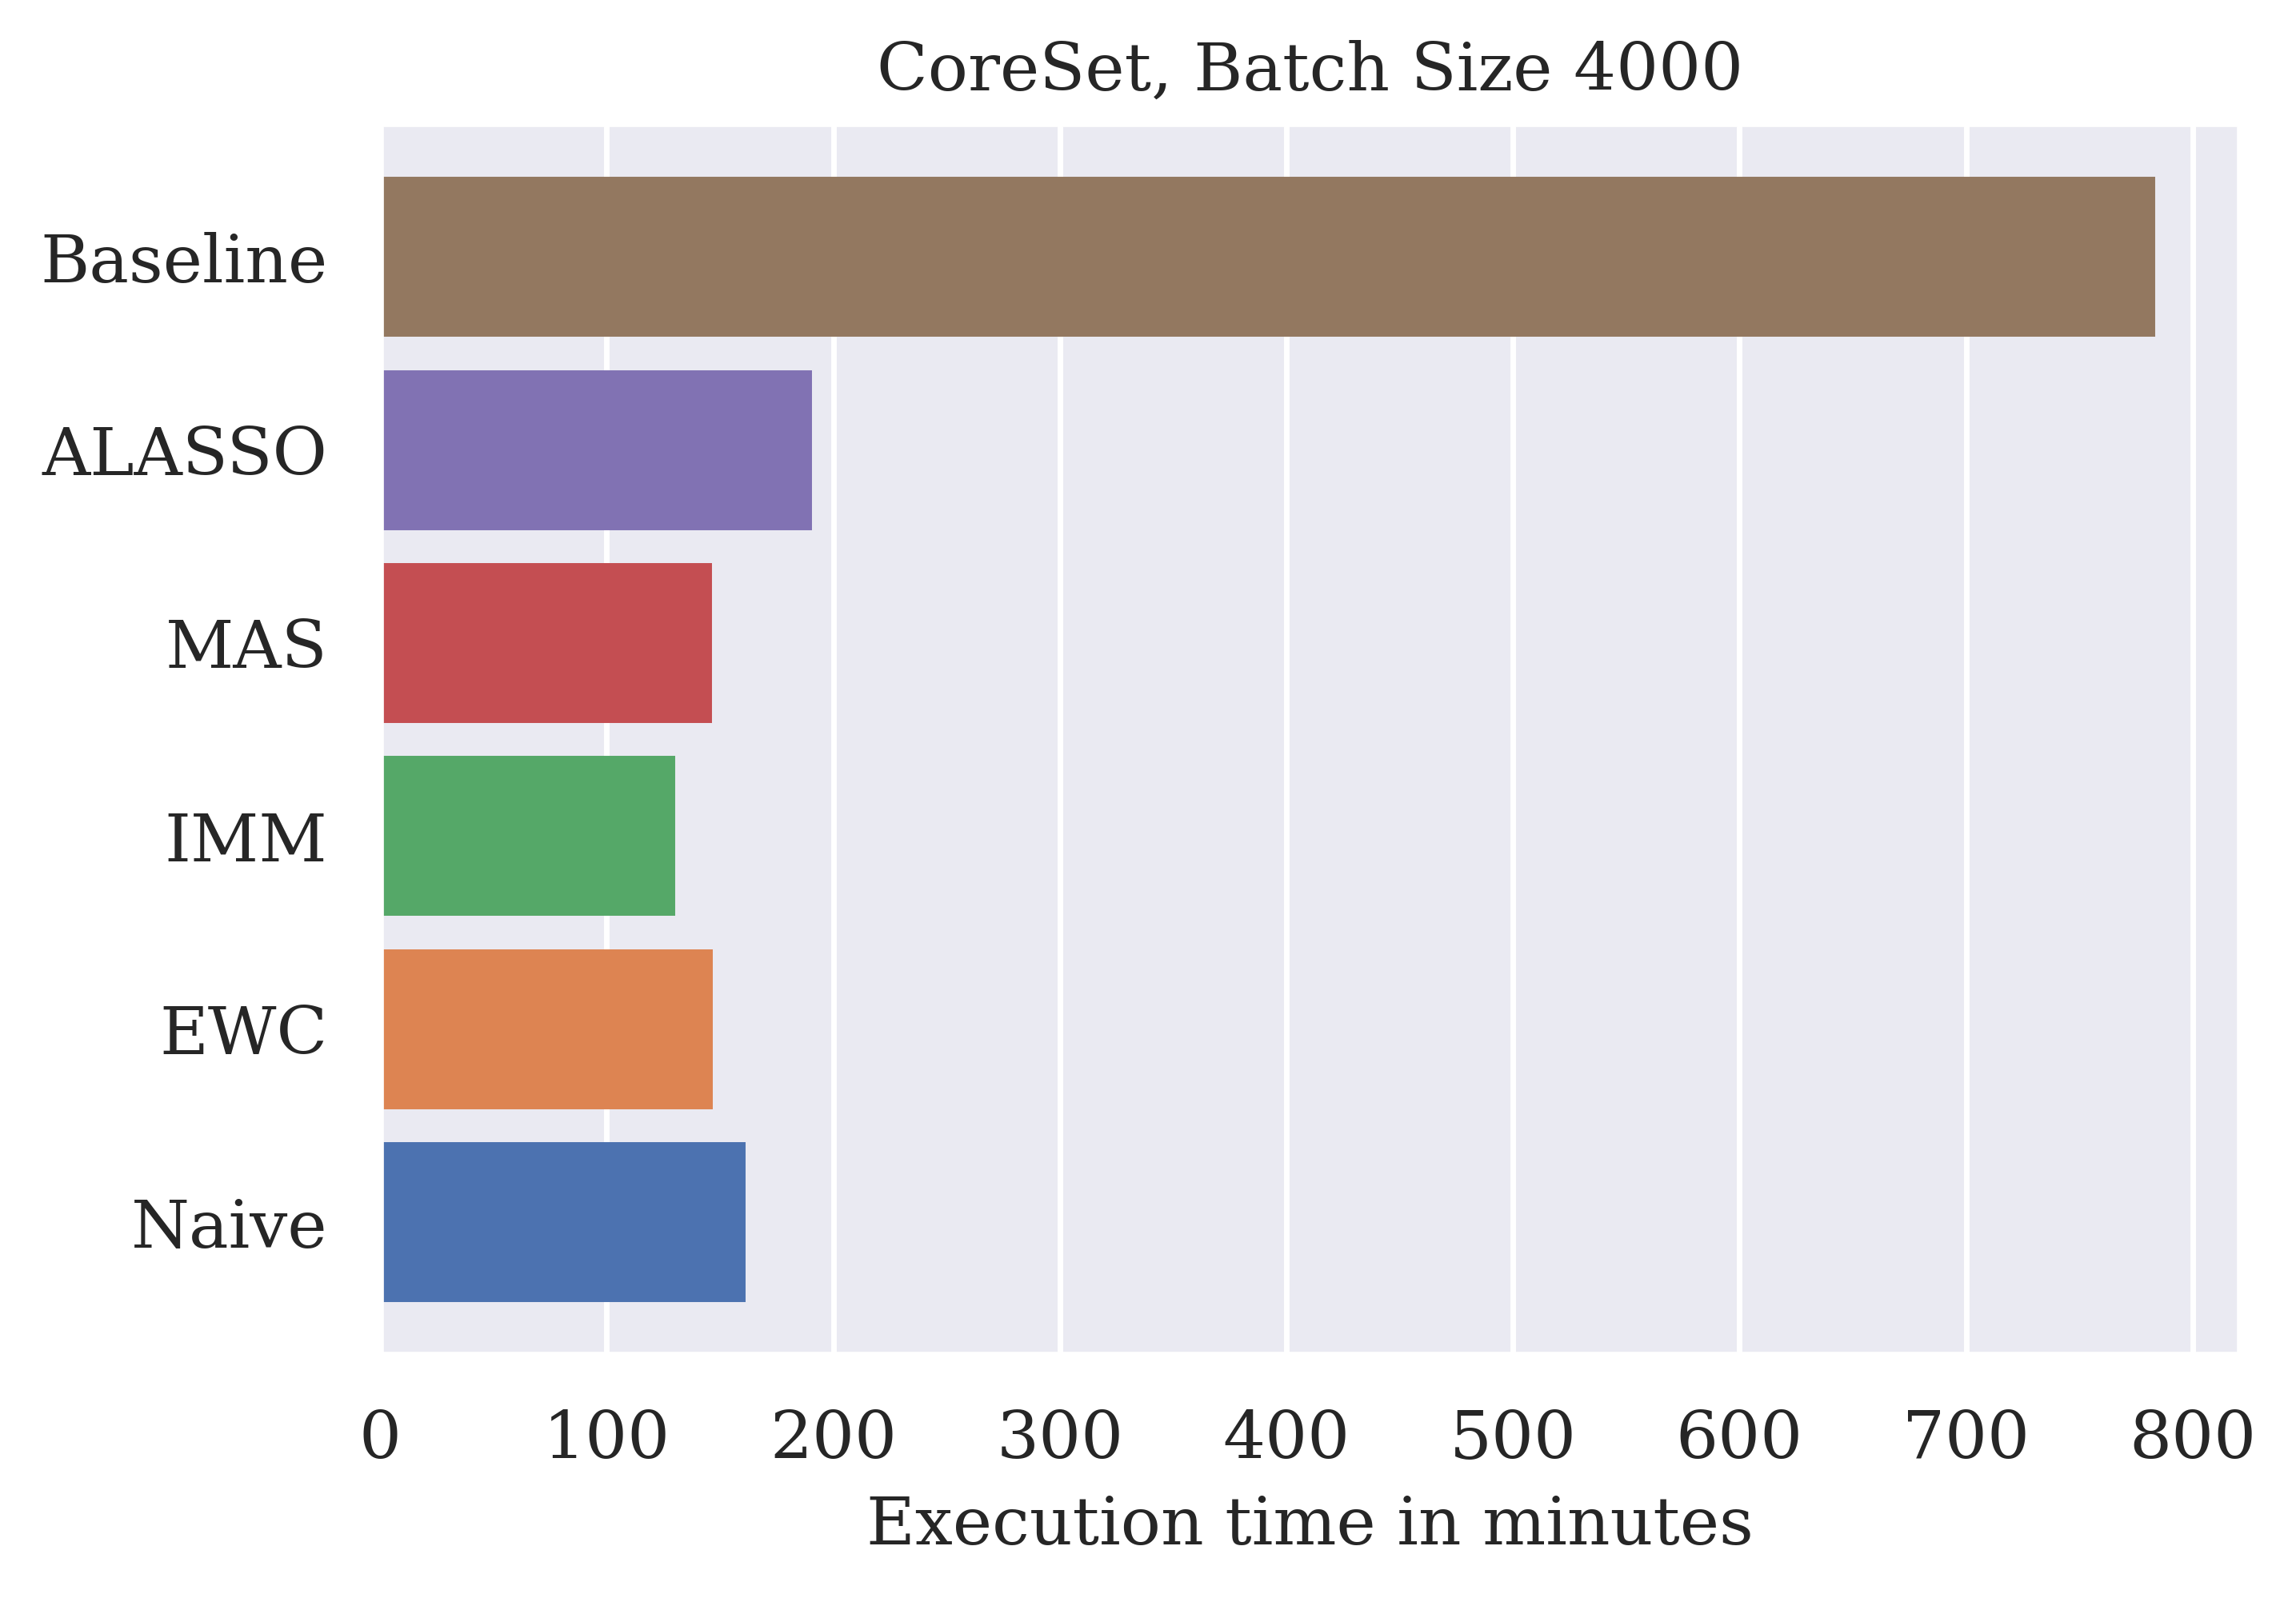
\includegraphics[width=0.32\linewidth]{images/results_CAL/coreset_4000b_time.png} \hfill
%     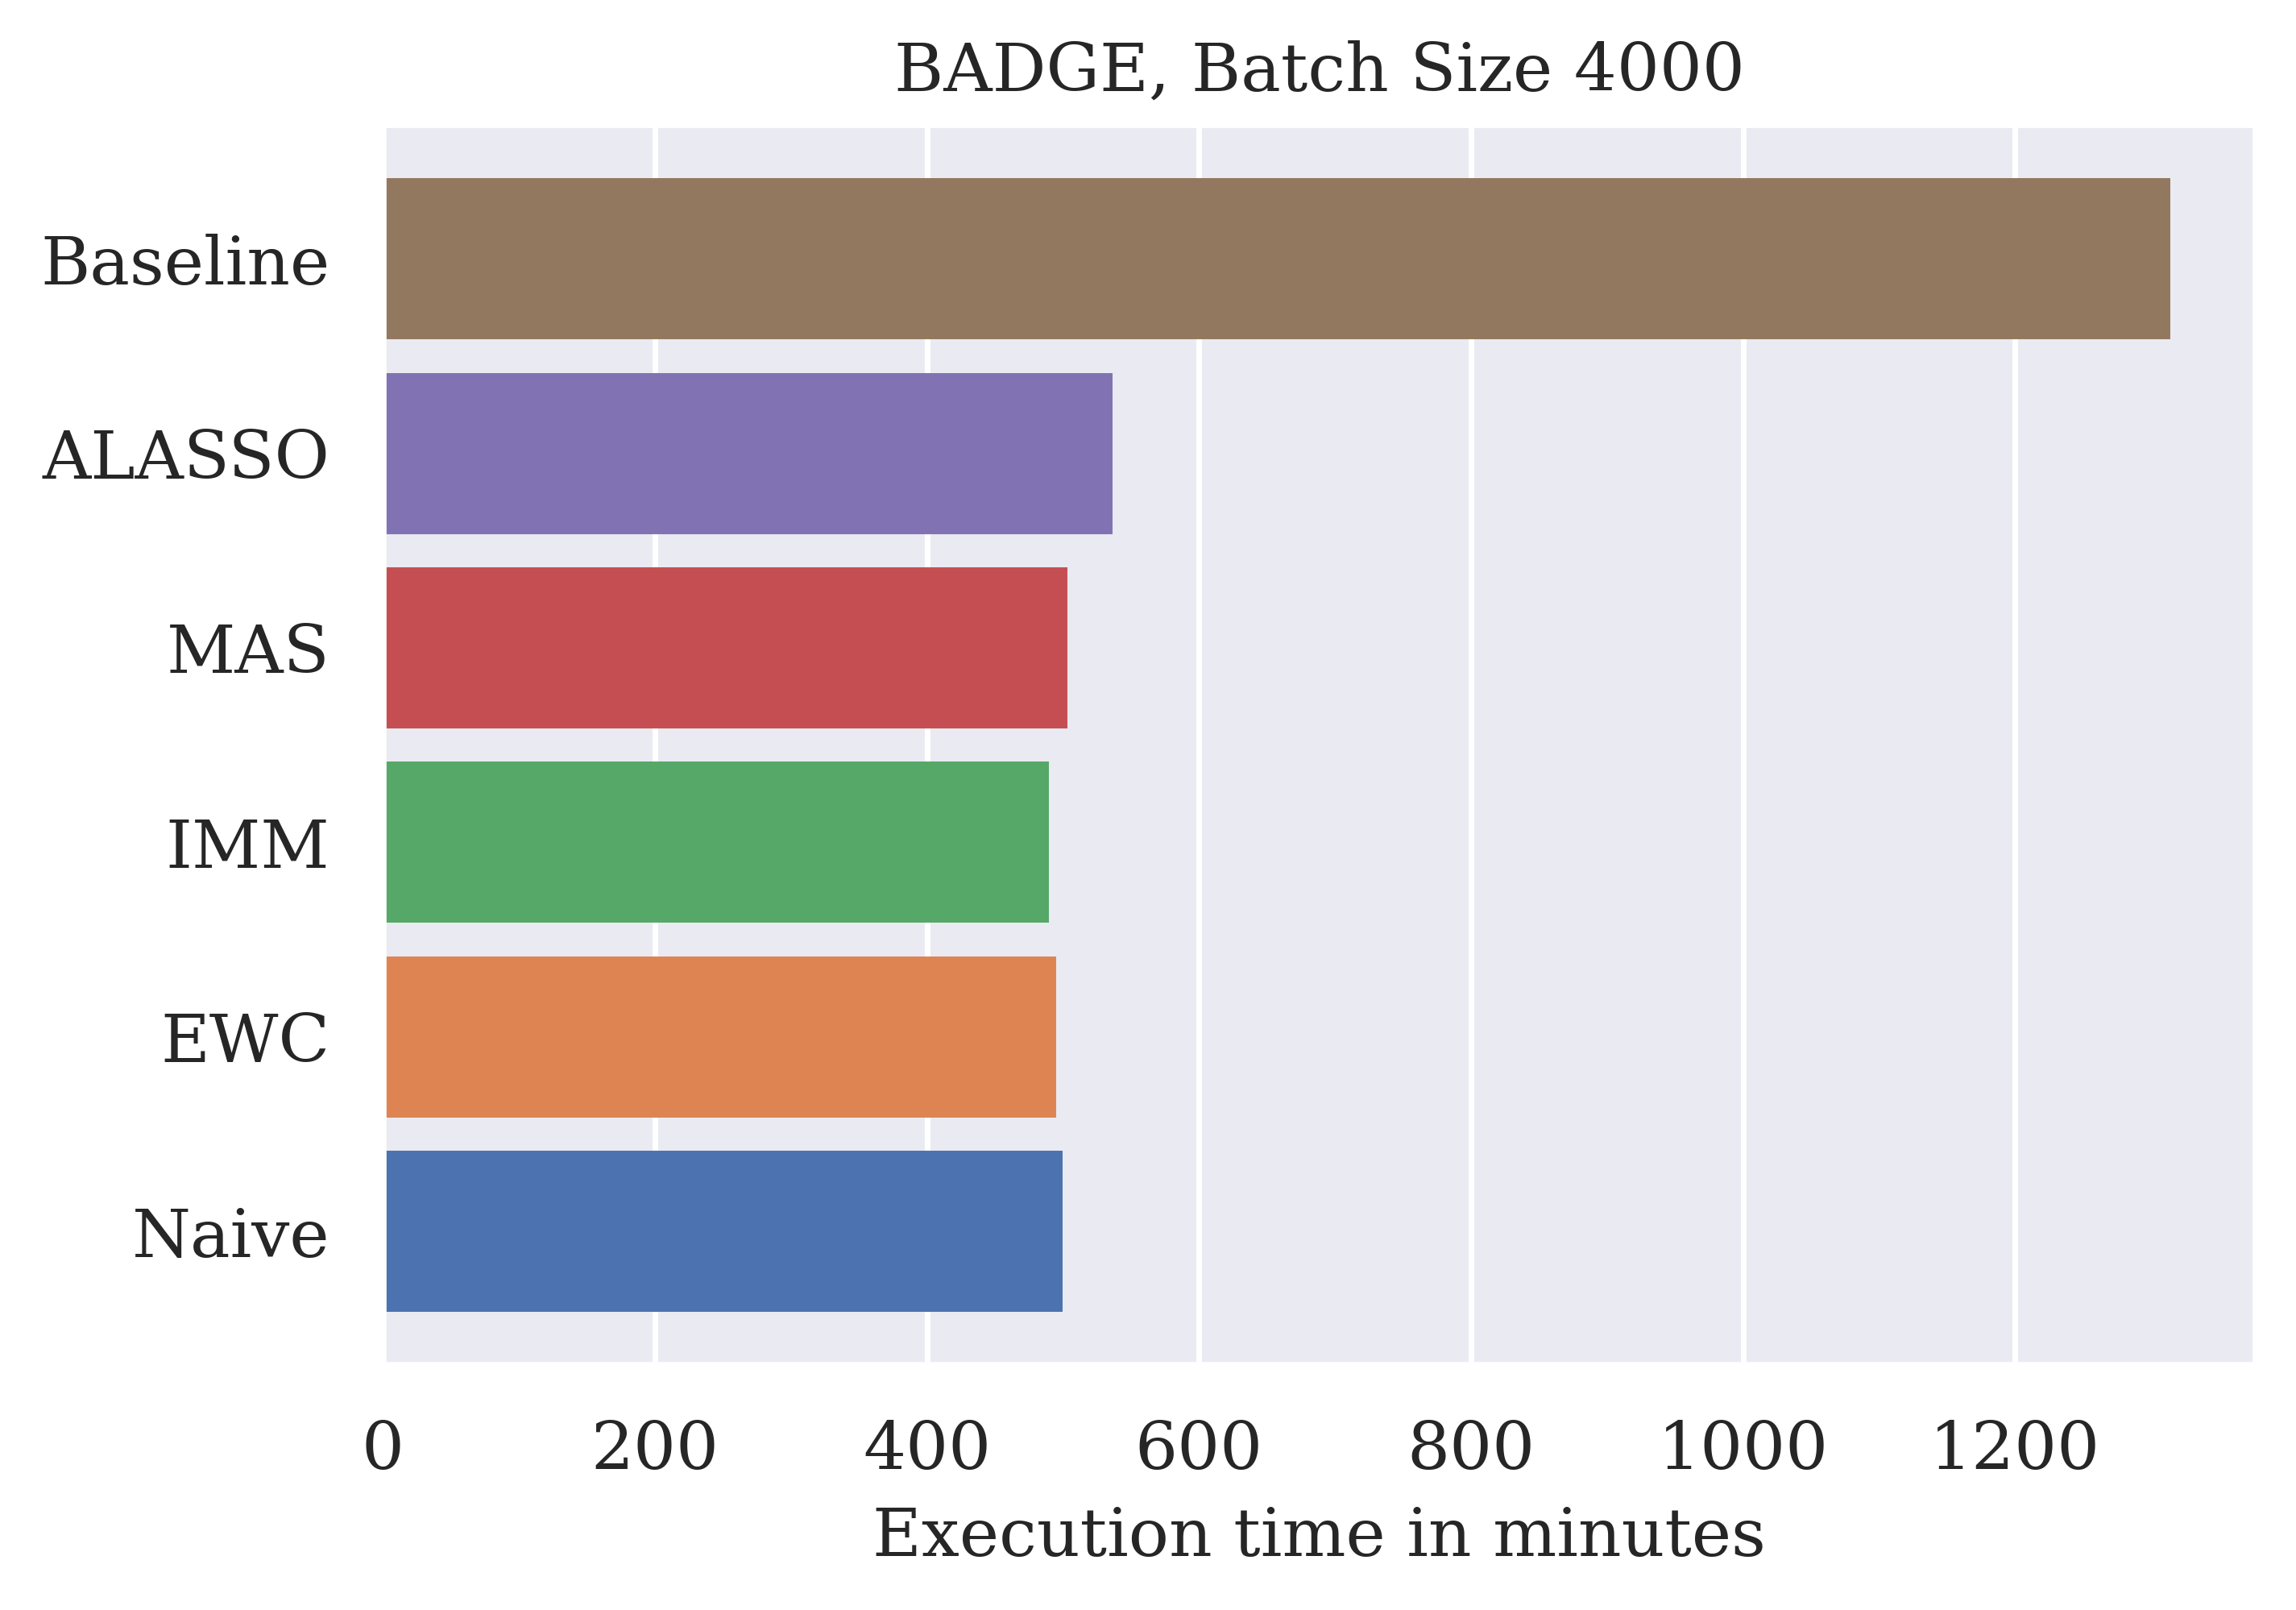
\includegraphics[width=0.32\linewidth]{images/results_CAL/badge_4000b_time.png} \hfill
%     \caption{Comparison of execution time of regularization-based continual learning strategies
%     with batch size 4000.}
%     \label{fig:Evaluation:Results:CAL:4000bTime}
% \end{figure}

%TODO: Decide whether to use table or barplots
\begin{table}[h]
    \centering
    \begin{tabular}{c | c c c c c } 
         & Random & \gls{lc} & \gls{bald} & CoreSet & \gls{badge}\\ 
        \hline
        Naive & 82 & 77 & 78 & 160 & 497 \\
        \gls{ewc} & 82 & 83 & 82 & 145 & 493\\
        \gls{imm} & 76 & 78 & 76 & 129 & 487\\
        \gls{mas} & 81 & 88 & 81 & 145 & 501\\
        \gls{alasso} & 118 & 127 & 120 & 189 & 534\\
        \hline 
        Baseline & 717 & 712 & 721 & 782 & 1311 \\
    \end{tabular}
    \caption{Comparison of execution time of regularization-based continual learning strategies
    with batch size 4000.}
    \label{fig:Evaluation:CAL:4000bTime}
\end{table}



\subsubsection{Influence of Batch Size}
\label{sec:Evaluation:Results:CAL:BatchSize}

\begin{figure}[h]
    \centering
    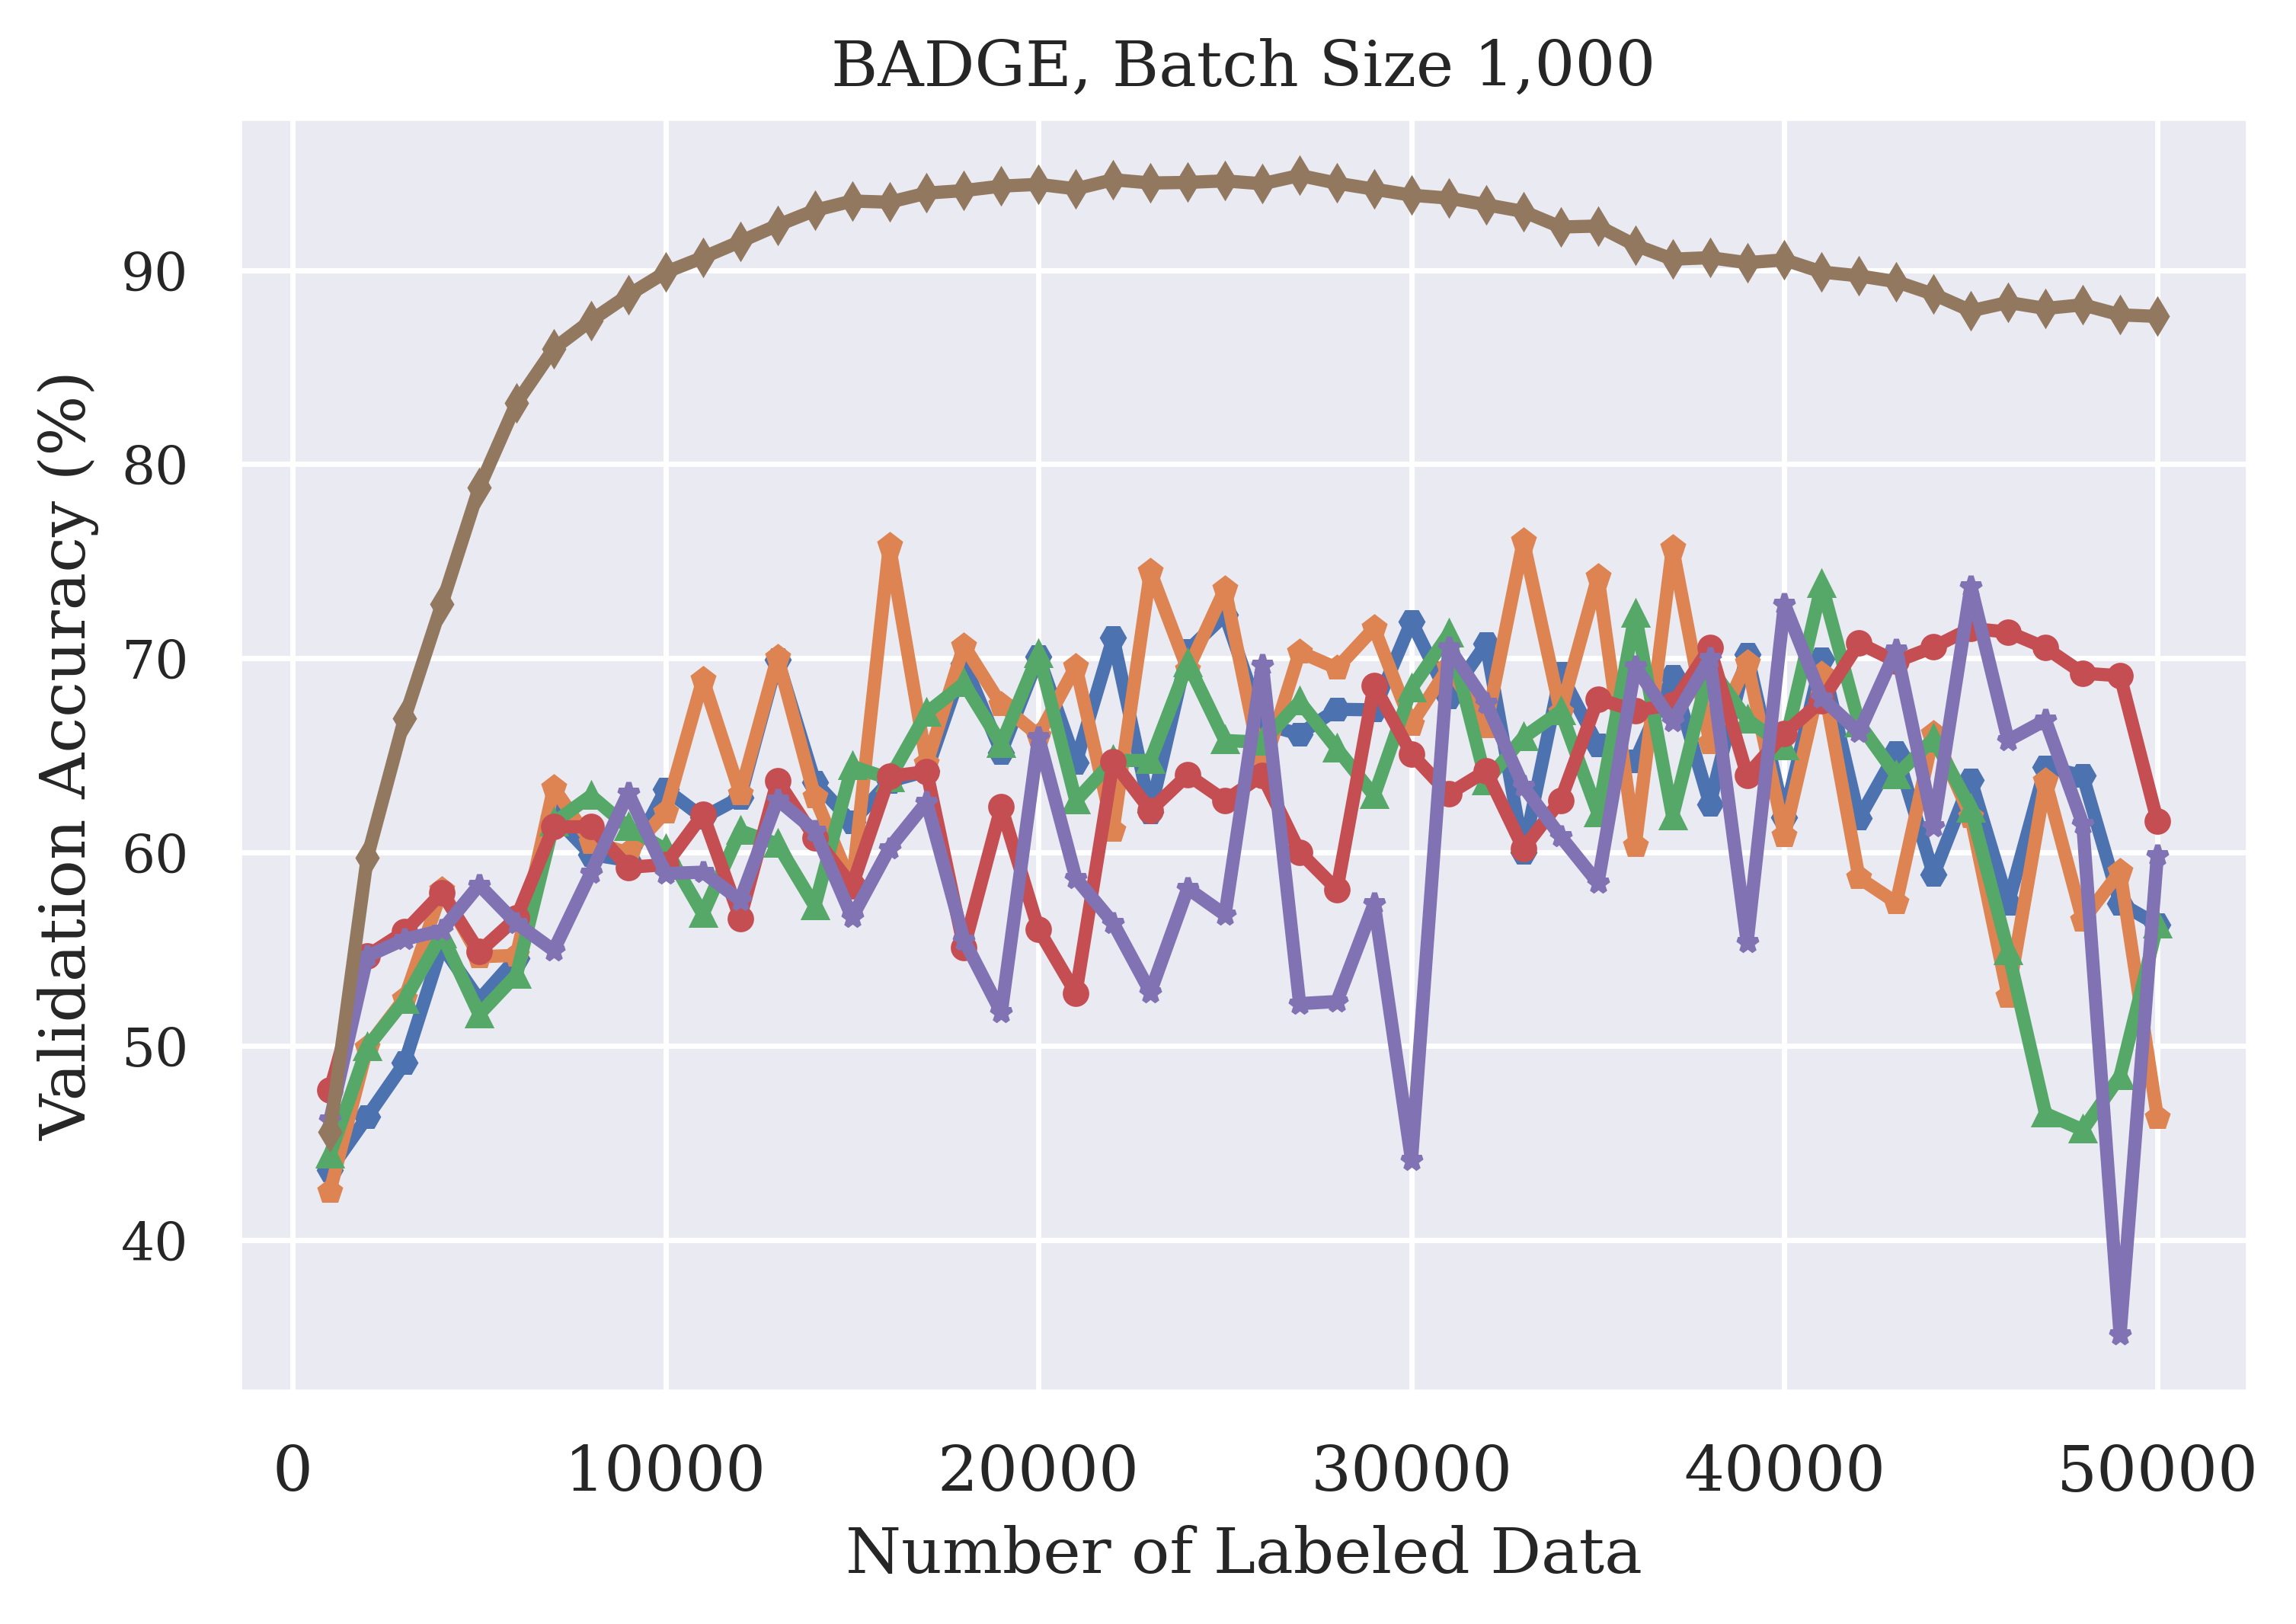
\includegraphics[width=0.32\linewidth]{images/results_CAL/badge_1000b_acc.png} \hfill
    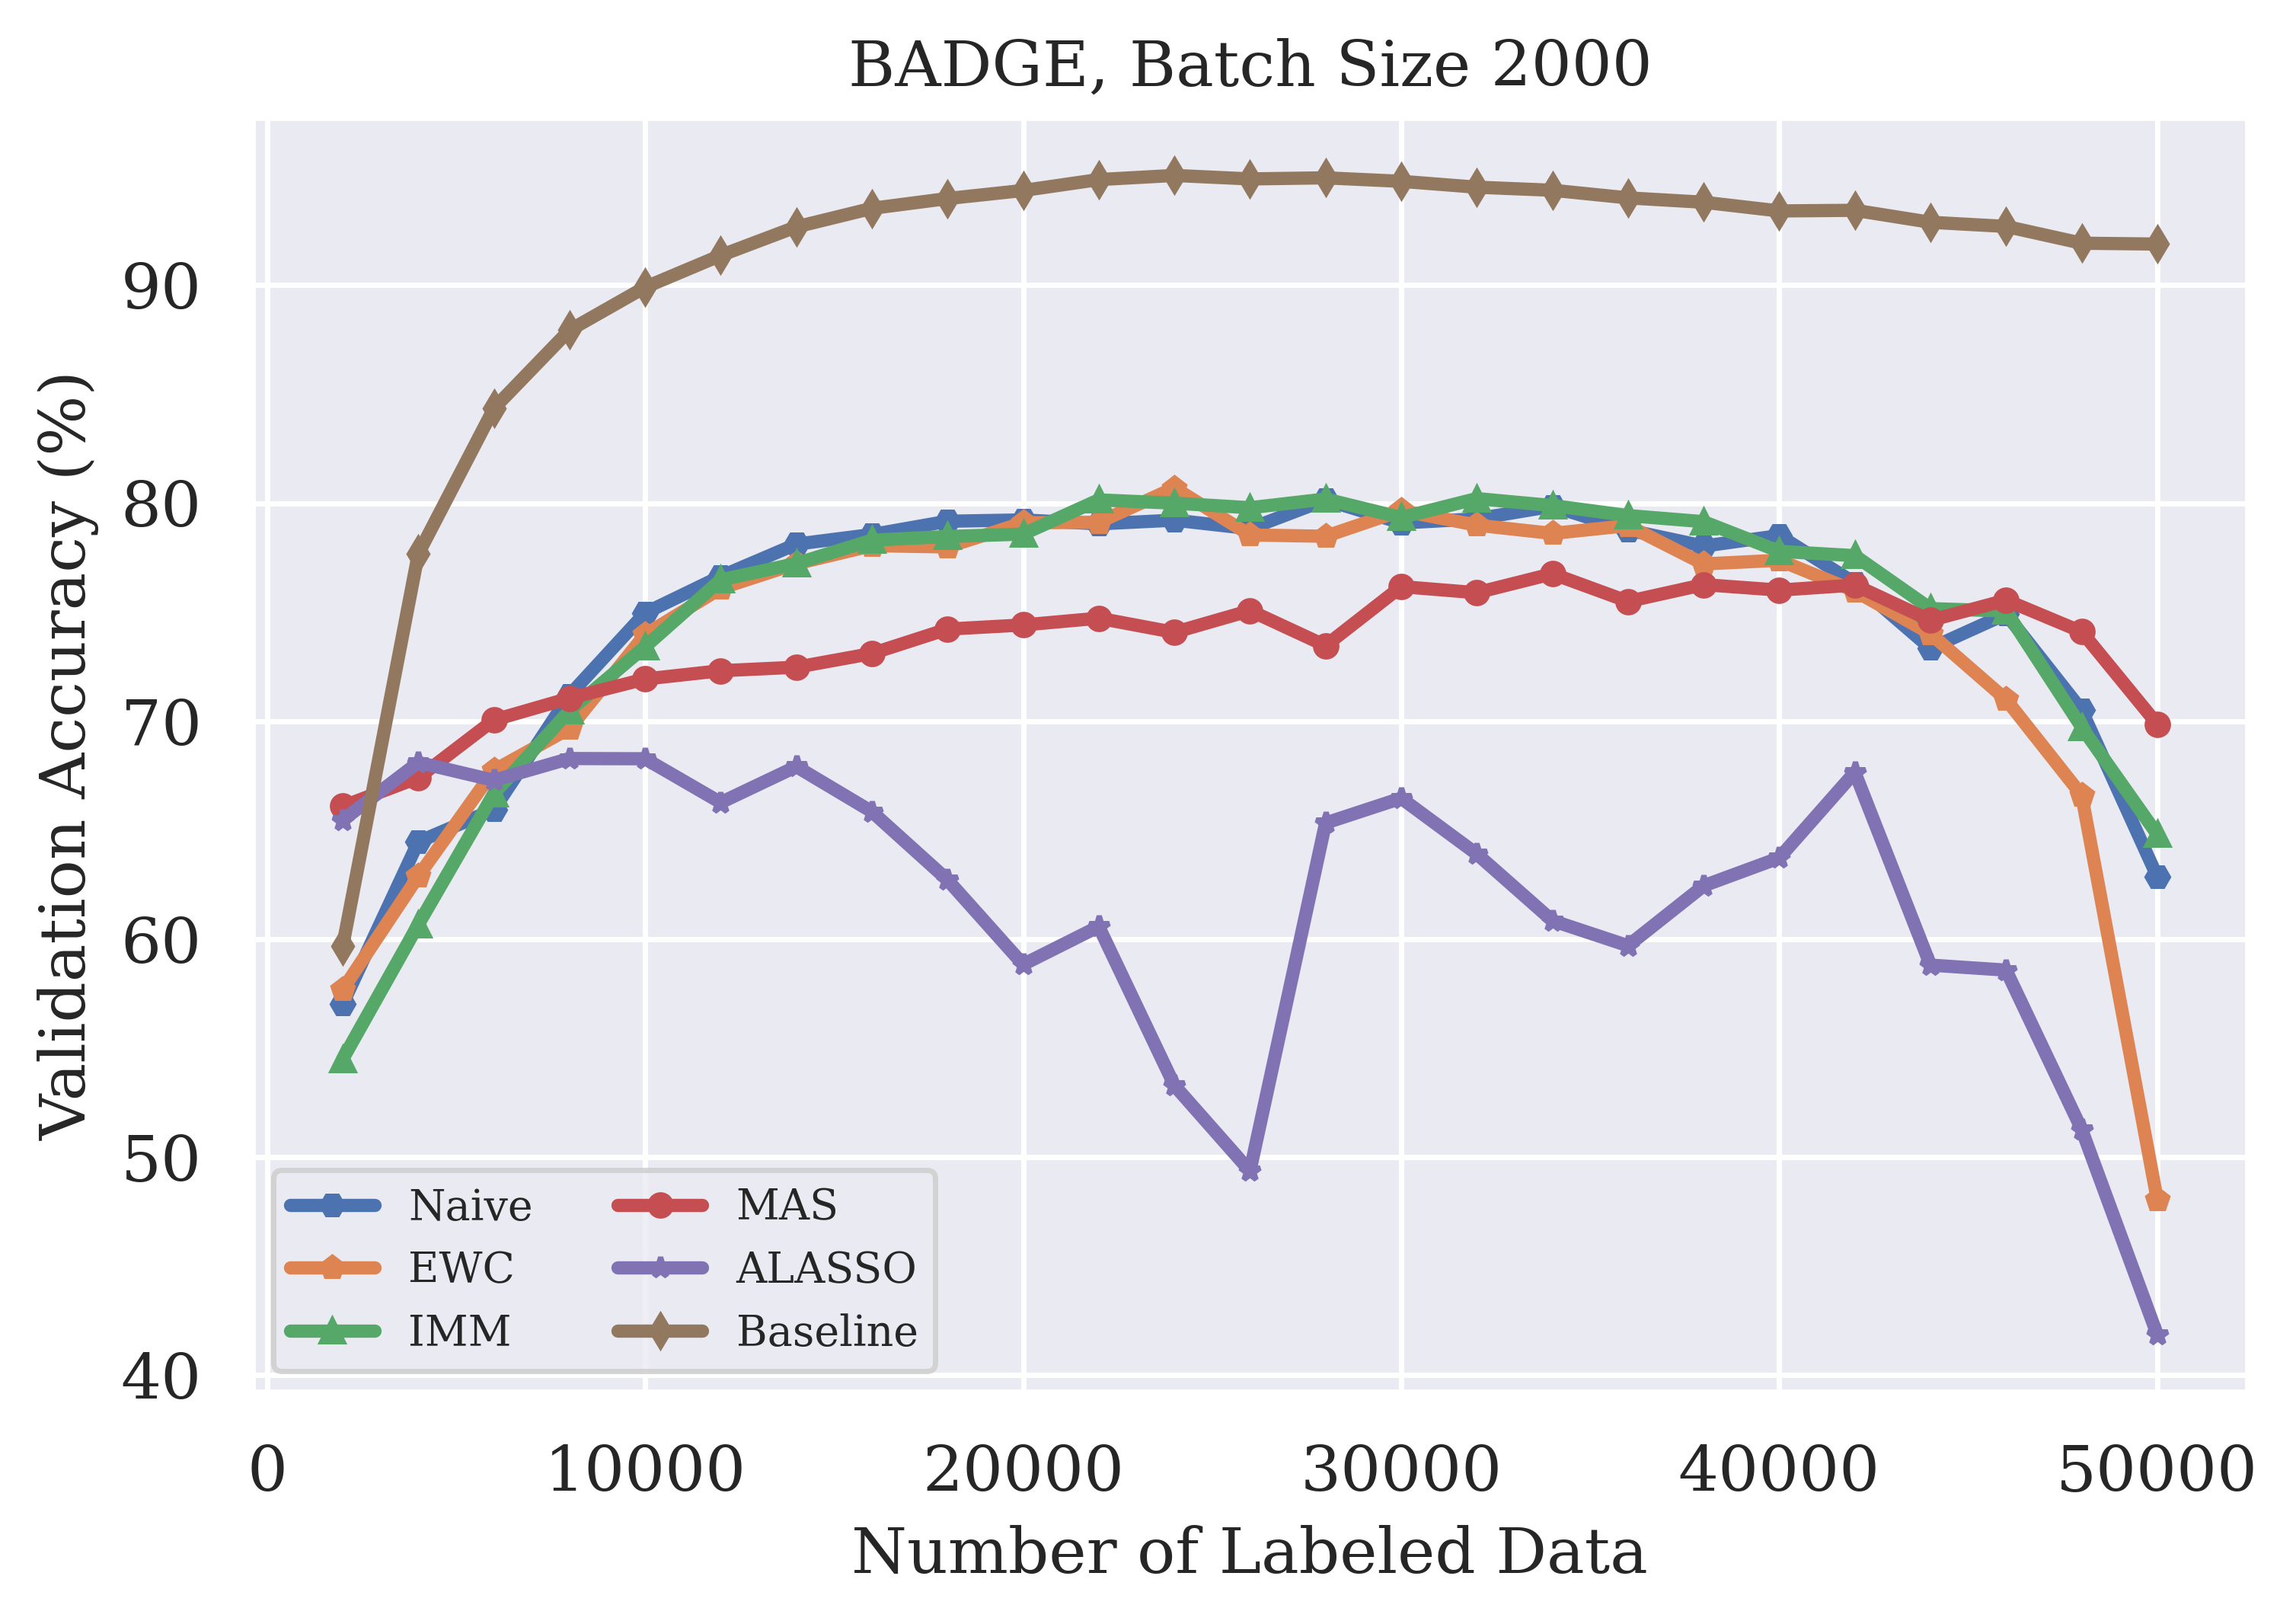
\includegraphics[width=0.32\linewidth]{images/results_CAL/badge_2000b_acc.png} \hfill
    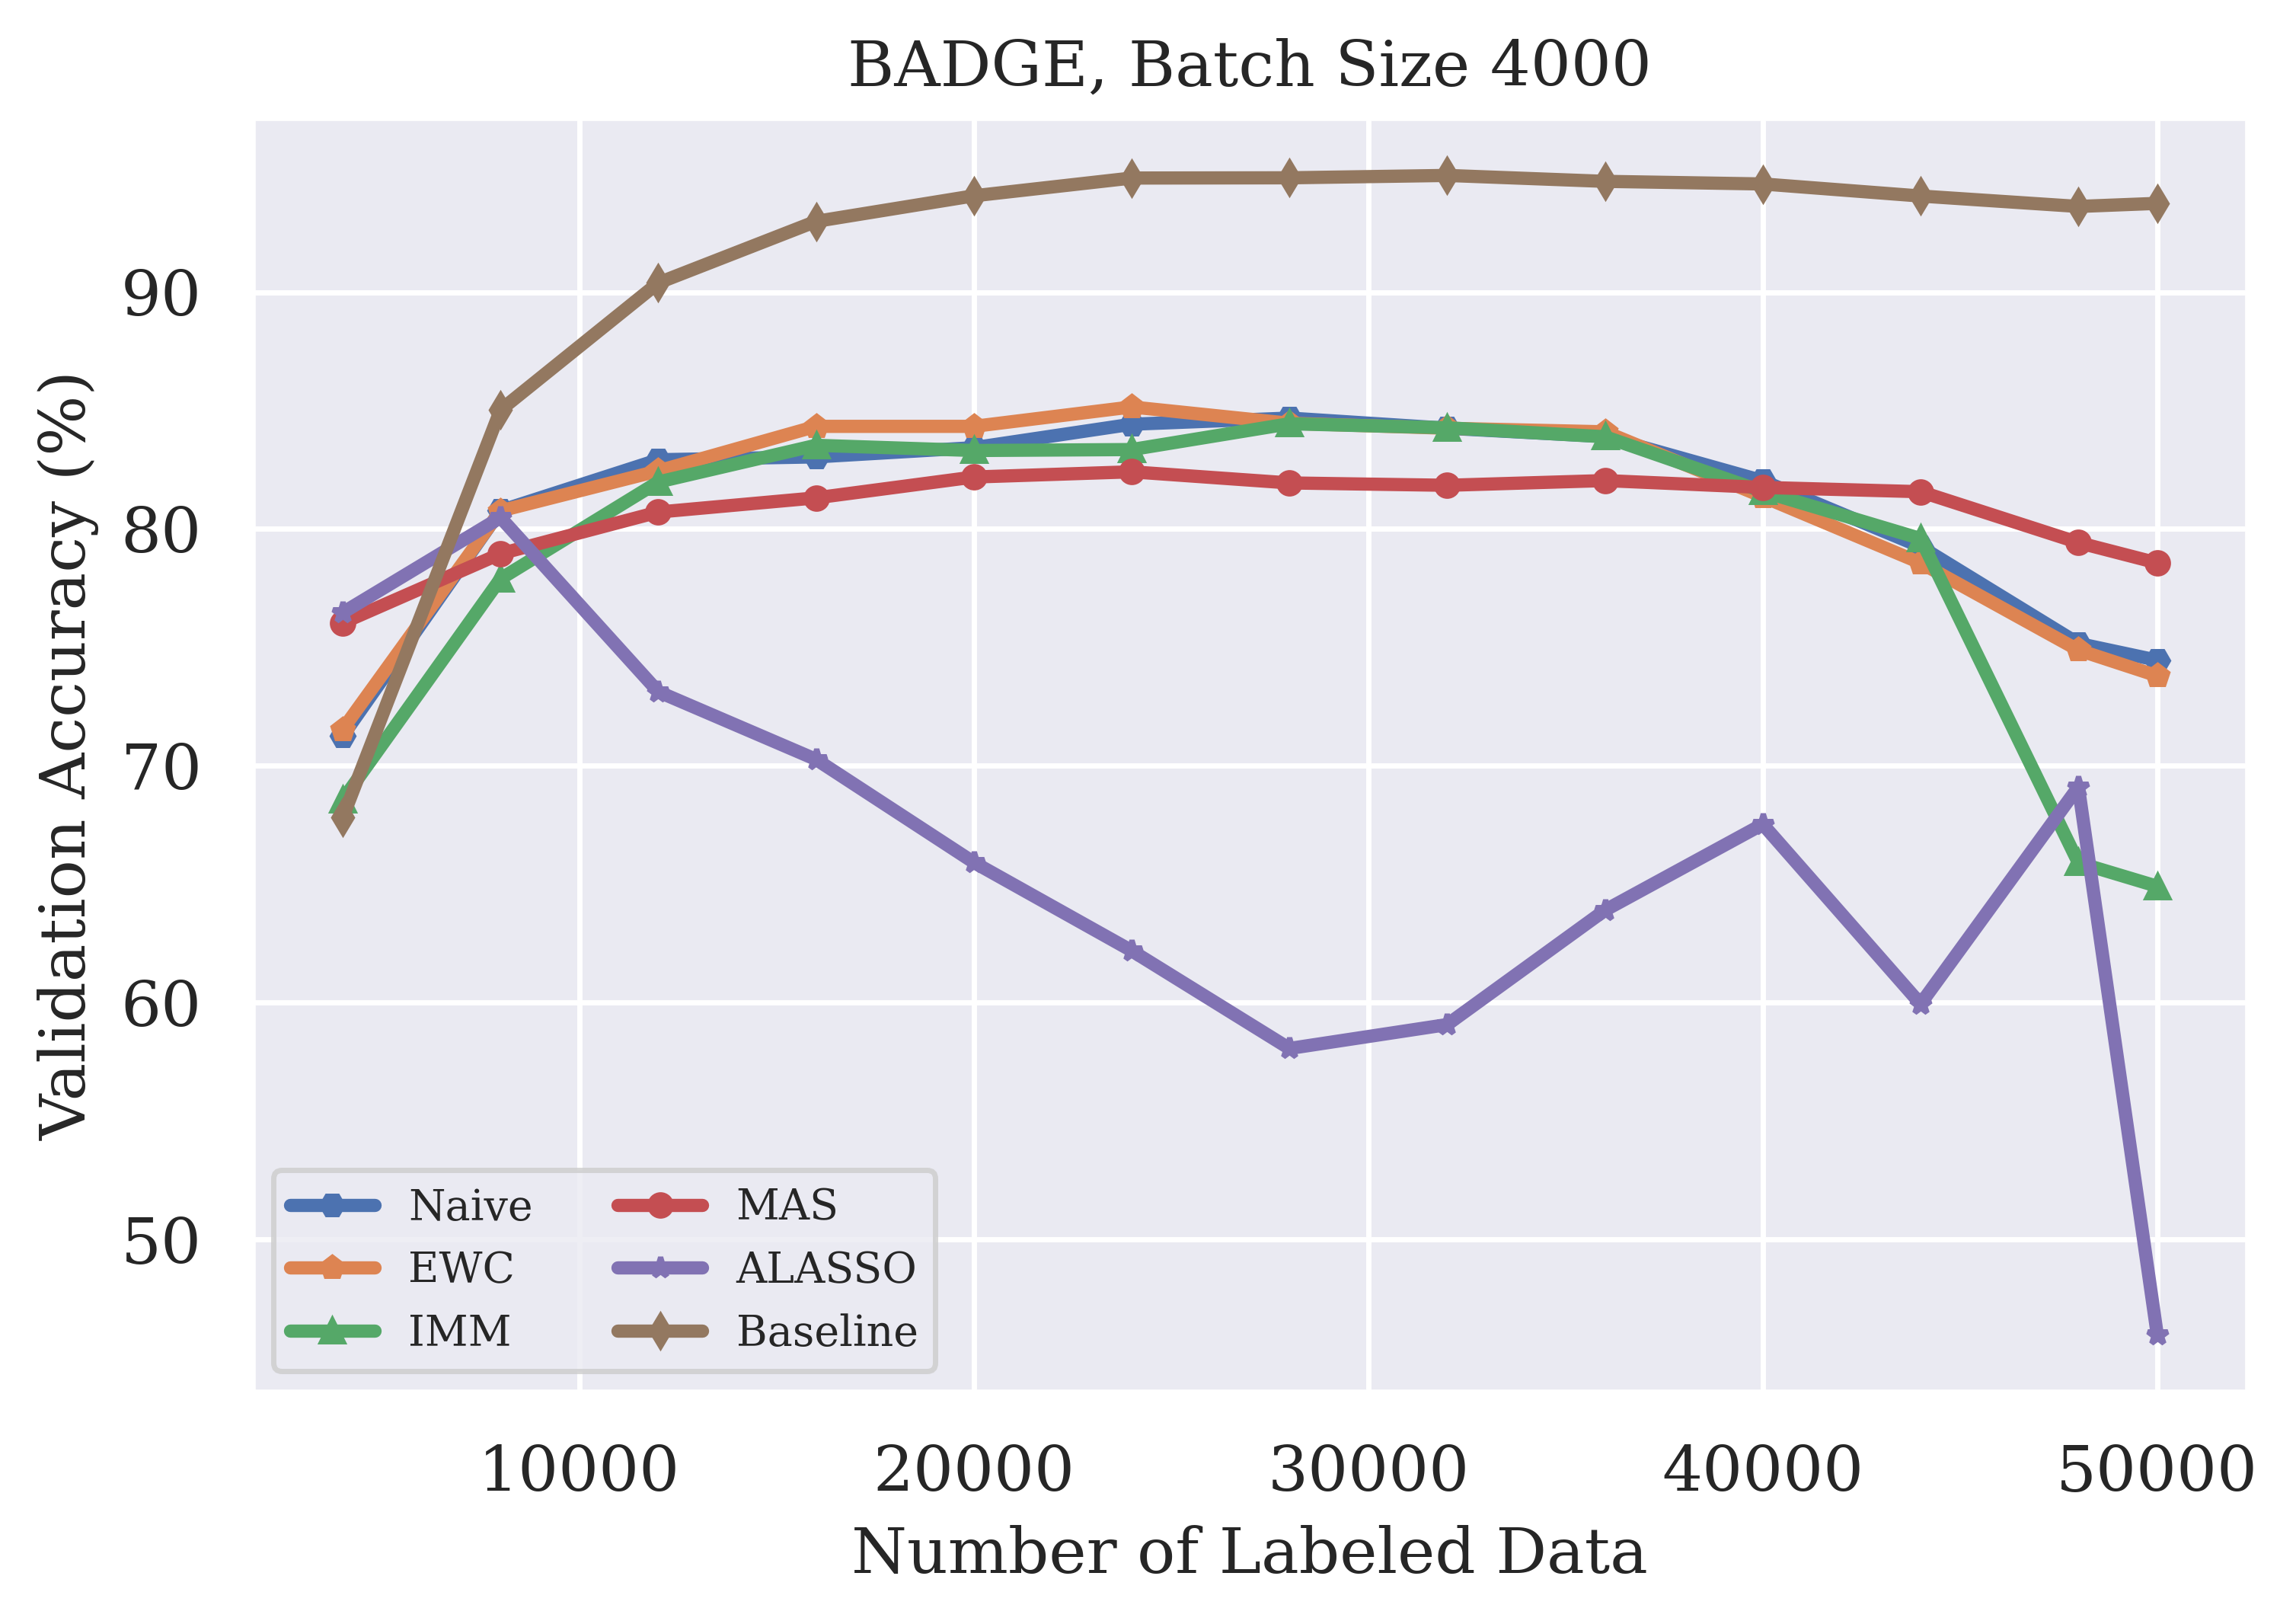
\includegraphics[width=0.32\linewidth]{images/results_CAL/badge_4000b_acc.png}
    \caption[Continual Active Learning with \gls{badge} with varying batch size]{Comparison of validation accuracy of Continual Learning strategies used with the Active Learning strategy
    \gls{badge}.}
    \label{fig:Evaluation:Results:CAL:VaryBatchSizeAcc}
\end{figure}

% \begin{figure}[h]
%     \centering
%     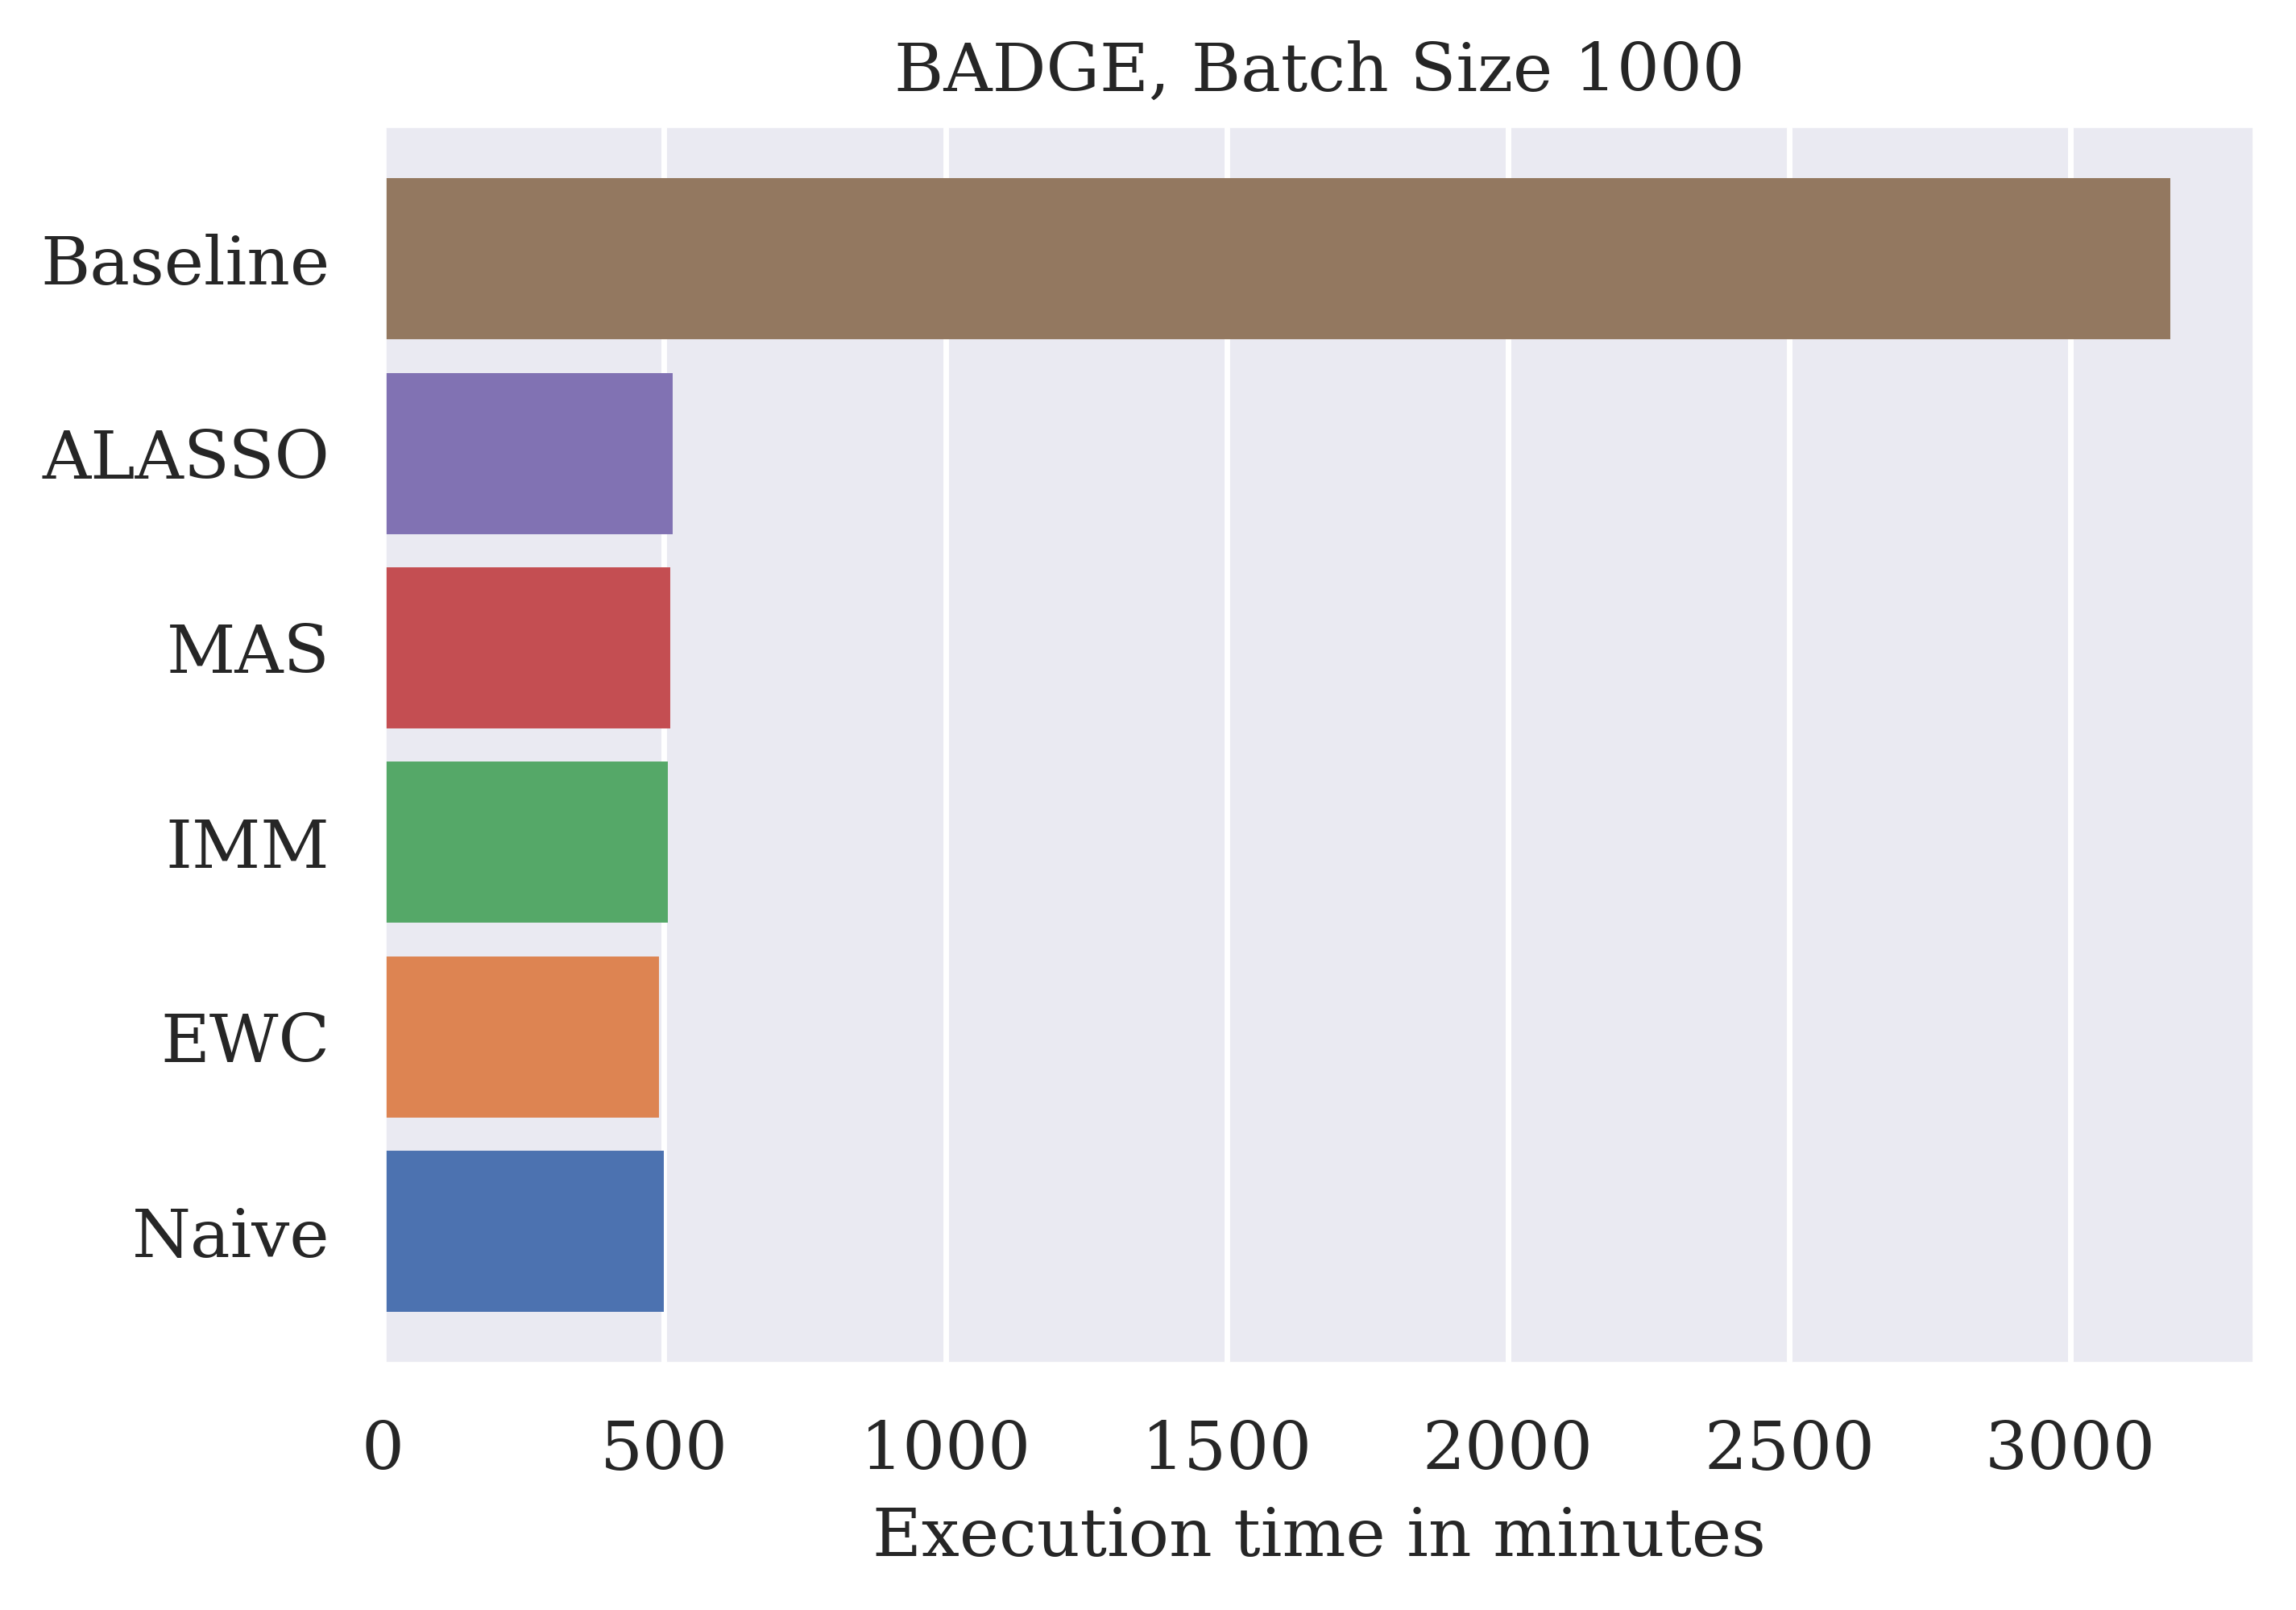
\includegraphics[width=0.32\linewidth]{images/results_CAL/badge_1000b_time.png} \hfill
%     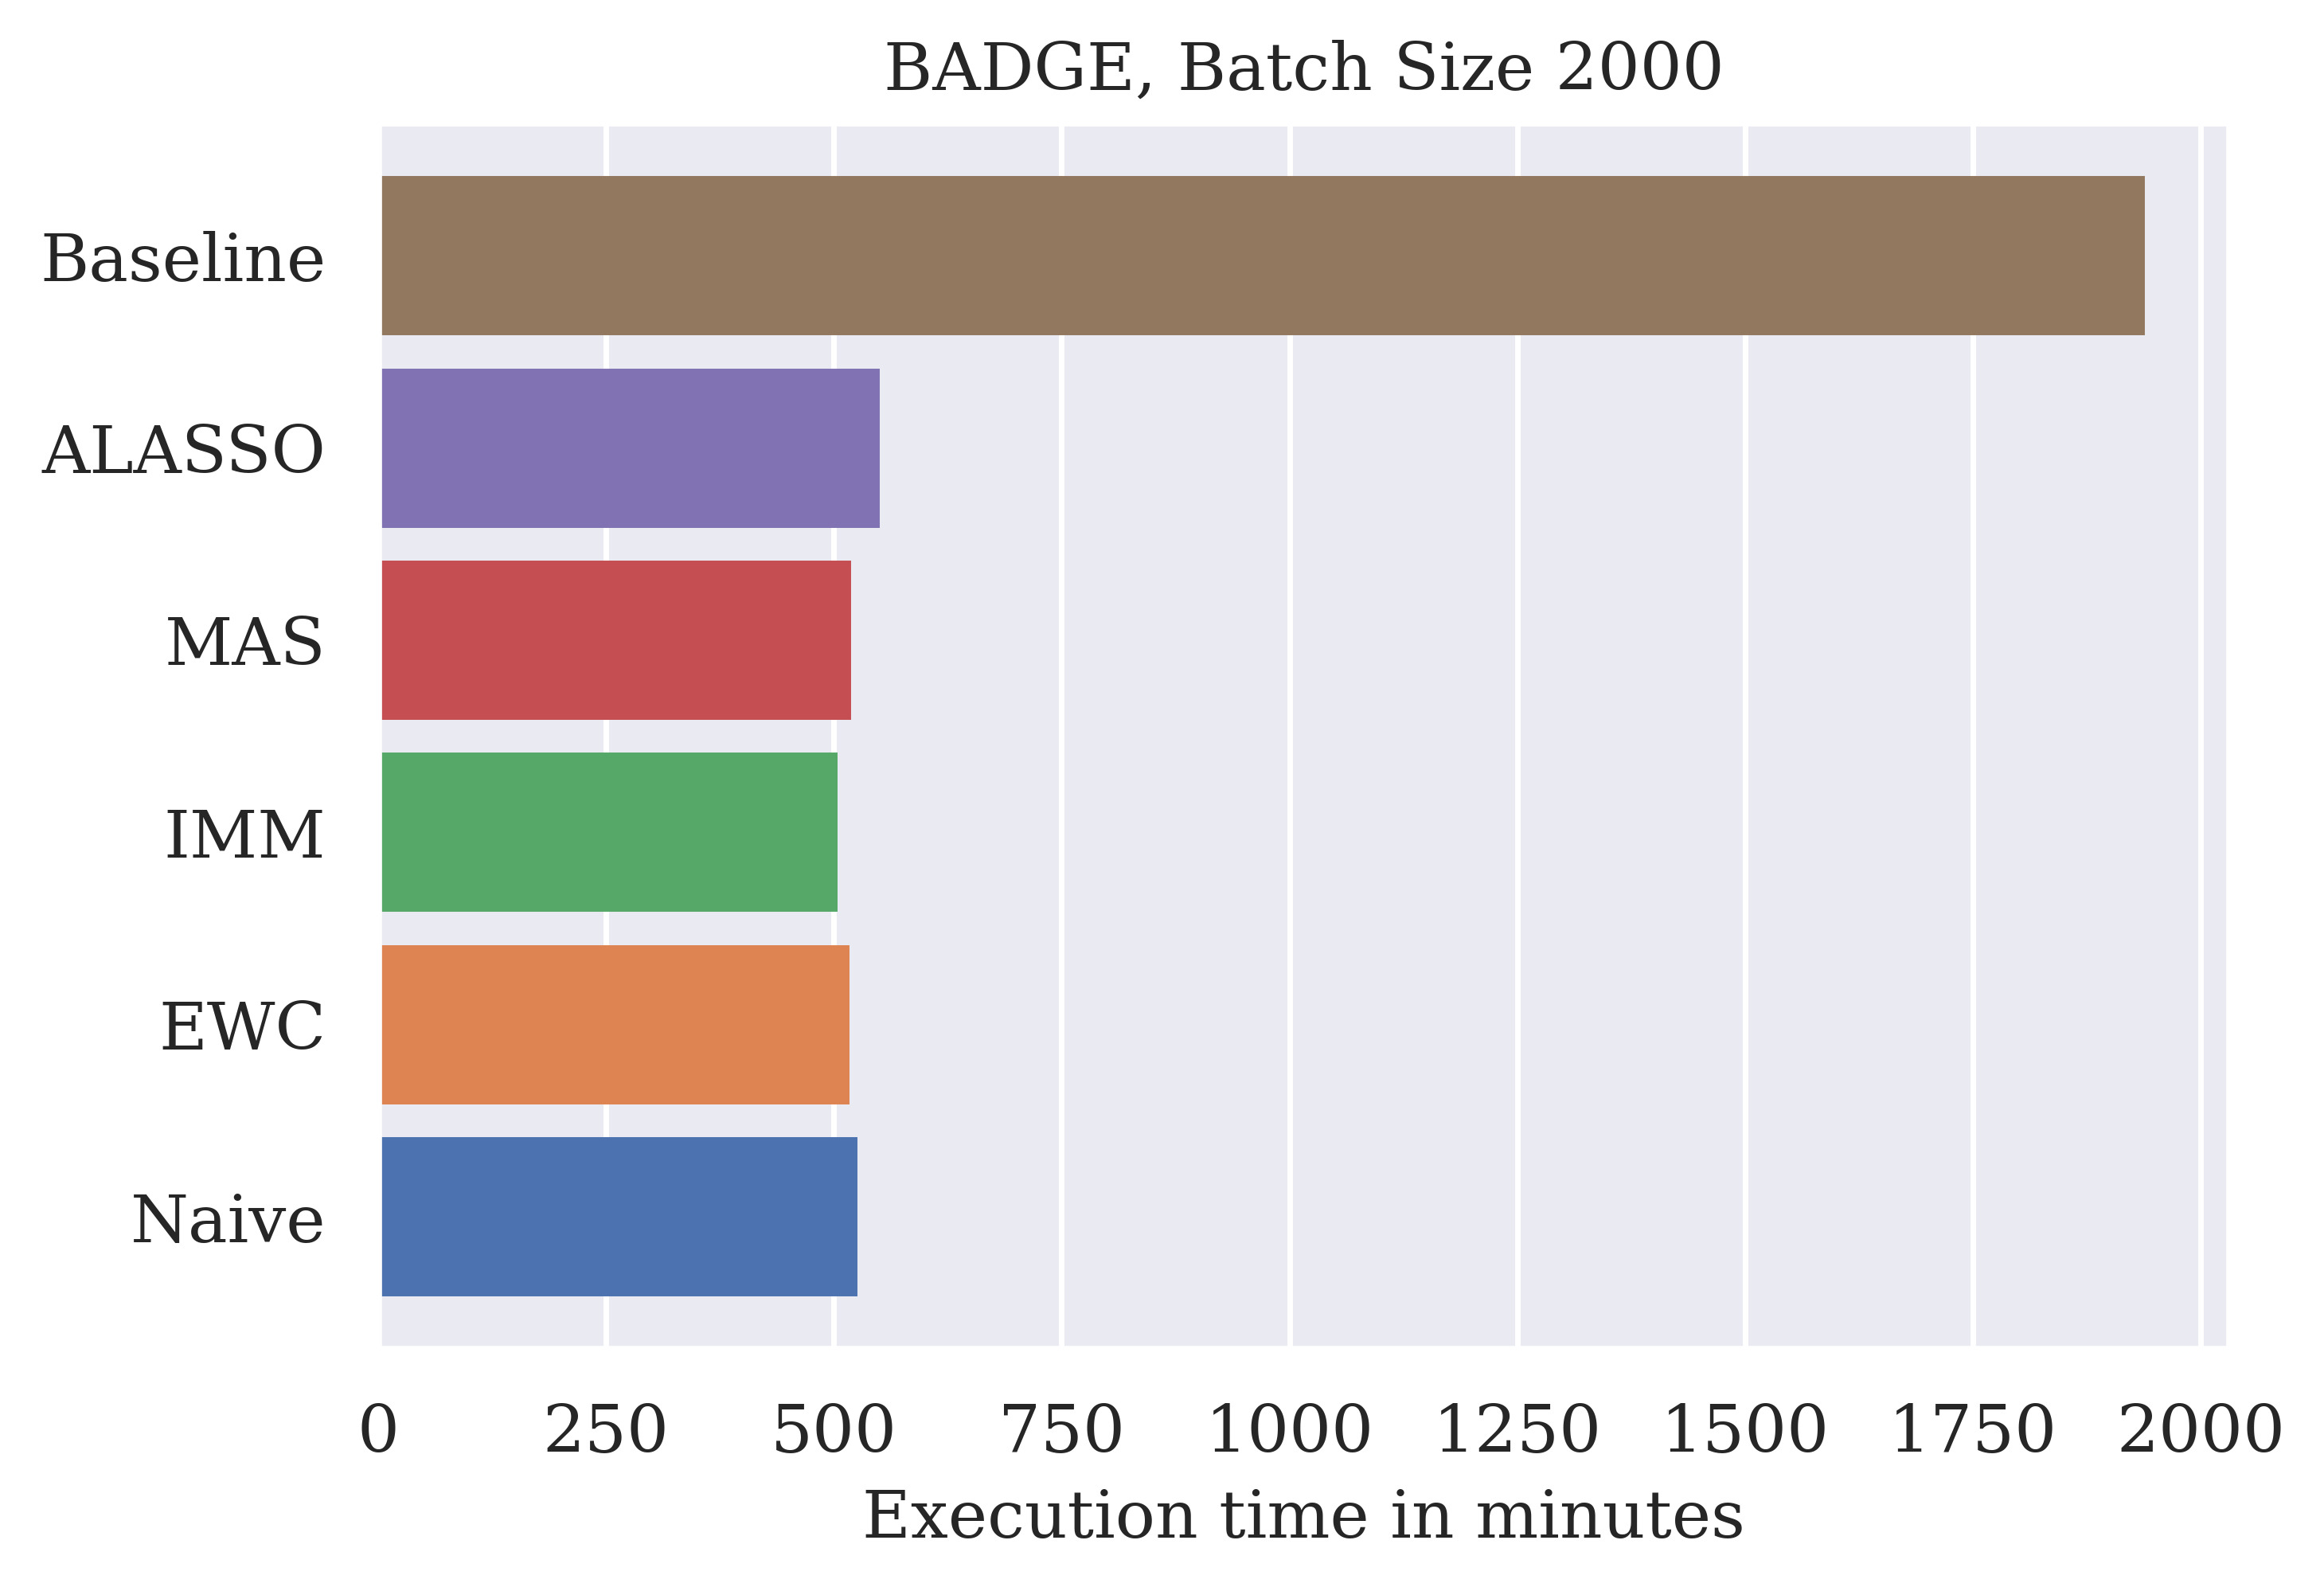
\includegraphics[width=0.32\linewidth]{images/results_CAL/badge_2000b_time.png} \hfill
%     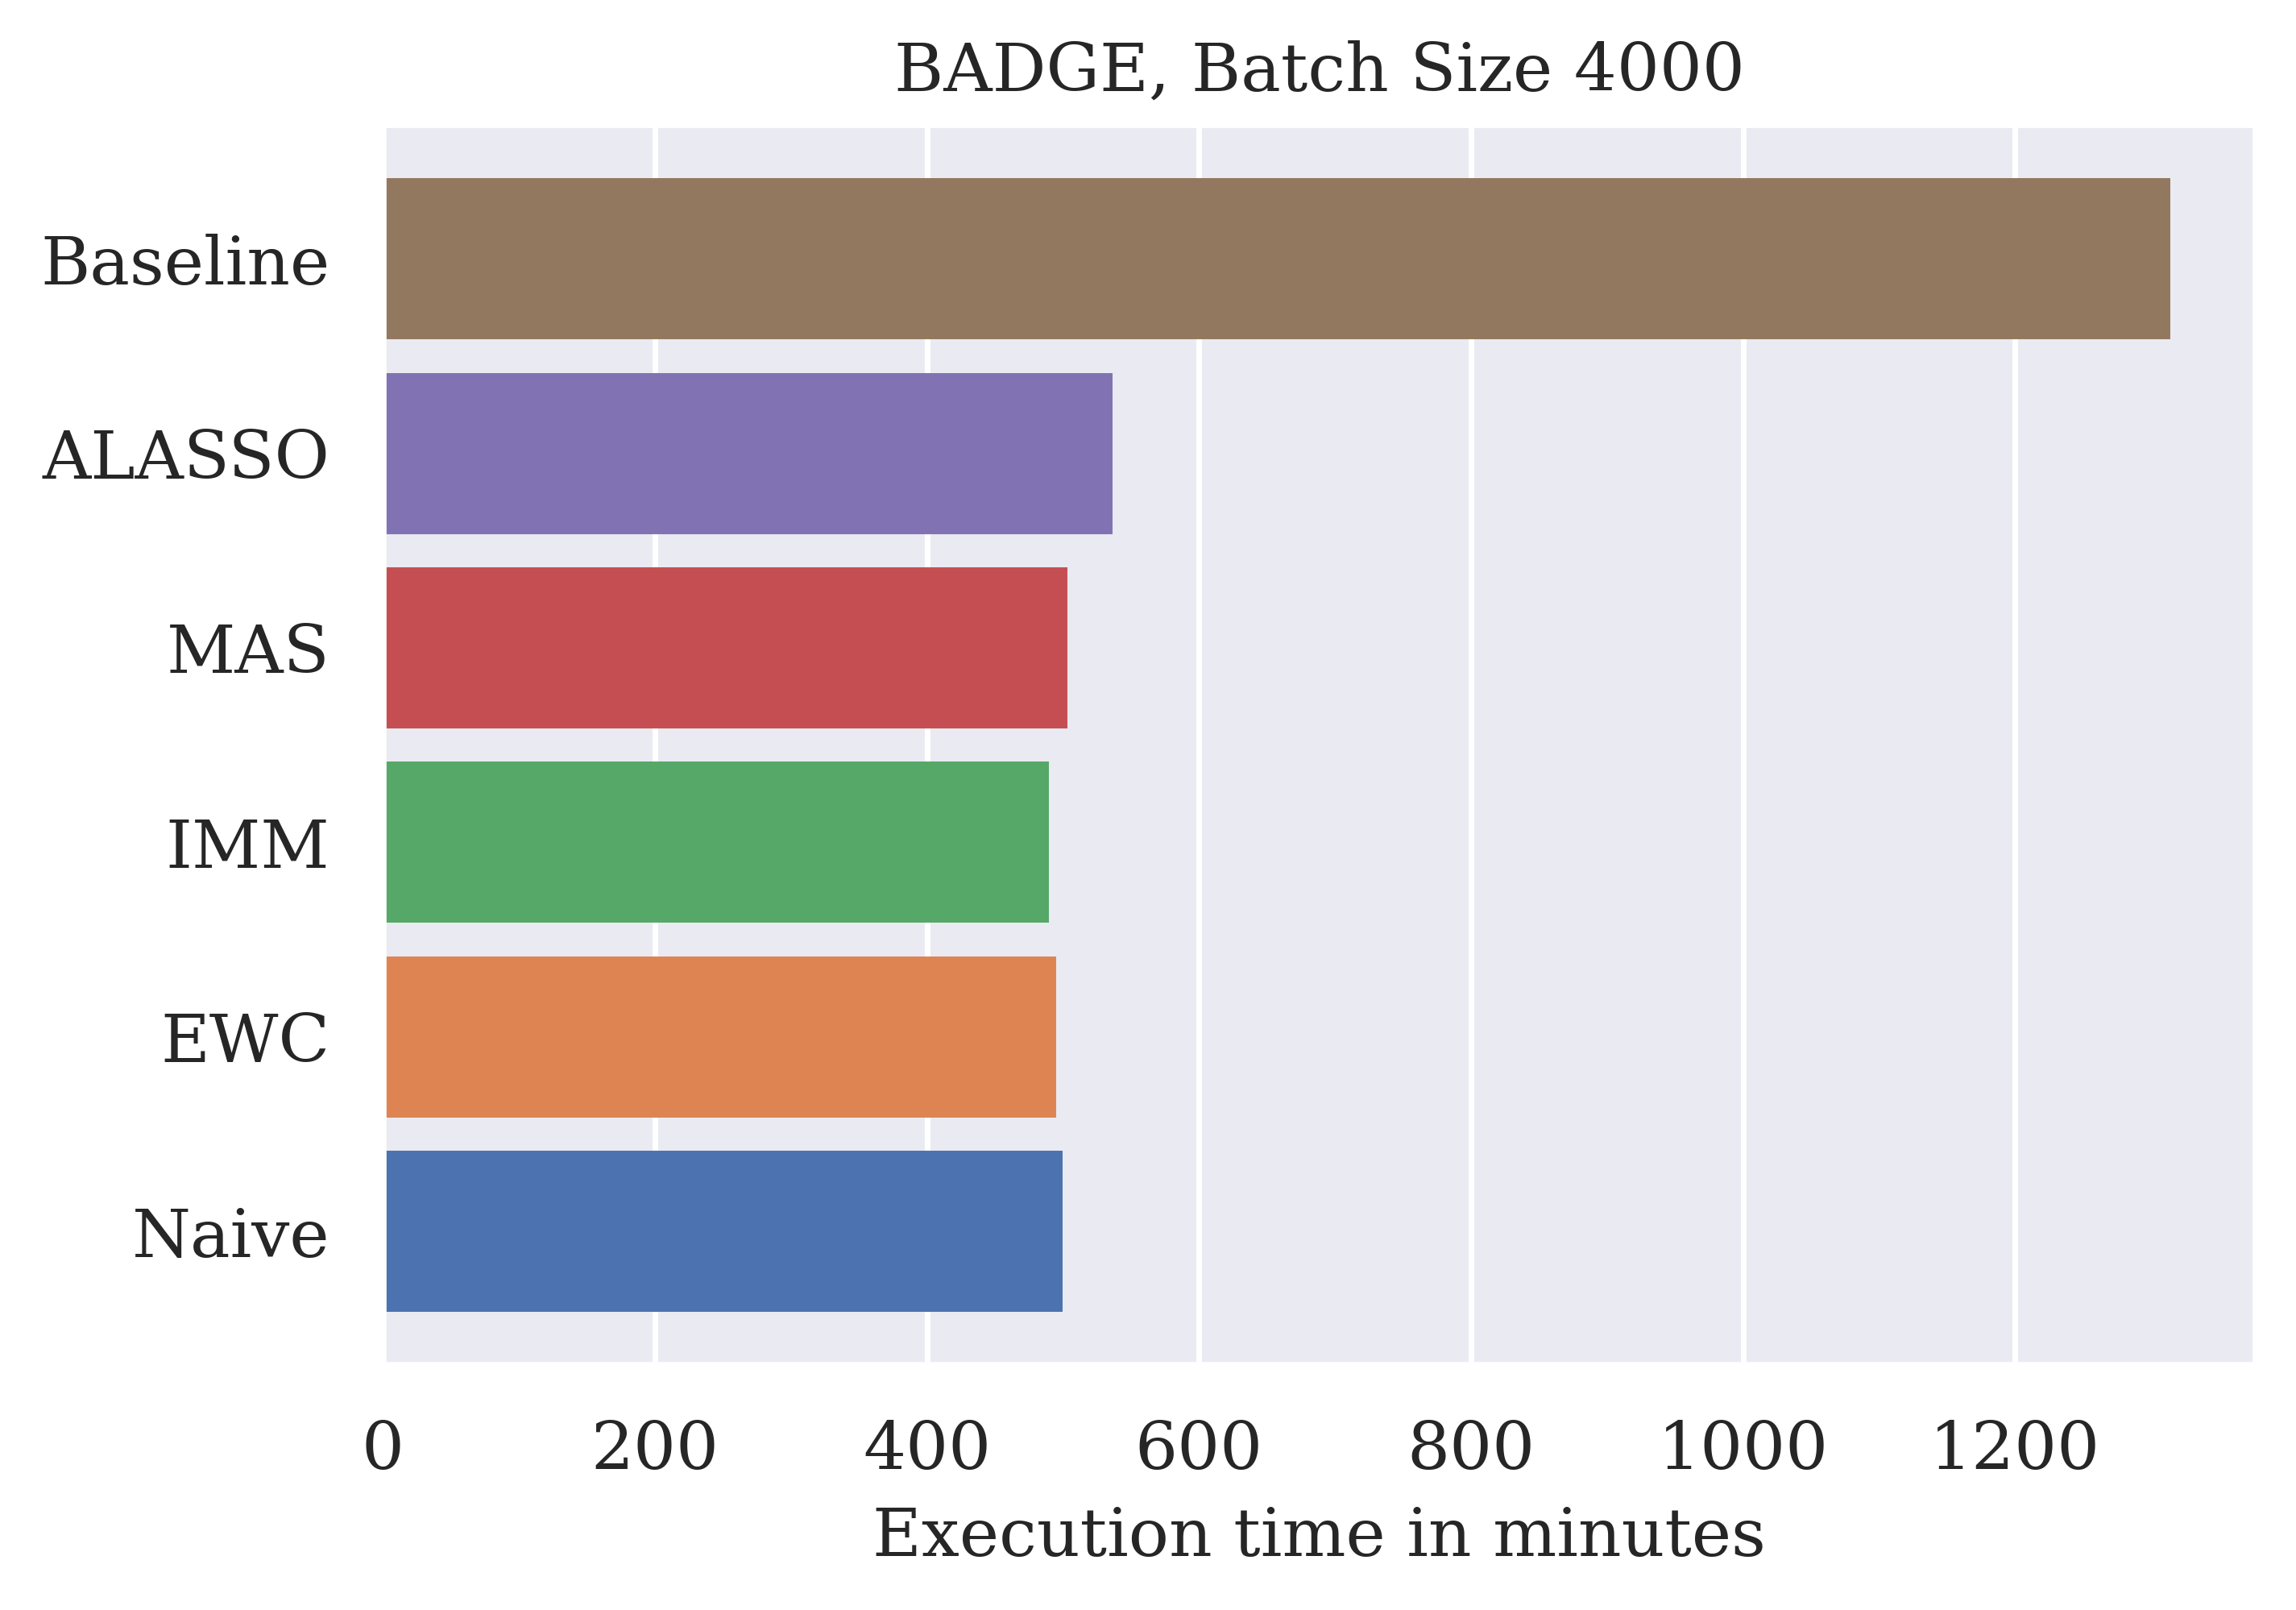
\includegraphics[width=0.32\linewidth]{images/results_CAL/badge_4000b_time.png}
%     \caption[Continual Active Learning with \gls{badge} with varying batch size]{Comparison of validation accuracy of Continual Learning strategies used with the Active Learning strategy
%     \gls{badge}.}
%     \label{fig:Evaluation:Results:CAL:VaryBatchSizeTime}
% \end{figure}

\begin{table}[h]
    \centering
    \begin{tabular}{c | c c c c c c} 
        Batch Size & Baseline & Naive & \gls{ewc} & \gls{imm} & \gls{mas} & \gls{alasso}\\ 
        \hline 
        4000 & 1311 & 497 & 493 & 487 & 501 & 534 \\
        2000 & 1935 & 523 & 513 & 500 & 515 & 547 \\
        1000 & 3171 & 493 & 486 & 501 & 505 & 509 \\
    \end{tabular}
    \caption{Comparison of execution time of regularization-based continual learning strategies
    combined with \gls{badge}.}
    \label{fig:Evaluation:CAL:BadgeVaryBatchSizeTime}
\end{table}


\subsubsection{Delaying the Start of Continual Learning}
\label{sec:Evaluation:Results:CAL:Hybrid}
After running the experiments in section \ref{sec:Evaluation:Results:CAL:ALCL}, we notice that all of them demonstrate a significant discrepancy in validation accuracy between Active Learning and Continual Active Learning. To further investigate this gap,
we investigate a hybrid approach where we run Active learning for the first $i$ iterations before switching to Continual Active Learning. With these experiments we hope to decrease the gap in validation accuracy to Active Learning. We vary $i$ between 0 and 6,
and perform two sets of experiments, one using the Continual Learning strategy \gls{mas} and the other using \gls{ewc}. In both experiments, we use the Active Learning strategy \gls{badge}. The results of the two sets of experiments can be found in figure 
\ref{fig:Evaluation:Results:CAL:DelayedStart}. For \gls{mas} and \gls{ewc}, the validation accuracy drops immediately after switching from Active Learning to Continual Active Learning. However, in the long run the \gls{mas} strategy retains the validation accuracy better than \gls{ewc}.
We also notice that while the validation accuracy does drop after switching to Continual Active Learning, it is higher at a fixed cycle than when switching to Continual Active Learning in an earlier cycle. \par

%TODO: Hier die Bilder noch ändern sodass sie nicht aus Powerpoint sind
\begin{figure}[h]
    \centering
    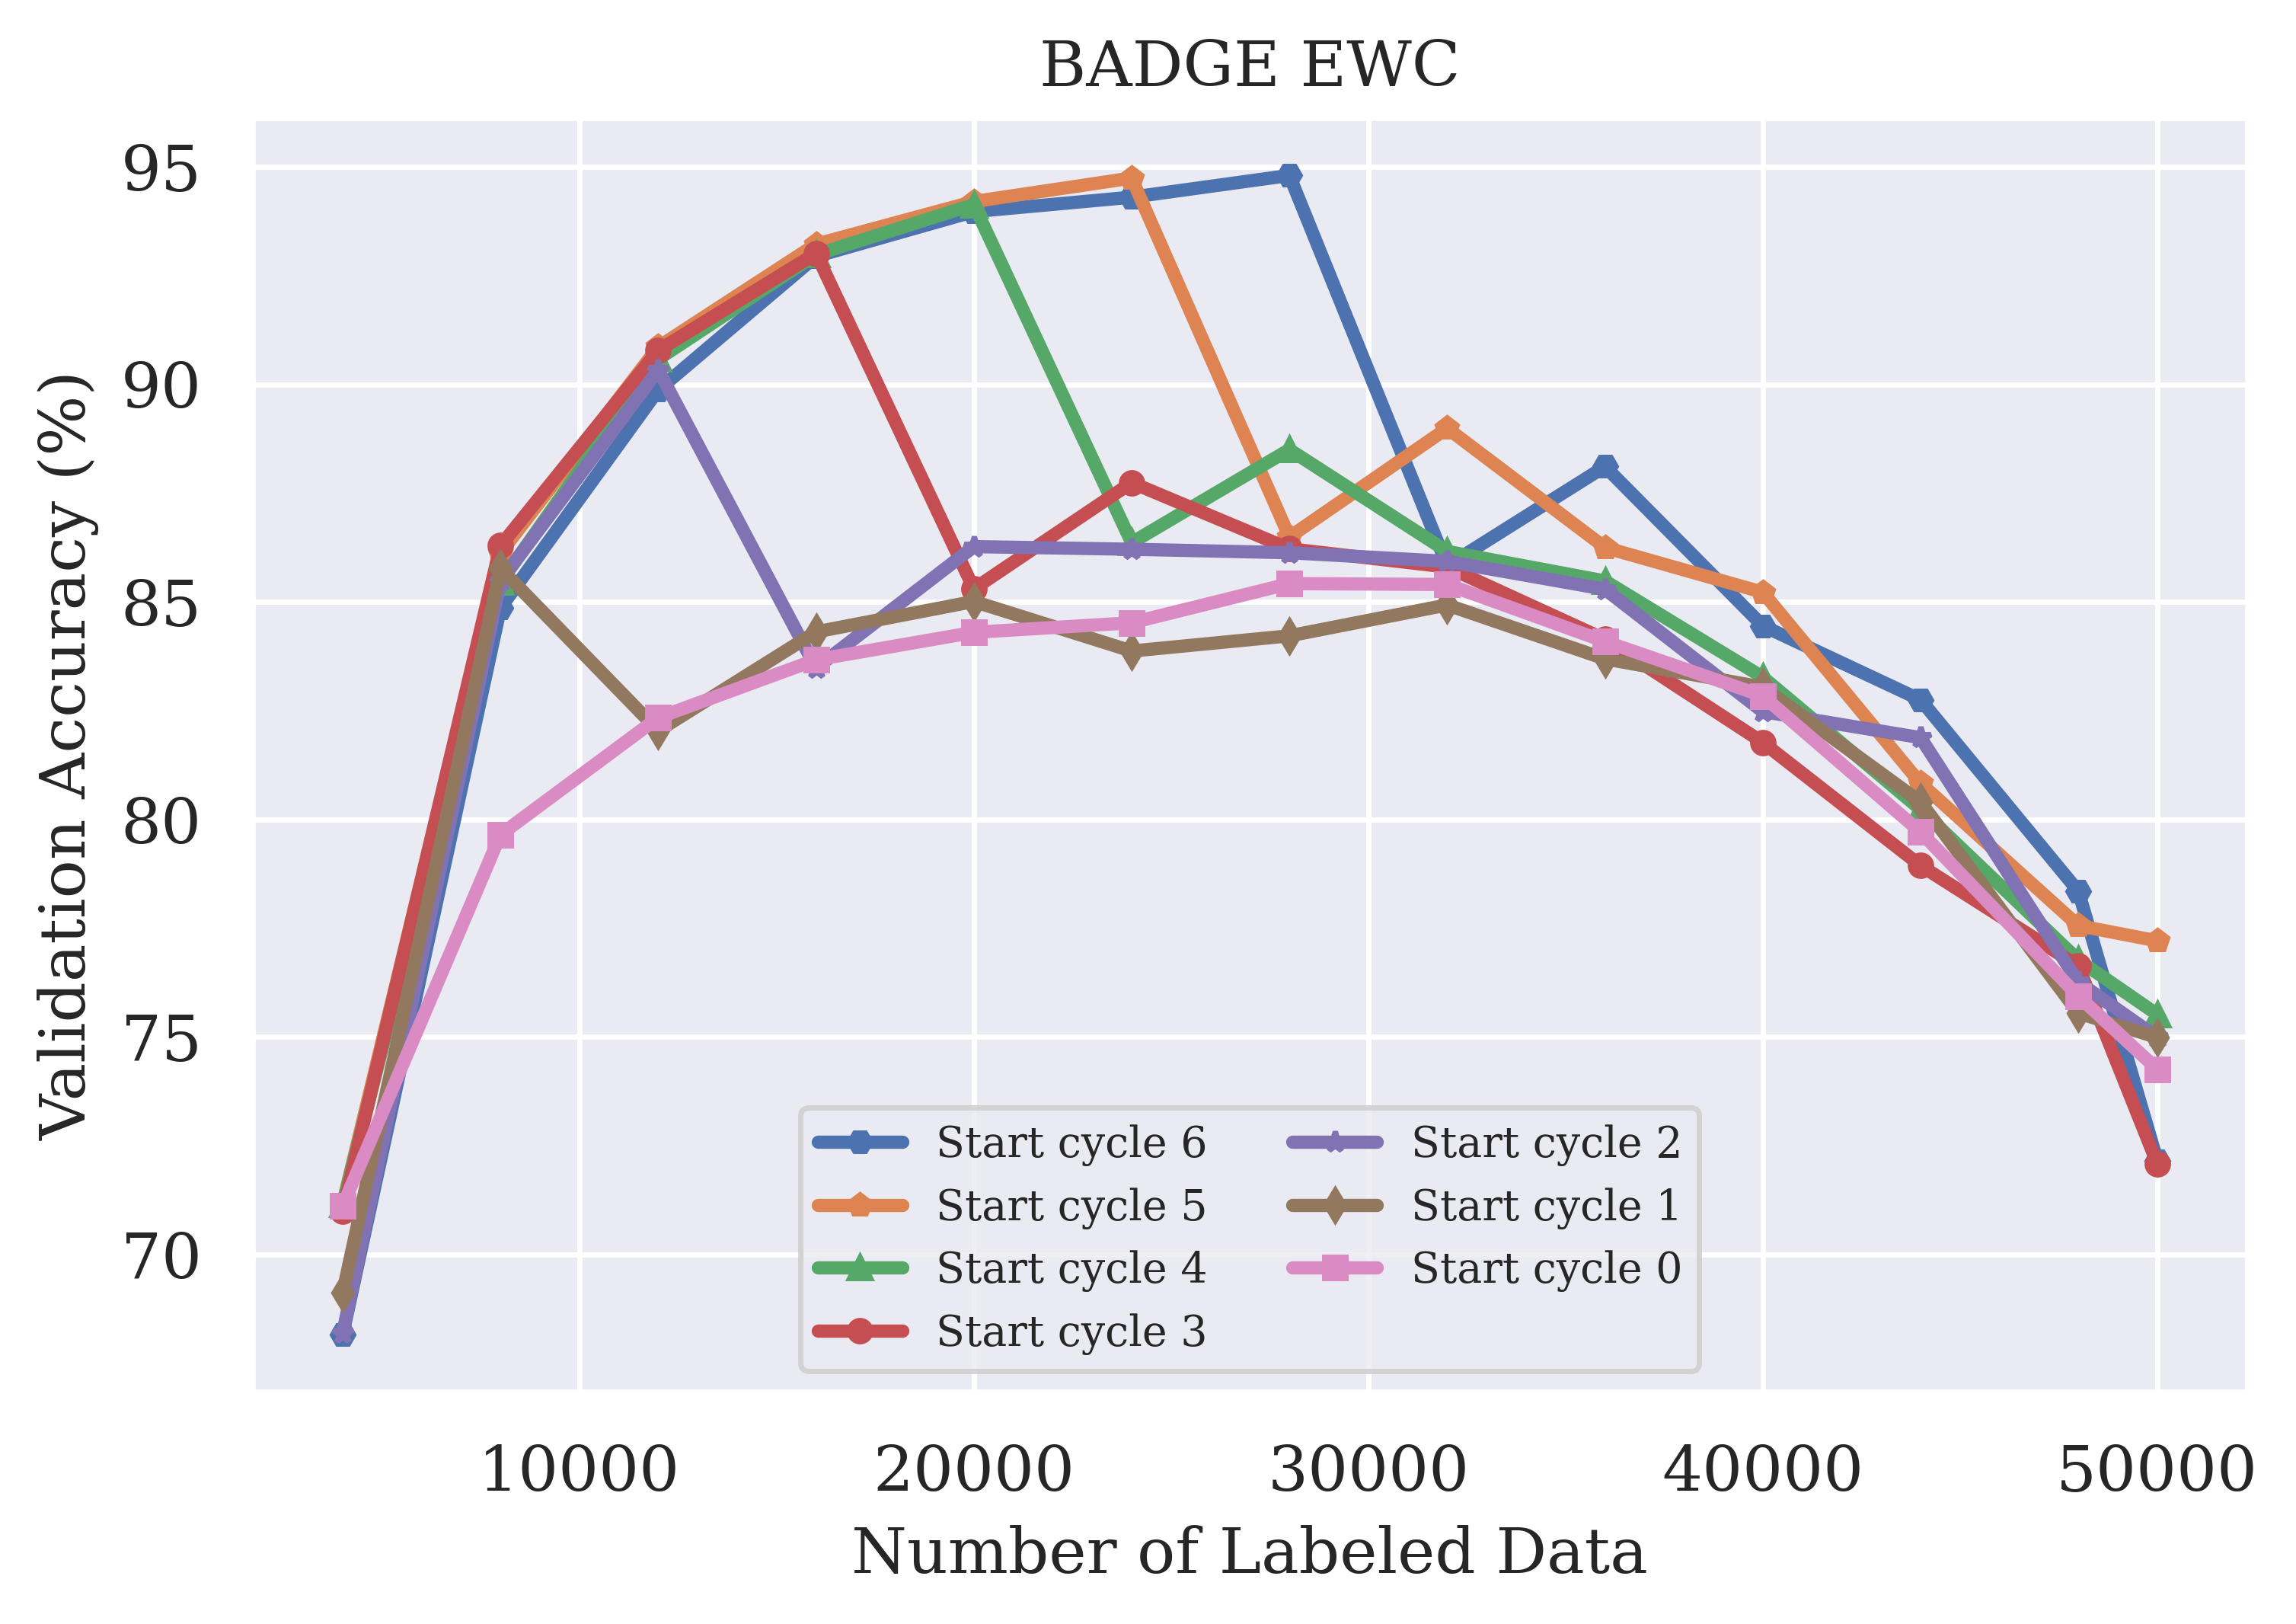
\includegraphics[width=0.45\linewidth]{images/results_CAL/delayed_start_badge_ewc.png} \hfill
    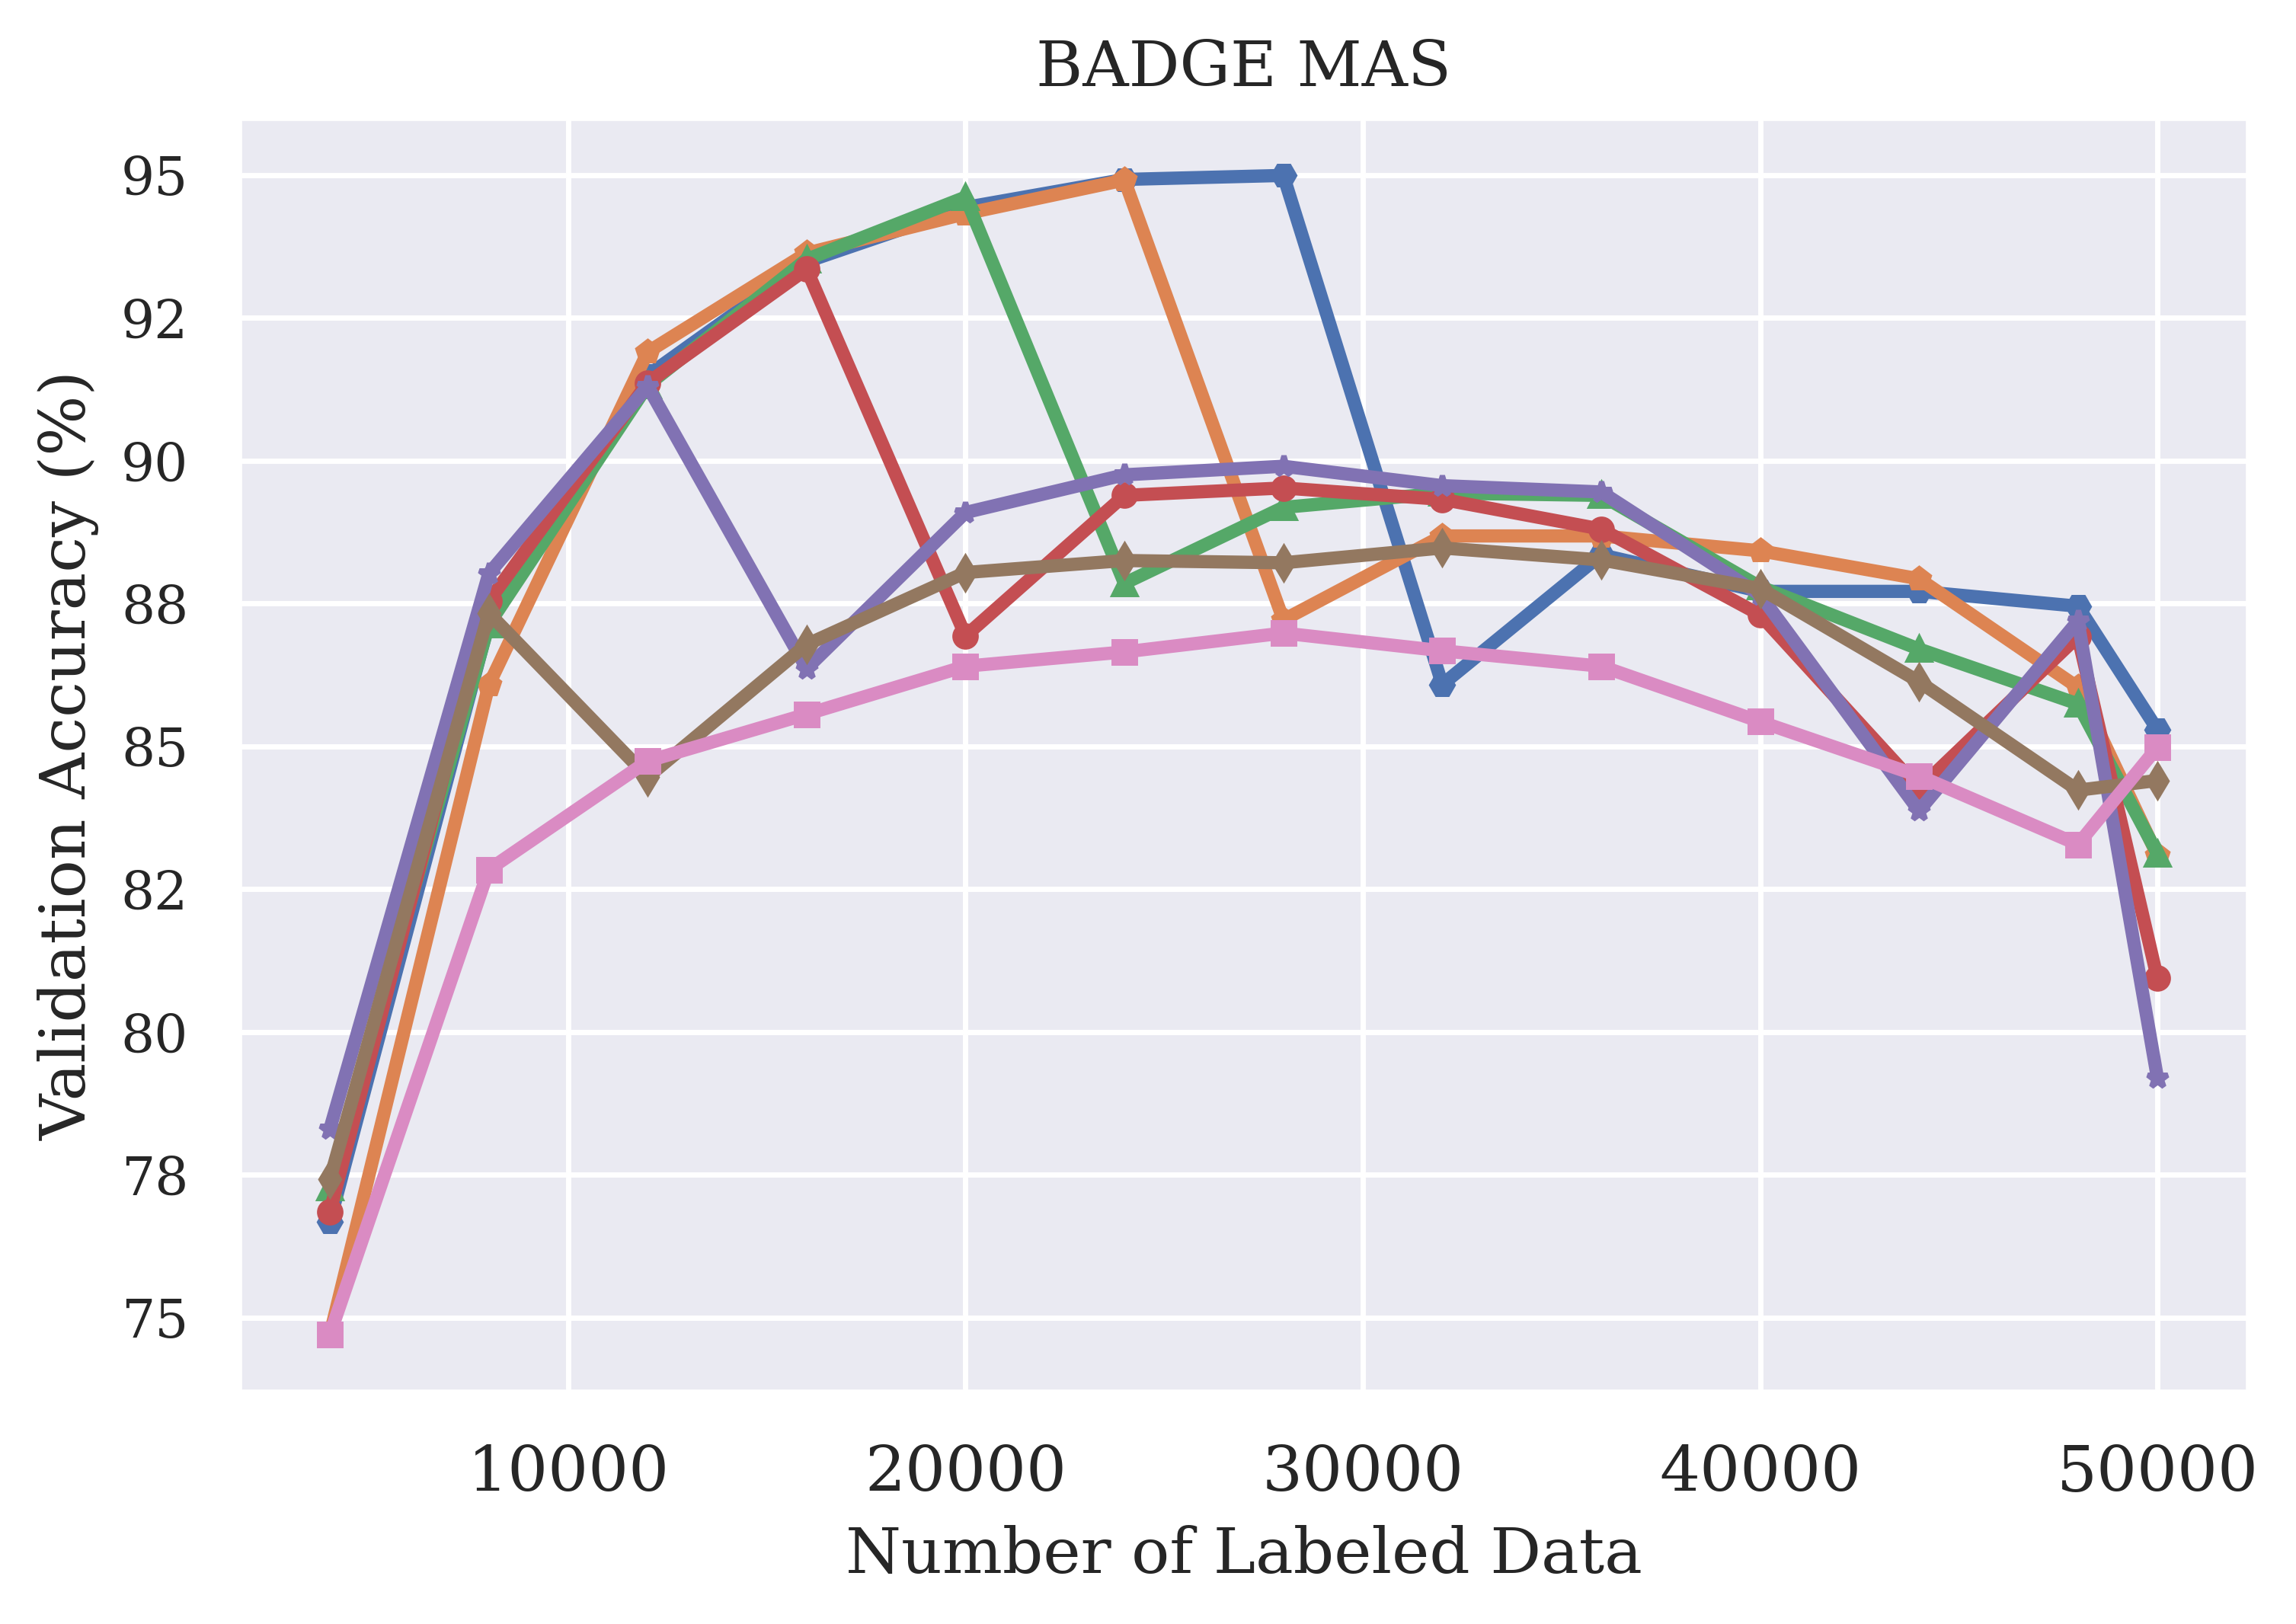
\includegraphics[width=0.45\linewidth]{images/results_CAL/delayed_start_badge_mas.png}
    \caption[Continual Active Learning Hybrid approach]{Comparison of validation accuracy for a delayed start of Continual Learning. Left: Accuracy progression for \gls{badge} and \gls{ewc}. Right: Accuracy progression for \gls{badge} and \gls{mas}.}
    \label{fig:Evaluation:Results:CAL:DelayedStart}
\end{figure}

\subsubsection{Varying the initialization of the labeled pool}
\label{sec:Evaluation:Results:CAL:Initialization}
Motivated by the findings from the previous section, we wonder if the initialization of the labeled pool has an impact on the validation accuracy of the Continual Learning strategies. Beck et al.\cite{beck2021effective} show that using a facility location selection 
\cite{iyer2021submodular} yields better validation accuracy when training on the initial labeled pool. We therefore test the effect of an initialization using the facility location selection compared to our random initialization. As our Active Learning strategy,
we use \gls{badge} with a batch size of 4000 and \gls{mas} as our Continual Learning strategy. The results of the experiment can be found in figure \ref{fig:Evaluation:Results:CAL:FLinit}. While the facility location approach performs better than random initialization, the difference is
marginal. Interestingly, the validation accuracy of the facility location approach is lower than the random initialization in the first iteration. The most significant drawback of the facility location initialization is its resource-intensity. Initialization with facility
location takes about 24 hours to complete and requires more than 100GB of memory for CIFAR-10 using the implementation provided by Beck et al. \cite{beck2021effective}. \par

\begin{figure}[h]
    \centering
    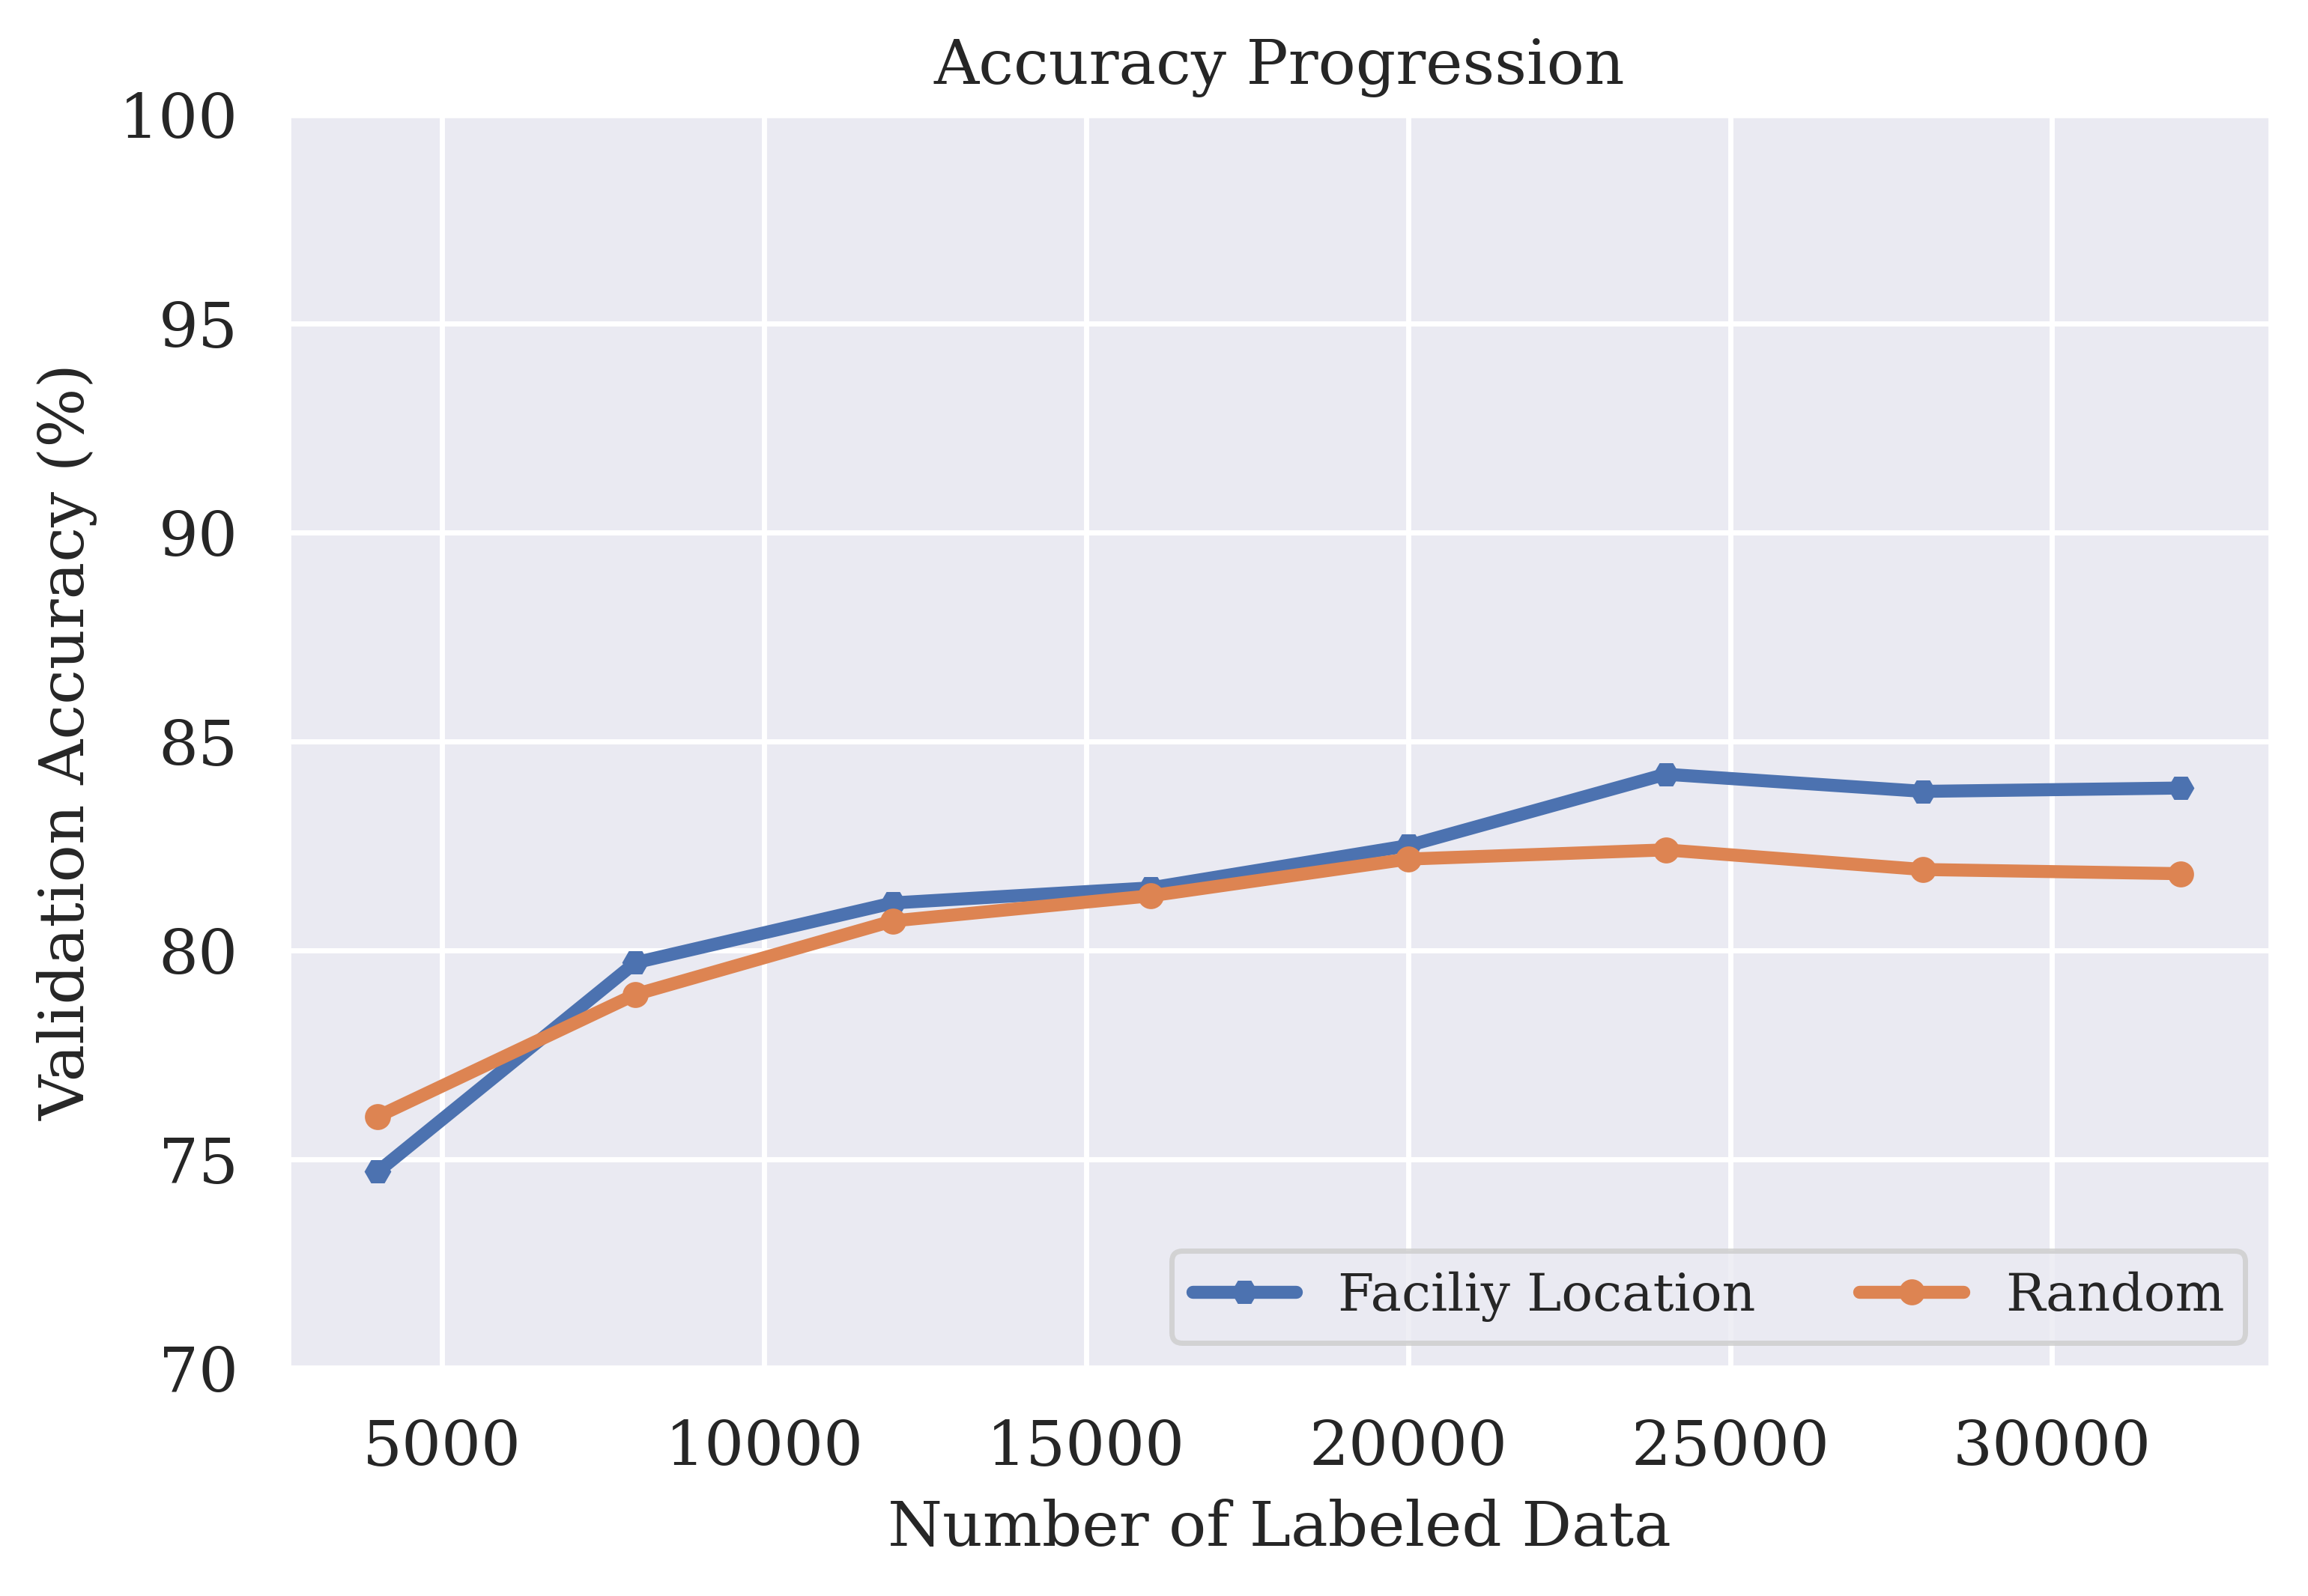
\includegraphics[width=0.7\linewidth]{images/results_CAL/Facility_location_init.png}
    \caption[Initialization using Facility Location]{Comparison of validation accuracy for facility location initialization and random initialization. We use a batch size of 4000 and the combination of \gls{badge} and \gls{mas} for the experiments.}
    \label{fig:Evaluation:Results:CAL:FLinit}
\end{figure}


\subsection{Replay Continual Learning}
\label{sec:Evaluation:Results:CAL:Replay}
In section \ref{sec:Methodology:ReplayStrategy} we introduced a custom replay strategy for Continual Active Learning. The use of our replay strategy is motivated by the main finding of section \ref{sec:Evaluation:Results:CAL:ALCL}: the validation accuracy increases with an
increased batch size. In this set of experiments, we use the Active Learning strategy CoreSet and vary the batch size and the size of the replay buffer. Moreover, we investigate the effect of CoreSet selection in the replay buffer compared to random selection. We present our
results in figure \ref{fig:Evaluation:Results:CAL:Replay}. When varying the batch size and buffer size, we notice that increasing the buffer size and the batch size yields a higher validation accuracy. However, our replay strategy does not outperform the Naive approach when using
the same amount of training data (i.e. batch size + replay buffer size for the replay strategy and batch size for the Naive approach). To evaluate the importance of CoreSet selection in the buffer compression process, we compare the validation accuracy of our replay strategy
when using CoreSet selection and random selection. We notice that the validation accuracy remains largely the same for both buffer compression methods, apart from the last 15000 samples, where CoreSet selection outperforms random selection. \par

%TODO: Hier die Bilder noch ändern sodass sie nicht aus Powerpoint sind
\begin{figure}[h]
    \centering
    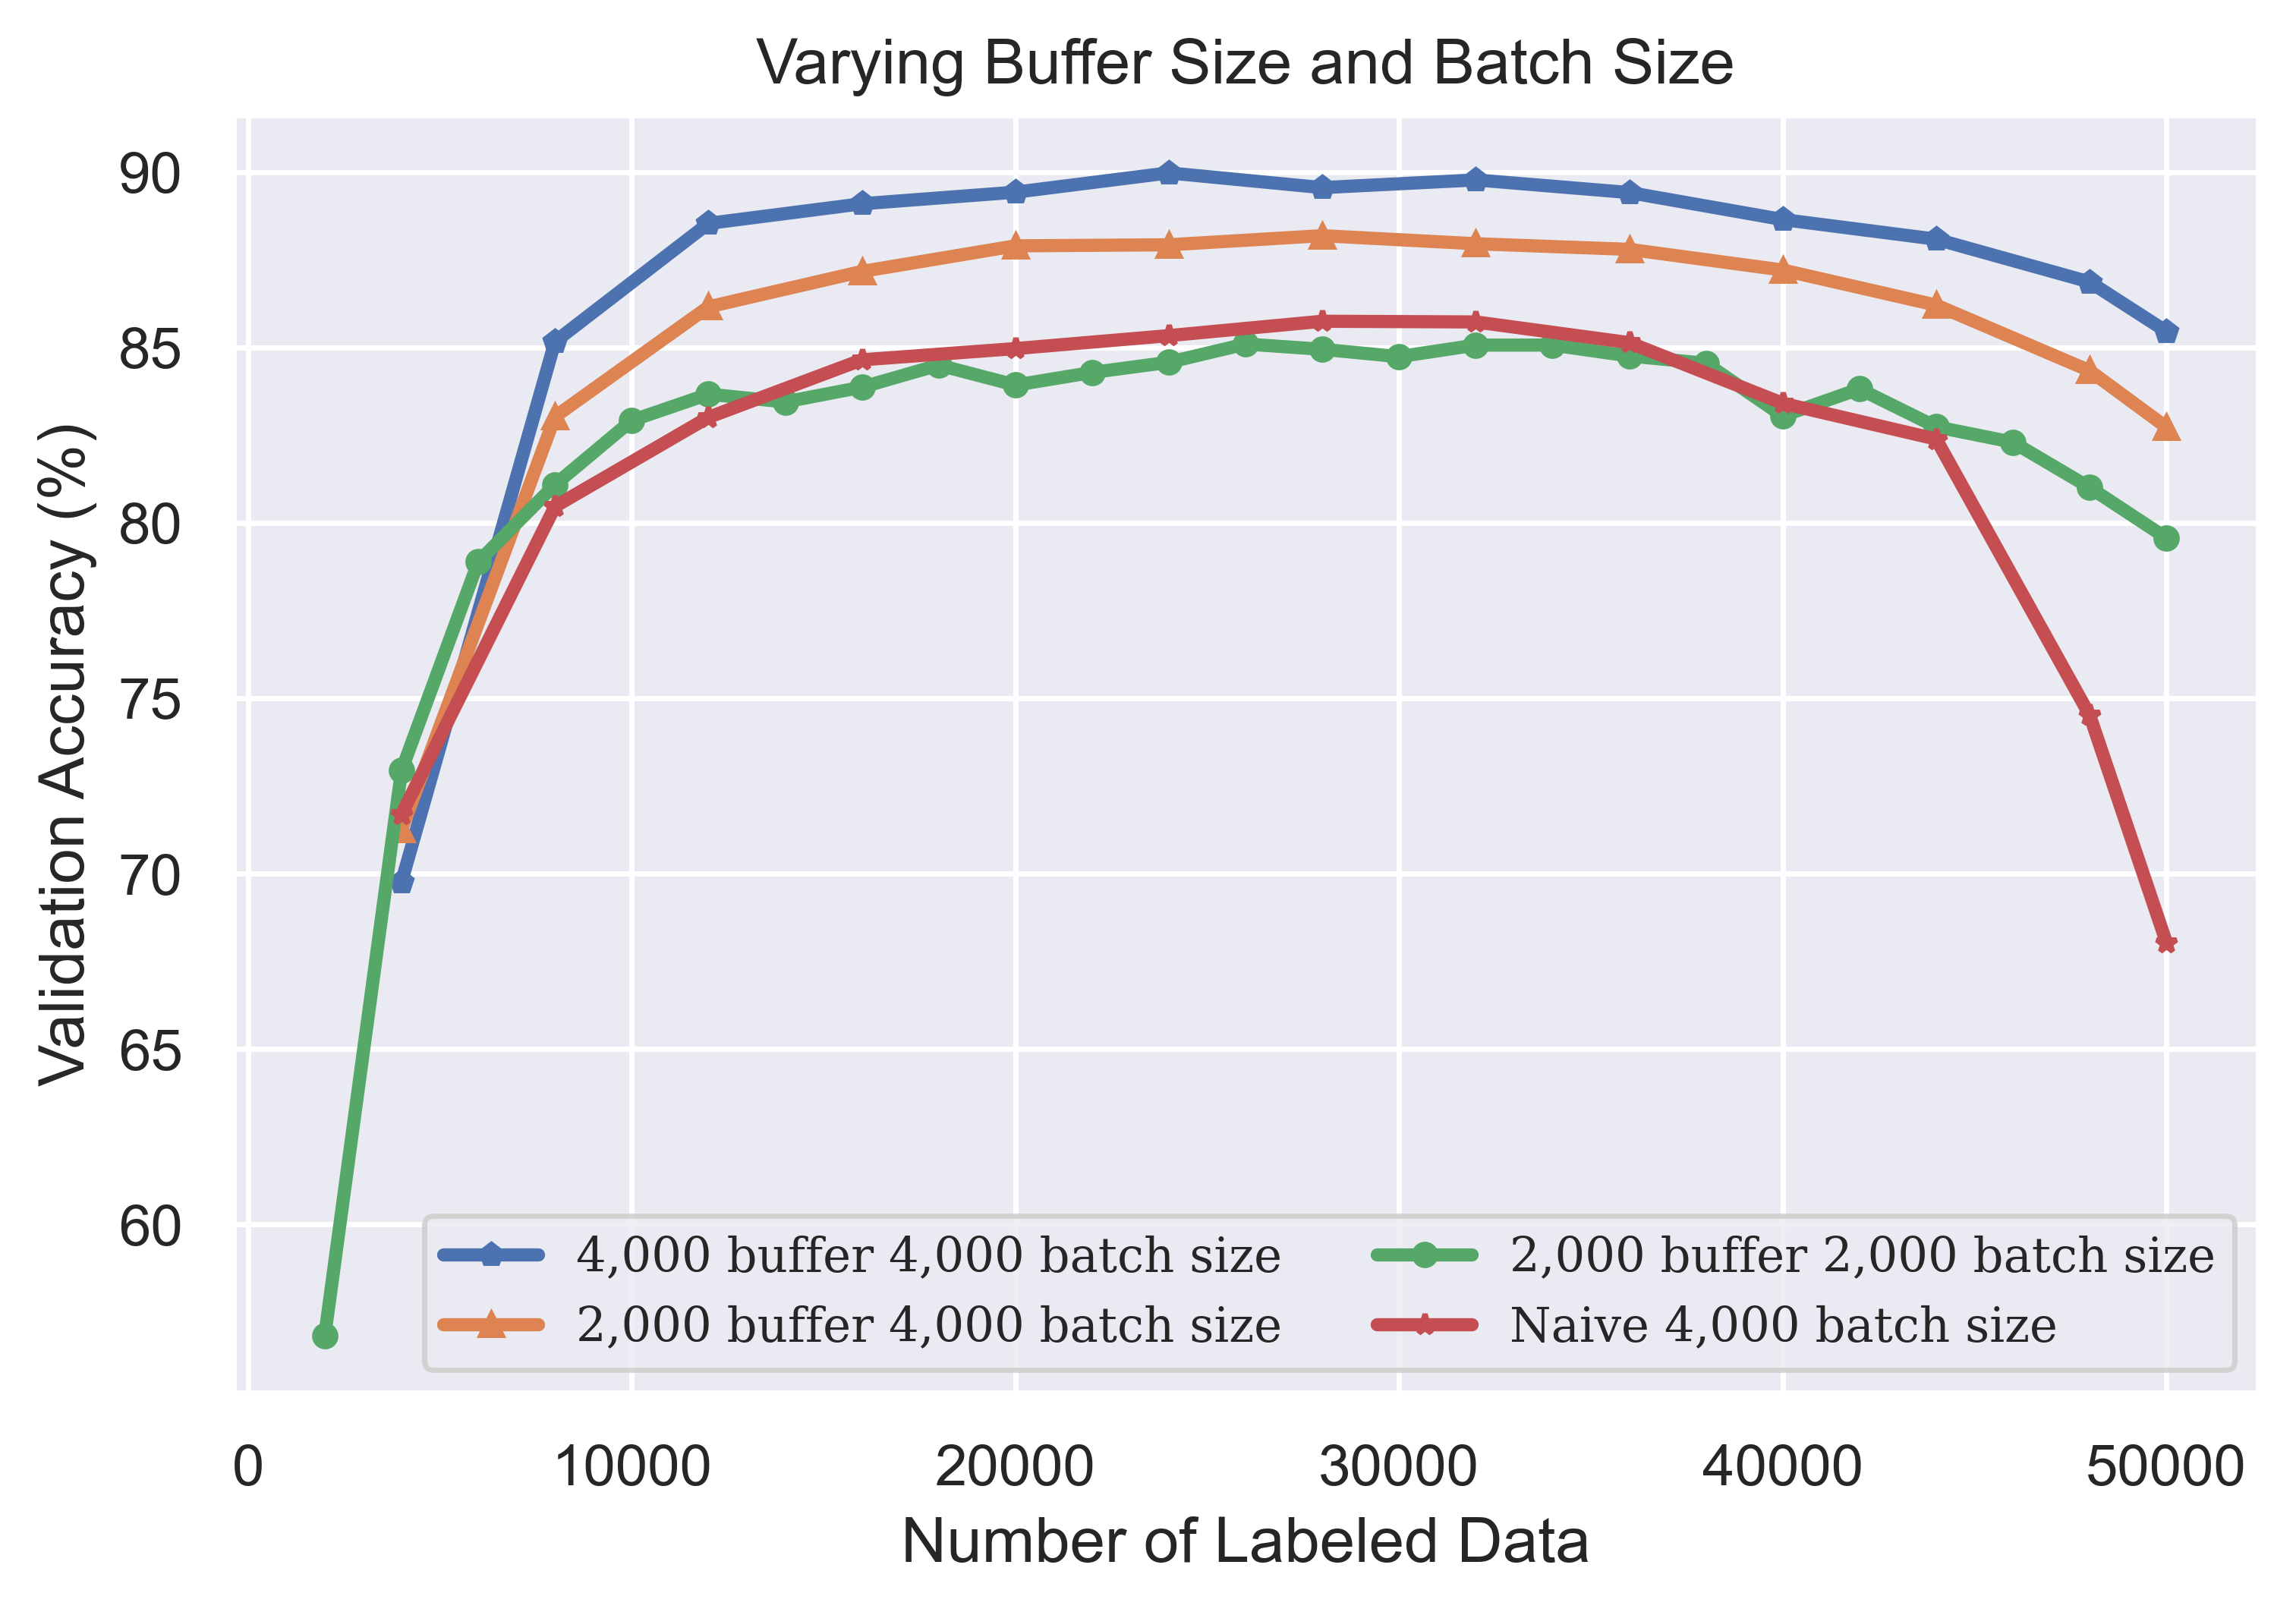
\includegraphics[width=0.45\linewidth]{images/results_CAL/replay_varying_batch_size.png} \hfill
    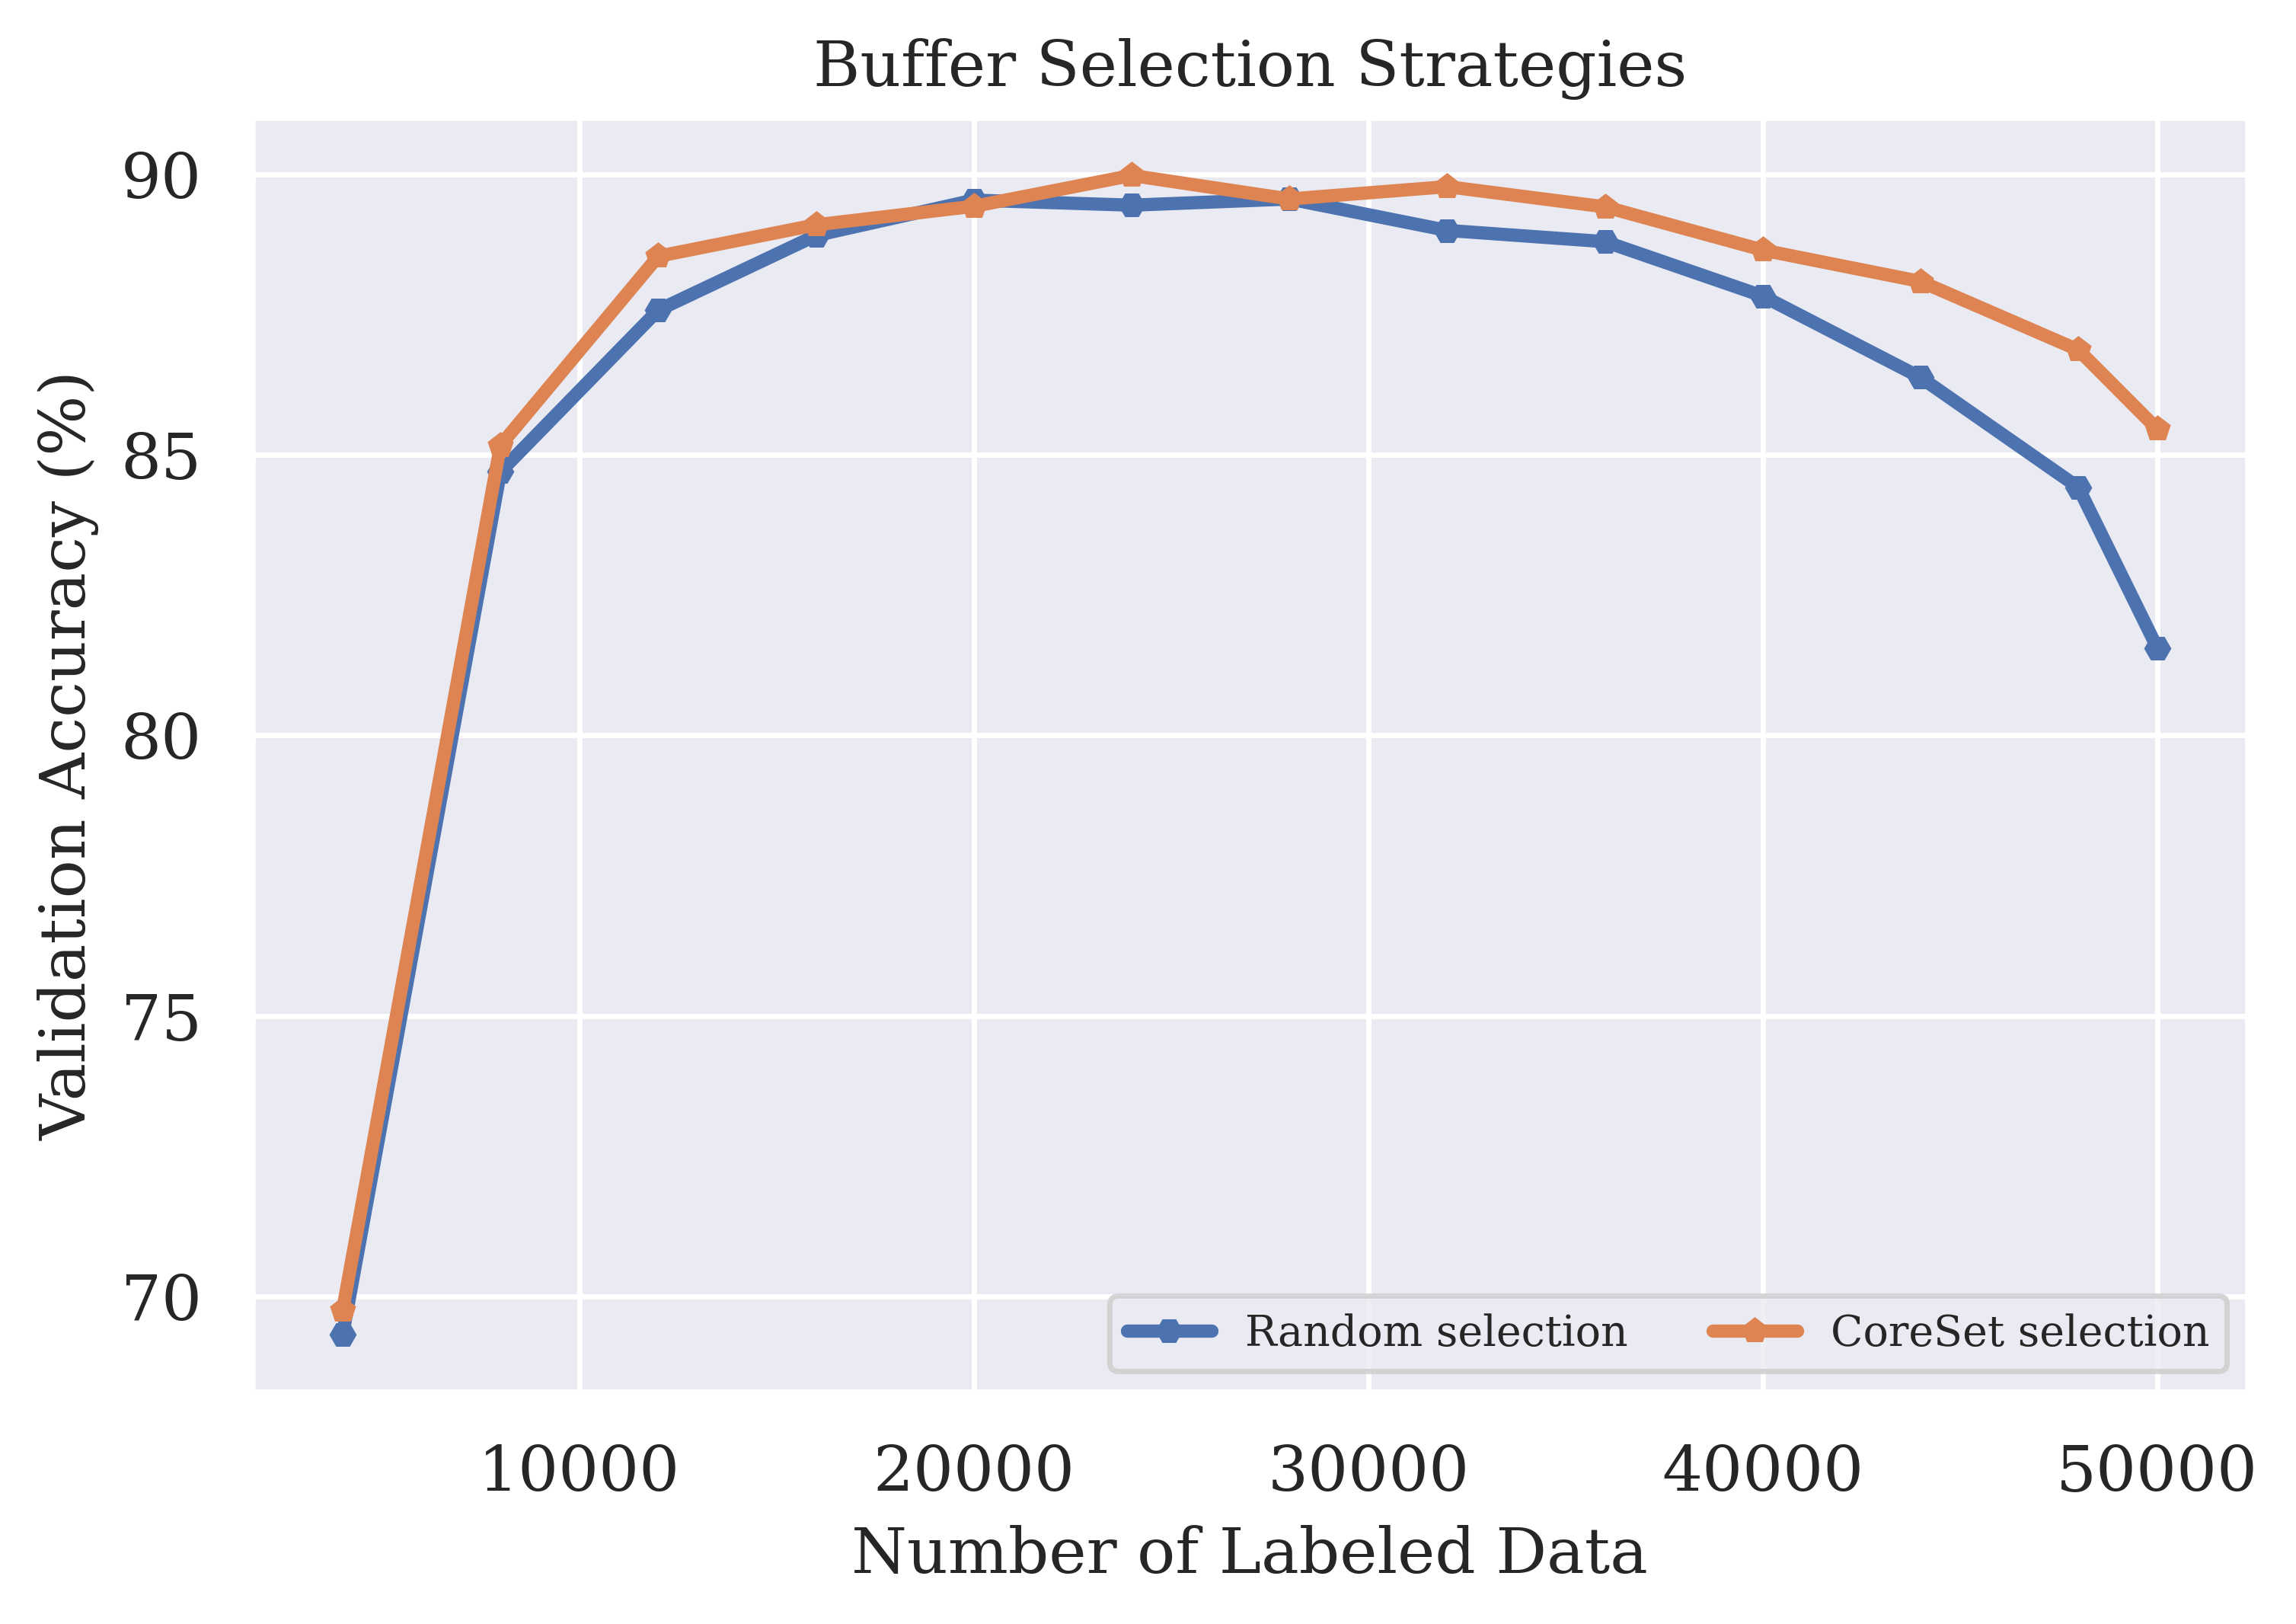
\includegraphics[width=0.45\linewidth]{images/results_CAL/replay_buffer_selection.png}
    \caption[Continual Active Learning Custom Replay strategy]{Left: Comparison of validation accuracy of our Replay strategy with different hyperparameters. Right: Comparison of validation accuracy of our Replay strategy when using different buffer compression approaches.
    In both runs, we use a batch size of 4000 and a replay buffer size of 4000.}
    \label{fig:Evaluation:Results:CAL:Replay}
\end{figure}

\subsection{Exemplar Rehearsal Continual Learning and Representation-based Active Learning}
\label{sec:Evaluation:Results:CAL:VAAL_AGEM}
Unsatisfied with the results from previous experiments, we decide to implement further Continual and Active Learning strategies. We perform an extensive literature search, investigating the suitability of representation-based Active Learning strategies and Continual Learning
strategies from the Exemplar Rehearsal category in the summary paper by Mundt et al. \cite{mundt2020wholistic}. The Active Learning strategy which we implement is \gls{vaal} \cite{sinha2019variational} and the Continual Learning strategy is \gls{a-gem} \cite{chaudhry2018efficient}. We decide
to implement \gls{vaal} because it is the only representation-based Active Learning strategy which consistently performs better than random sampling. The reason why we choose to implement \gls{a-gem} as our Continual Learning strategy is that is one of the few Exemplar Rehearsal strategies
applicable to (Semi-) supervised Learning (many other strategies focus on Reinforcement Learning) while being computationally efficient and demonstrating strong performance in the experiments by Chaudhry et al. \cite{chaudhry2018efficient} at the same time. \par
First, we analyze the performance of \gls{vaal} as an Active Learning strategy. We run \gls{vaal} with a batch size of 4000 and compare it to Random and CoreSet. We choose Random because it is the baseline for Active Learning strategies and CoreSet because it is among the best performing Active
we used before. The results can be found in the left plot in figure \ref{fig:Evaluation:Results:CAL:VAAL}. While \gls{vaal} outperforms random sampling by a large margin, it is itself outperformed by about the same margin by Coreset. To ensure that the results are not due to a
suboptimal hyperparameter choice, we run \gls{vaal} training VAE and Discriminator for 20 epochs in one run and 100 epochs in another. Because we are interested in the performance of \gls{vaal} in our Continual Active Learning setting, we use Continual Active Learning with a batch size of 4000
and the Continual Learning strategy Naive. We present the results of the experiment in the right plot of figure \ref{fig:Evaluation:Results:CAL:VAAL}. Surprisingly, the validation accuracy is marginally impacted by the training time of Generator and VAE. If anything, the validation
accuracy is higher when training for 20 epochs. \par

\begin{figure}[h]
    \centering
    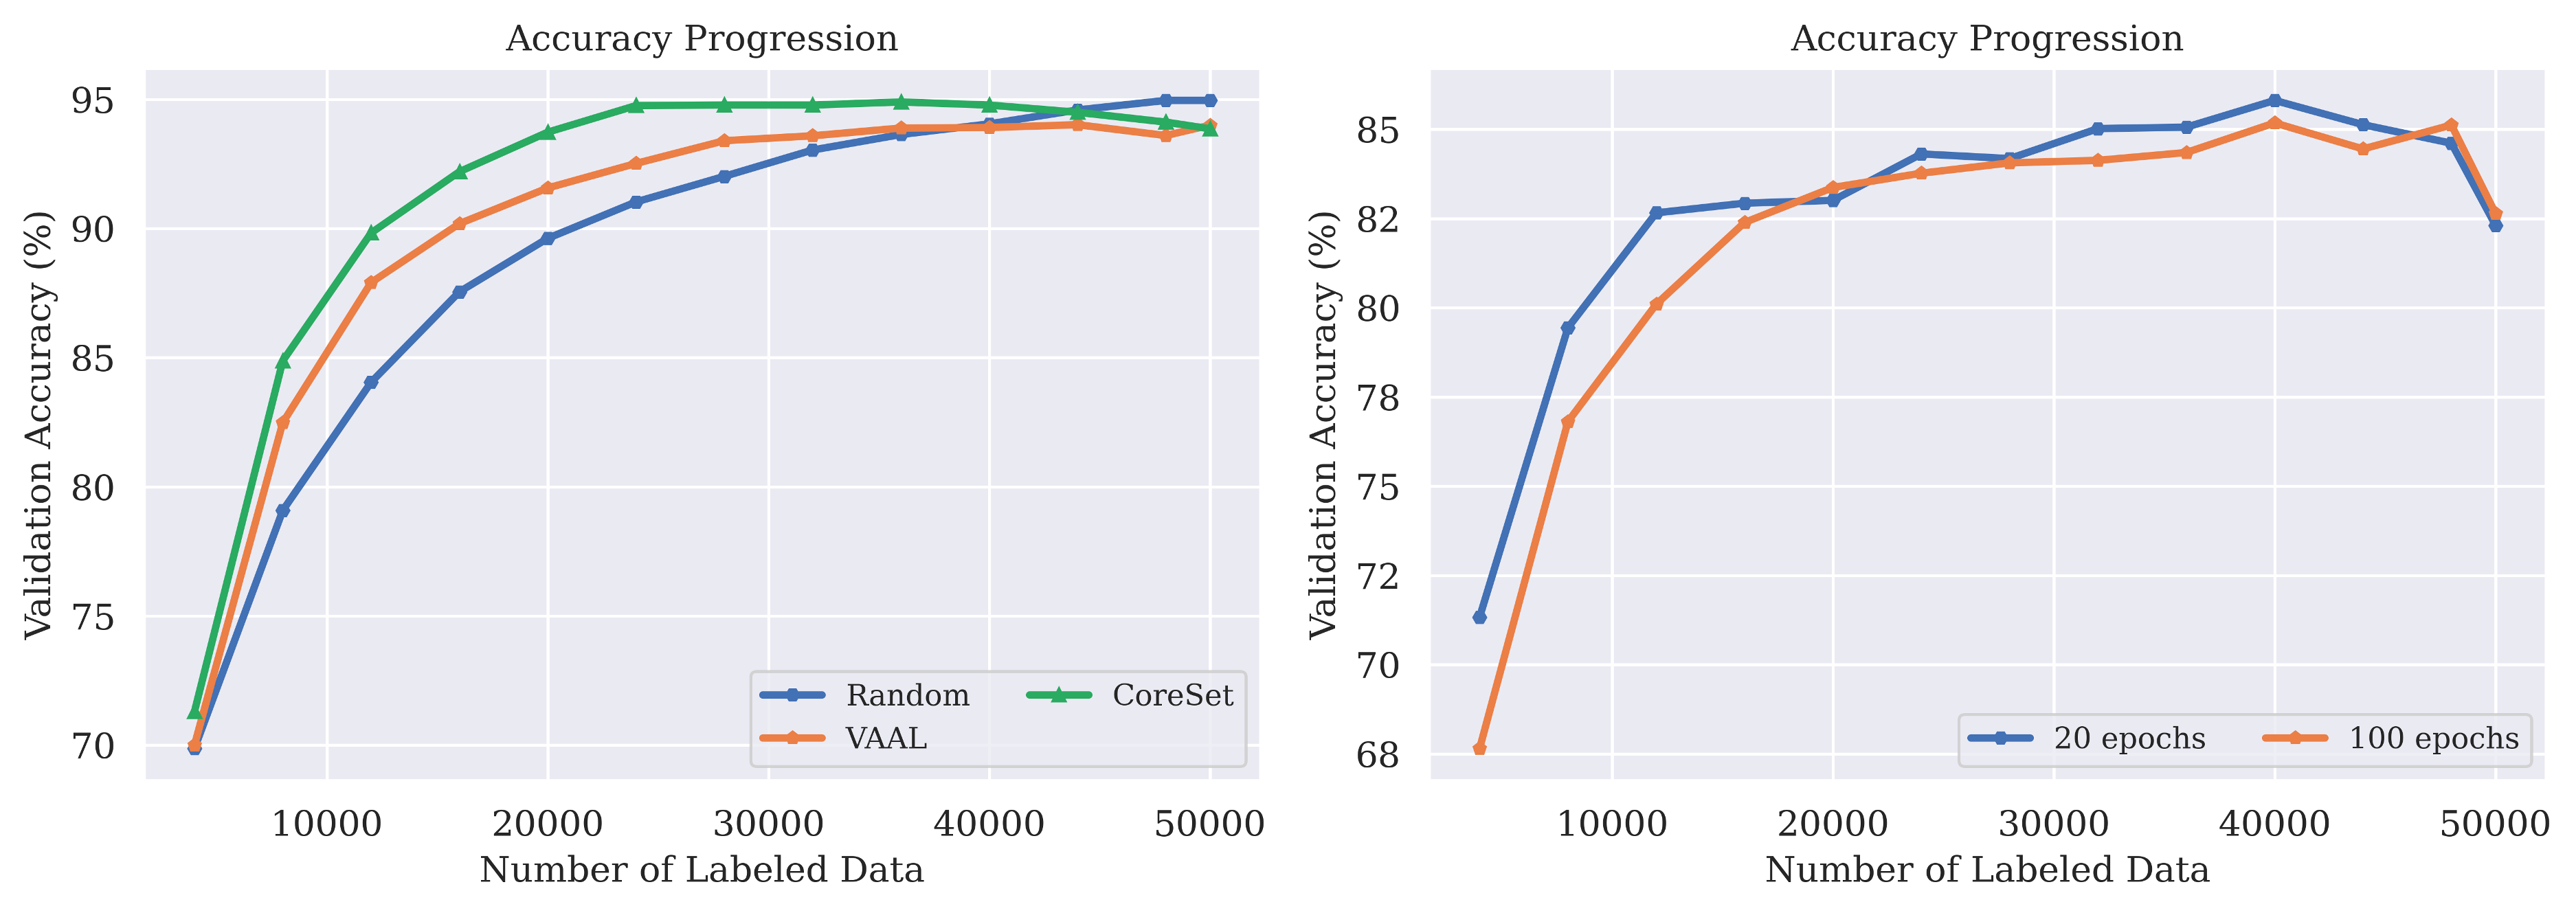
\includegraphics[width=\linewidth]{images/results_CAL/VAAL_plots.png}
    \caption[Continual Active Learning Custom Replay strategy]{Left: Comparison of validation accuracy of \gls{vaal} to the Active Learning strategies Random and CoreSet. We use a batch size of 4000 for the experiments. Right: Comparison of validation accuracy when varying the training 
    epochs for \gls{vae} and Discriminator. We use Continual Active Learning with the Naive approach as our Continual Learning strategy and a batch size of 4000.}
    \label{fig:Evaluation:Results:CAL:VAAL}
\end{figure}

Next, we experiment with \gls{a-gem}. \gls{a-gem} has two hyperparameters: $S$, which is the number of samples randomly drawn from the memory to compute the reference gradients and $P$ which is the number of data points stored to the memory from each task. We run \gls{a-gem} with the Active Learning
strategy \gls{lc} and a batch size of 2000. To assess the performance of \gls{a-gem}, we compare its validation accuracy to the Naive approach. We vary $S$ and $P$ and present our results in the right plot of figure \ref{fig:Evaluation:Results:CAL:AGEM}. The validation accuracy increases with
an increased $S$ and $P$ until about 12000 samples, after which the validation accuracy drops for all values of $S$ and $P$. \gls{a-gem} outperforms the Naive approach for the first 15000 samples, but is outperformed by Naive for the remainder of the experiment. \par
After investigating the influence of \gls{a-gem}'s hyperparameters, we compare the combination of \gls{vaal} and \gls{a-gem} to \gls{vaal} and Naive, using a batch size of 4000. The results are shown in the left plot of figure \ref{fig:Evaluation:Results:CAL:AGEM}. Although \gls{a-gem} performs worse than the Naive
approach when using the Active Learning strategy \gls{lc}, it outperforms the Naive approach when using \gls{vaal} as the Active Learning strategy. \par

\begin{figure}[h]
    \centering
    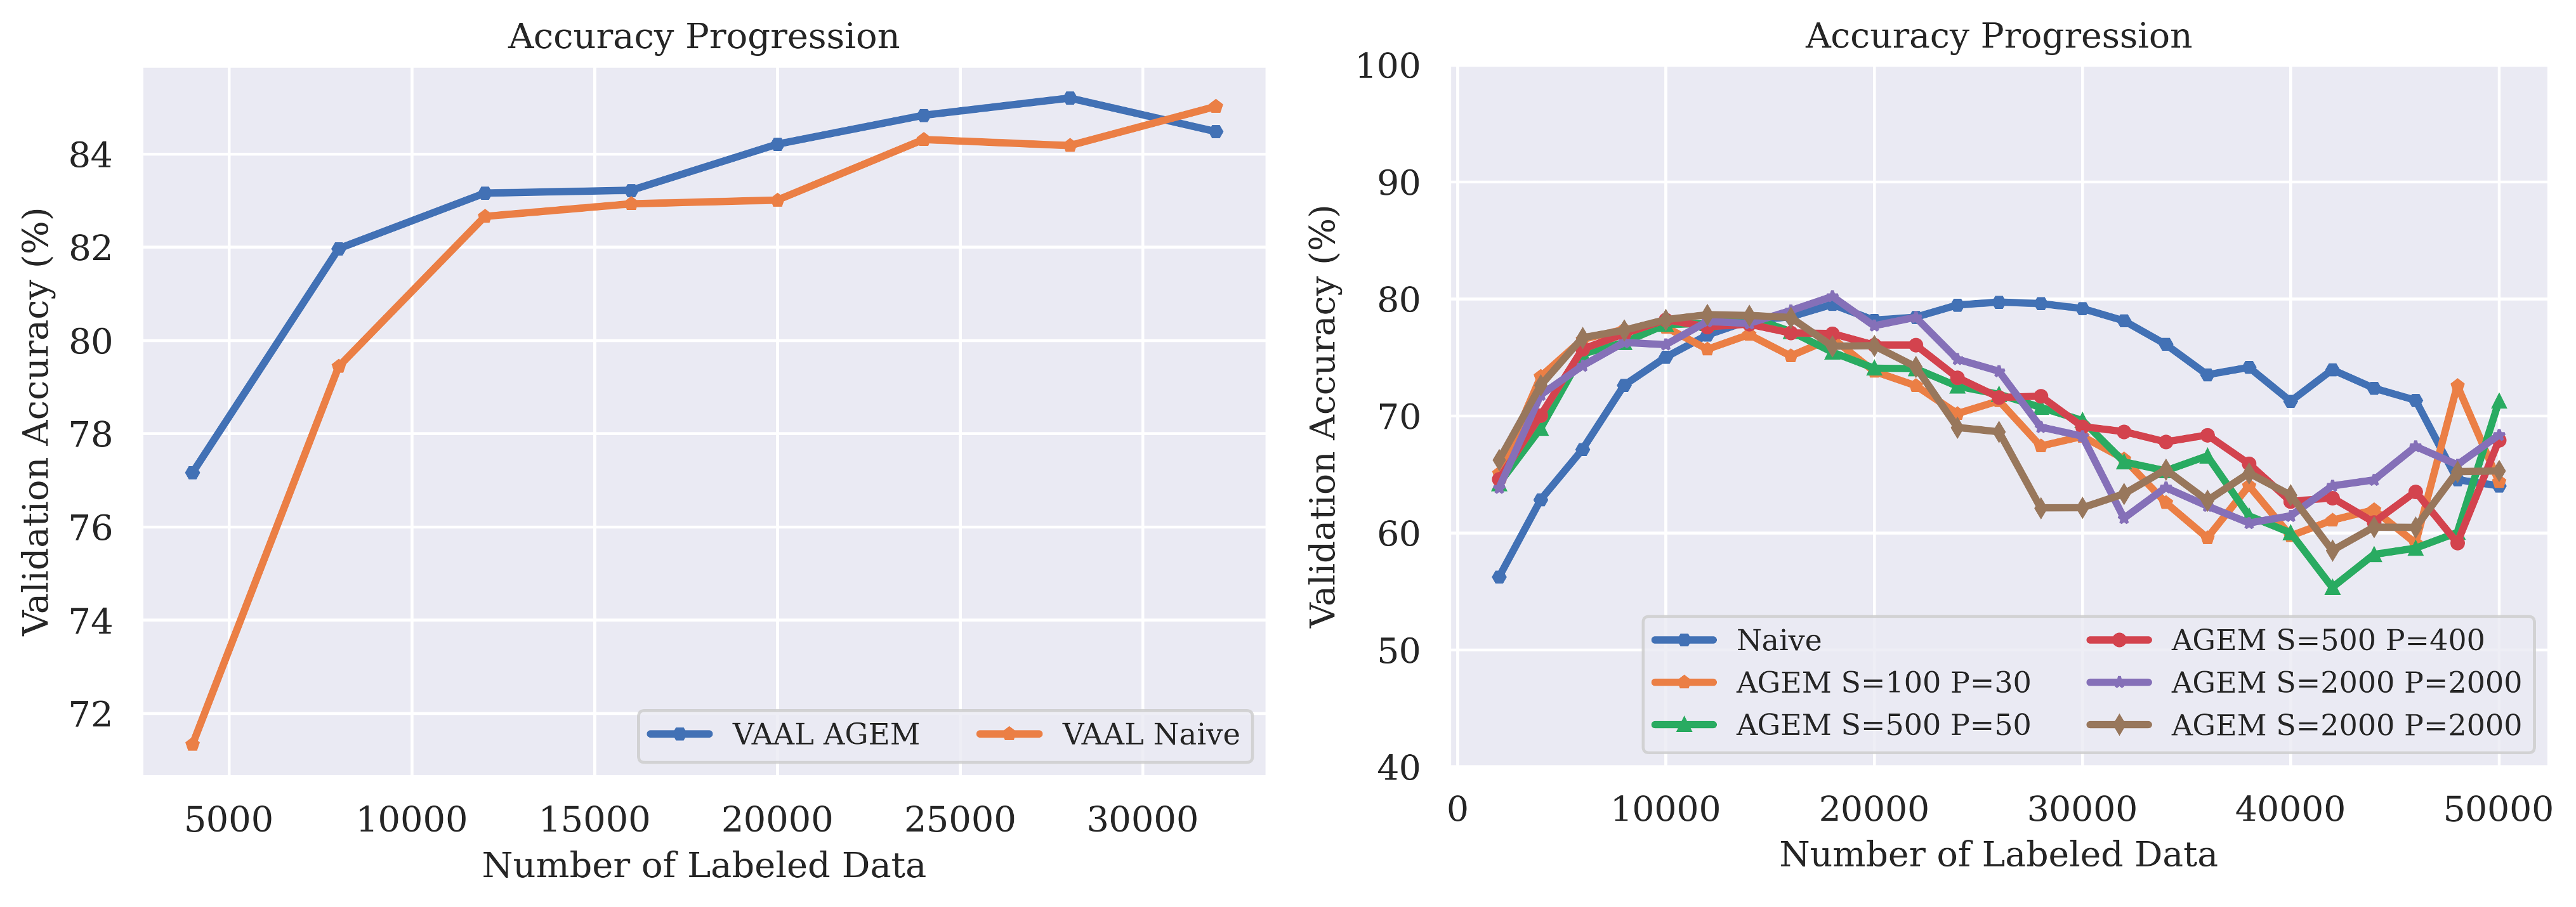
\includegraphics[width=\linewidth]{images/results_CAL/AGEM_plots.png}
    \caption[Continual Active Learning Custom Replay strategy]{Left: Comparison of validation accuracy of \gls{a-gem} to the Naive approach when using \gls{vaal} as the Active Learning strategy We use a batch size of 4000 for the experiments. Right: Comparison of validation accuracy of \gls{a-gem}
     to the Naive approach when using different values of $S$ and $P$. We use the Active Learning strategy \gls{lc} and a batch size of 2000 for the experiments.}
    \label{fig:Evaluation:Results:CAL:AGEM}
\end{figure}


\begin{table}[h]
    \centering
    \begin{tabular}{c | c } 
        Batch Size & \gls{vaal}\\ 
        \hline 
        Baseline & 961 \\
        Naive & 341 \\
        \gls{a-gem} & 862 \\
    \end{tabular}
    \caption{Comparison of execution time using \gls{vaal}}
    \label{fig:Evaluation:CAL:VAAL_AGEM_Time}
\end{table}

\section{Continual Active Learning for Model Stealing}
\label{sec:Evaluation:Results:MS}
After extensively studying Continual Active Learning, we shift the focus of our experiments to Model Stealing. Since we build our work on the ActiveThief framework, we first evaluate the performance of the ActiveThief framework, including the influence of Model Architecture and
Thief Dataset as well as the difference between stealing a target model returning the predicted labeled and stealing a target model returning the softmax outputs of the final model layer. After experimenting with the ActiveThief framework, we evaluate the performance of our pro
-posed Continual Active Learning strategy for Model Stealing attacks. We perform the experiments on the MNIST, CIFAR-10 and CIFAR-100 datasets and end with a decisive insight on the effect of data augmentation for Model Stealing attacks. \par


\subsection{Regularization-based Continual Learning}
\label{sec:Evaluation:Results:MS:Regularization}


In this section, we evaluate the success of Model Stealing Attacks using Continual Active Learning. More specifically, we run Model Stealing Attacks with Continual Active Learning on the datasets MNIST, CIFAR-10 and CIFAR-100, using the Active Learning strategies
Random, \gls{lc}, \gls{bald}, \gls{badge} and CoreSet and the Continual Learning strategies Naive, \gls{ewc}, \gls{imm}, \gls{mas} and \gls{alasso}. Furthermore, we differentiate between receiving the softmax output of the target model and solely receiving the top1-label. We use the ActiveThiefConv3 model
as the target and substitute model and perform one model stealing attack for each combination of Active Learning, Continual Learning strategy and target model output. For the baseline runs, we use a batch size of 1000 with a total query budget of 20000. The query budget
is kept for the Continual Active Learning runs, but we increase the batch size to 2000. The numbers reported in the table represent the model agreement at the end of each experiment, i.e. after using up the query budget of 20000. Readers interested in the progression of the
model agreement across the experiments can find the respective plots in appendix \ref{sec:Appendix:Results}. As a baseline we use the Model Extraction using Active Learning with the strategies mentioned before. To evaluate both the Active Learning strategies and the Continual
Learning strategies, we compute the average over the model agreement of all Continual Learning strategies combined with a fixed Active Learning strategy and the average of all Active Learning strategies combined with a fixed Continual Learning strategy. These numbers are given
at the end of each column and row, respectively. The Active Learning strategy and the Continual Learning strategy with the highest average model agreement are highlighted in bold. \par
In the first set of experiments, we perform Model Stealing Attacks using Continual Active Learning with MNIST as our target model and train the substitute model on the softmax output of the target model. The results of this experiment can be found in table
\ref{fig:ModelStealingMNISTSoftmax}. In terms of model agreement, all Continual Active Learning attacks perform significantly worse than the baseline. The best performing attack is the combination of the Active Learning strategy \gls{bald} with the Continual Learning strategy
\gls{mas} with a model agreement of 67.84\% after a query budget of 20000. The best performing Active Learning strategy is \gls{bald} with an average model agreement of 52.52\% across all Continual Learning strategies whereas the best Continual Learning strategy is \gls{mas} with an average
model agreement of 57.73\%. While the Continual Learning strategies struggled to outperform the Naive approach in the classic Continual Active Learning setting, most of them outperform the Naive approach in the Model Stealing setting. The only exception to this is \gls{alasso} which
falls behind the other approaches significantly. \par 

\begin{table}[h]
    \centering
    \begin{tabular}{ c | c c c c c | c } 
         & Random & \gls{lc} & \gls{bald} & CoreSet & \gls{badge} & $\varnothing$\\ 
        \hline
        Naive & 47.74 & 43.02 & 59.61 & 58.36 & 48.89 & 51.52\\
        \gls{ewc} &  59.26 & 53.67 & 59.18 & 56.13 & 50.28 & 55.7\\
        \gls{imm} & 48.18 & 62.95 & 49.71 & 63.43 & 58.76 & 56.61 \\
        \gls{mas} &  64.42 & 50.27 & 67.84 & 55.58 & 50.54 & \textbf{57.73}\\
        \gls{alasso} & 28.04 & 15.5 & 26.28 & 10.39 & 12.8 & 20.6\\
        \hline
        $\varnothing$ & 49.57 & 45.08 & \textbf{52.52} & 48.78 & 44.24 & /\\
        Baseline & 87.91 & 82.39 & 83.64 & 91.22 & 79.68 & 84.97\\
    \end{tabular}
    \caption{Model agreement of continual learning strategies on MNIST using softmax output}
    \label{fig:ModelStealingMNISTSoftmax}
\end{table}

Next, we change the output of the target model to solely return the top1-label and perform the same set of experiments. Table \ref{fig:ModelStealingMNISTLabel} shows the results of these experiments. While the model agreement compared to training with softmax output of the
target model has dropped significantly for the baseline strategies, we do not observed a similar phenomenon for the Continual Active Learning strategies. Nevertheless, we observe a large maring between the Model Agreement of the Active Learning strategies and the Model Agreement
of the Continual Active Learning strategies. However, the combination of \gls{bald} and Naive comes close to its baseline, demonstrating a Model Agreement of 69.18\% which is about 7 percentage points lower than the respective baseline. Overall, the Naive approach performs best with an
average Model Agreement of 51.29\% across all Active Learning strategies. Contrary to the previous setup, no Continual Learning strategy outperforms the Naive approach, with \gls{mas} coming closest. The best Active Learning strategy is \gls{bald} with an average Model Agreement of 55.73\%. \par 

\begin{table}[h]
    \centering
    \begin{tabular}{c | c c c c c | c } 
         & Random & \gls{lc} & \gls{bald} & CoreSet & \gls{badge} & $\varnothing$ \\ 
        \hline
        Naive & 43.44 & 58.84 & 69.18 & 44.88 & 40.12 & \textbf{51.29}\\
        \gls{ewc} &  46.76 & 47.3 & 52.36 & 36.84 & 44.73 & 45.6\\
        \gls{imm} & 47.07 & 10.43 & 58.71 & 51.0 & 47.0 & 42.84\\
        \gls{mas} & 50.52 & 46.79 & 49.51 & 44.96 & 49.47 & 48.25\\
        \gls{alasso} &  10.44 & 46.89 & 48.89 & 16.27 & 10.43 & 26.68\\
        \hline
        $\varnothing$ & 39.65 & 50.97 & \textbf{55.73} & 38.79 & 38.35 & /\\
        Baseline & 67.56 & 80.36 & 76.29 & 81.62 & 76.43 & 76.45\\
    \end{tabular}
    \caption{Model agreement of continual learning strategies on MNIST using the predicted class label}
    \label{fig:ModelStealingMNISTLabel}
\end{table}

We move on to the next dataset which is CIFAR-10. First, we perform Model Stealing attacks using the softmax output of the target model. Our results can be found in Table \ref{fig:ModelStealingCIFAR10Softmax}. Similar to our findings from the MNIST dataset, the Continual Active Learning
are outperformed by the Active Learning strategies, however the gap between is mostly consistent across combinations of Active and Continual Learning strategies at around 10 percentage points. \gls{alasso} is once again an exception to this, performing significantly worse than the other
Continual Learning strategies. The best Continual Active Learning strategy is \gls{ewc} with an average Model Agreement of 60.14\%. At the same time, \gls{ewc} is the only Continual Learning strategy to outperform the Naive approach, albeit the margin between the two is only 0.48 percentage points.
Overall, CoreSet is the most performant Active Learning strategy with an average model agreement of 54.12\% across all Continual Learning strategies. \par

\begin{table}[h]
    \centering
    \begin{tabular}{ c | c c c c c | c } 
         & Random & \gls{lc} & \gls{bald} & CoreSet & \gls{badge} & $\varnothing$\\ 
        \hline 
        Naive & 60.8 & 56.62 & 61.84 & 61.61 & 57.42 & 59.66 \\
        \gls{ewc} & 58.67 & 56.8 & 61.57 & 61.79 & 61.88 & \textbf{60.14}\\
        \gls{imm} & 60.78 & 52.24 & 60.32 & 61.39 & 56.98 & 58.34 \\
        \gls{mas} & 50.32 & 51.45 & 52.09 & 52.23 & 55.68 & 52.35\\
        \gls{alasso} & 17.26 & 24.87 & 28.24 & 33.59 & 32.93 & 27.38\\
        \hline
        $\varnothing$ & 49.57 & 48.4 & 52.81 & \textbf{54.12} & 52.98 & /\\
        Baseline & 71.58 & 70.04 & 71.96 & 71.45 & 71.44 & 71.29\\
    \end{tabular}
    \caption{Model agreement of Continual Learning strategies on CIFAR-10 using softmax output}
    \label{fig:ModelStealingCIFAR10Softmax}
\end{table}

In our next experiment setup, we use the predicted label of the target model to train the substitute model, again with CIFAR-10 as the target model dataset. We present the results of this set of experiments in Table \ref{fig:ModelStealingCIFAR10Label}. Overall,
the Model Agreement is lower than when training with the softmax output of the target model, which is in line with the experiments conducted on the MNIST dataset. The gap between the baseline and the Continual Learning strategies has remained the same however,
resting at around 10 percentage points. \gls{ewc} is again the best performing Continual Learning strategy, outperforming the Naive approach by a large margin this time around. \gls{imm} follows closely, also beating the Naive approach. The main reason for the large gap
between the Naive approach and \gls{ewc} as well as \gls{imm} is the poor performance of \gls{bald} and Naive. Surprised by the poor performance of this combination, we run it again and find that the results are consistent. \gls{mas} and \gls{alasso}, on the other hand, do not manage to
outperform the Naive approach. In terms of Active Learning strategies, CoreSet performs best with an average Model Agreement of 43.57\% across all Continual Learning strategies. \par

\begin{table}[h]
    \centering
    \begin{tabular}{ c | c c c c c | c } 
         & Random & \gls{lc} & \gls{bald} & CoreSet & \gls{badge} & $\varnothing$\\ 
        \hline
        Naive & 49.84 & 30.03 & 10.18 & 48.44 & 45.25 & 36.75\\
        \gls{ewc} & 50.37 & 47.12 & 50.22 & 47.94 & 49.11 & \textbf{48.95} \\
        \gls{imm} & 49.84 & 44.25 & 43.55 & 49.64 & 48.22 & 47.1\\
        \gls{mas} & 45.76 & 33.27 & 36.87 & 39.98 & 40.24 & 32.02\\
        \gls{alasso} & 19.05 & 38.16 & 30.91 & 31.86 & 25.04 & 29.0\\
        \hline
        $\varnothing$ & 42.97 & 38.57 & 34.35 & \textbf{43.57} & 41.57 & /\\
        Baseline & 60.23 & 49.73 & 61.28 & 63.78 & 62.26 & 59.46\\
    \end{tabular}
    \caption{Model agreement of continual learning strategies on CIFAR-10 using the predicted class label}
    \label{fig:ModelStealingCIFAR10Label}
\end{table}

The final target model dataset which we test for our setup is CIFAR-100. Like in the previous experiments, we first test all combination of Continual and Active Learning strategies trained on the softmax output of the target model
and compare them to the baseline of Active Learning. An exception to this are all experiments involving the Active Learning strategy \gls{badge}. We found the estimated runtime of \gls{badge} using ActiveThiefConv as our substitute model and SmallImagenet as our thief dataset
to be in excess of 40 days on our hardware, which is why we were unable to deliver results for this combination. The results for the remaining combinations from this set of experiments can be found in table \ref{fig:ModelStealingCIFAR100Softmax}.
Across the board, Model Agreement is significantly lower than in our previous experiments. The gap between the baseline and the Continual Learning strategies has decreased in absolute terms but increased in relative terms. Like in our previous experiments, \gls{ewc} outperforms
the remaining Continual Learning strategies, and it is one of two Continual Learning strategies which manage to outperform the Naive approach. The other strategy is \gls{imm}, which puts on a performance in between \gls{ewc} and the Naive approach. \gls{mas} follows behind the Naive approach
and \gls{alasso} is left behind once again. The best Active Learning strategy is CoreSet, which outperforms \gls{bald} by 0.57 percentage points. \par

\begin{table}[h]
    \centering
    \begin{tabular}{ c | c c c c | c } 
         & Random & \gls{lc} & \gls{bald} & CoreSet & $\varnothing$\\ 
        \hline
        Naive & 18.46 & 18.48 & 16.8 & 17.69 & 17.86\\
        \gls{ewc} & 19.45 & 17.46 & 20.67 & 19.98 & \textbf{19.39}\\
        \gls{imm} & 18.16 & 17.9 & 20.39 & 18.75 & 18.8\\
        \gls{mas} & 15.75 & 14.85 & 14.72 & 15.45 & 15.19\\
        \gls{alasso} & 5.2 & 4.95 & 6.7 & 10.24 & 6.77\\
        \hline
        $\varnothing$ & 15.4 & 14.73 & 15.85 & \textbf{16.42} & /\\
        Baseline & 25.43 & 26.92 & 28.01 & 27.48 & 26.96 \\
    \end{tabular}
    \caption{Model agreement of continual learning strategies on CIFAR-100 using softmax output}
    \label{fig:ModelStealingCIFAR100Softmax}
\end{table}

Finally, we compute the Model Agreement across multiple combinations of Continual Learning and Active Learning strategies using the predicted label of the target model and CIFAR-100 as our target model dataset. As in the previous set of experiments, we omit the results of
the Active Learning strategy \gls{badge}. Compared to training on the softmax output of the target model, the model agreement has disproportionally decreased for the Continual Learning strategies. While the baseline strategies boast a Model Agreement of 20.42\% on average, the
best Continual Learning strategy, which is \gls{imm}, manages to achieve a Model Agreement of 8.07\% on average. \gls{imm} significantly outperforms both the Naive approach and \gls{ewc}, which demonstrate almost identical performance. We were surprised by the poor performance of \gls{ewc} and \gls{bald},
which is why we conducted this experiment one more time, however we achieved similar results. The remaining Continual Learning strategies, \gls{mas} and \gls{alasso}, perform worse than the Naive approach. Remarkably, \gls{alasso} outperforms \gls{mas}, making this the only set of experiments in which
\gls{alasso} is not the worst performing Continual Learning strategy. Another surprise is the performance of the Random Active Learning strategy, which outperforms the remaining Active Learning strategies. CoreSet, which demonstrated strong performance in previous experiments, falls behind
Random and \gls{lc}, outperforming only \gls{bald} by about one percentage point. \par

\begin{table}[h]
    \centering
    \begin{tabular}{ c | c c c c | c } 
         & Random & \gls{lc} & \gls{bald} & CoreSet & $\varnothing$\\ 
        \hline
        Naive & 7.93 & 7.63 & 4.98 & 4.82 & 6.34\\
        \gls{ewc} & 8.79 & 6.55 & 2.07 & 7.77 & 6.3\\
        \gls{imm} & 8.59 & 8.44 & 7.18 & 8.05 & \textbf{8.07}\\
        \gls{mas} & 5.37 & 5.44 & 5.3 & 4.52 & 5.16\\
        \gls{alasso} & 5.28 & 6.11 & 5.72 & 5.51 & 5.66\\
        \hline
        $\varnothing$ & \textbf{7.19} & 6.83 & 5.05 & 6.13 & /\\
        Baseline & 21.65 & 19.5 & 19.64 & 20.9 & 20.42\\
    \end{tabular}
    \caption{Model agreement of continual learning strategies on CIFAR-100 using the predicted class label}
    \label{fig:ModelStealingCIFAR100Label}
\end{table}

\subsection{Exemplar Rehearsal Continual Learning and Representation-based Active Learning}
\label{sec:Evaluation:CALMS:VAAL_AGEM}

After having conducted our experiments with the Continual Learning strategies Naive, \gls{ewc}, \gls{mas}, \gls{imm} and \gls{alasso} as well as the Active Learning strategies
Random, \gls{bald}, \gls{lc}, CoreSet and \gls{badge}, we test the combination of the Active Learning strategy \gls{vaal} with the Continual Learning strategy \gls{a-gem}. We motivate
this experiment by the performance of \gls{vaal} and \gls{a-gem} in the classic Continual Learning setup, given in Figure \ref{sec:Evaluation:Results:CAL:VAAL_AGEM}.
The experiments are performed in the same manner as the previous experiments in this section. To evaluate the performance of \gls{vaal} and \gls{a-gem}, we compare
the results to the best performing Active Learning strategy, CoreSet, and the combination of the best performing Continual Learning strategy and the
most performant Active Learning strategy, which are \gls{ewc} and CoreSet, respectively. The results of the comparison are given in Table 
\ref{fig:ModelStealingVAALAGEM}. We present the progression in Model Agreement with \gls{vaal} and \gls{a-gem} in Appendix \ref{sec:Appendix:Results}. While \gls{vaal}
and \gls{a-gem} cannot keep up with the performance of the baseline, just as all Continual Active Learning approaches, it performs on par with CoreSet and \gls{ewc},
outperforming them in 3 out of 6 experiments while being outperformed in the remaining 3 experiments. \par
\begin{table}[h]
    \centering
    \begin{tabular}{c | c  c  c  c  c  c } 
        \multirow{2}*{Attack strategy}& \multicolumn{2}{c}{MNIST} & \multicolumn{2}{c}{CIFAR-10} & \multicolumn{2}{c}{CIFAR-100}  \\ 
         & Softmax & Label & Softmax & Label & Softmax & Label \\
        \hline 
        \gls{vaal} \gls{a-gem} & 52.54 & 53.8 & 61.48 & 50.5 & 18.29 & 8.77\\
        CoreSet \gls{ewc} & 56.13 & 36.84 & 61.79 & 47.94 & 19.98 & 7.77 \\
        Coreset Baseline & 90.65 & 77.58 & 71.61 & 61.68 & 27.52 & 20.96\\
    \end{tabular}
    \caption{Comparison of model agreement using \gls{vaal} and \gls{a-gem}}
    \label{fig:ModelStealingVAALAGEM}
\end{table}
